\documentclass[phd,tocprelim]{cornell}
 \let\ifpdf\relax % to avoid name clash error
%
% tocprelim option must be included to put the roman numeral pages in the
% table of contents
%
% The cornellheadings option will make headings completely consistent with
% guidelines.
%
% This sample document was originally provided by Blake Jacquot, and
% fixed up by Andrew Myers.
%
% Some possible packages to include
% \usepackage{graphicx,pstricks}
% \usepackage{graphics}
% \usepackage{moreverb}
% \usepackage{subfigure}
% \usepackage{epsfig}
% \usepackage{subfigure}
% \usepackage{hangcaption}
% \usepackage{txfonts}
% \usepackage{palatino}
\usepackage{listings}
\usepackage{valente}
 \hypersetup{pdftitle={My Thesis},pdfauthor={Valente Ramirez}}

%if you're having problems with overfull boxes, you may need to increase
%the tolerance to 9999
%\tolerance=9999

\bibliographystyle{alpha} % What is required by the Graduate School?
% \bibliographystyle{IEEEbib}

\renewcommand{\caption}[1]{\singlespacing\hangcaption{#1}\normalspacing}
\renewcommand{\topfraction}{0.85}
\renewcommand{\textfraction}{0.1}
\renewcommand{\floatpagefraction}{0.75}

% Personal information
\title {\texorpdfstring{Quadratic vector fields on $\mathbb{C}^2$\\rigidity and analytic invariants}{Quadratic vector fields on C2 rigidity and analytic invariants}}
	% Warning: If the title is modified, make sure it matches the \@abstracttitle in cornell.cls
\author {Valente Ram\'{i}rez Garc\'{i}a Luna}
\conferraldate {August}{2017}
\degreefield {Ph.D.}
\copyrightholder{Valente Ram\'{i}rez Garc\'{i}a Luna}
\copyrightyear{2017}

\begin{document}

\maketitle
% \makecopyright

% Abstract
\cleardoublepage\phantomsection % Use this to make the index link to the right page
\begin{abstract}
 This work deals with \textit{generic} quadratic vector fields on $\C^2$ and the holomorphic foliations that these vector fields define on $\CP^2$. We assume that the extended foliation has non-degenerate singularities only and an invariant line at infinity.
 
 The first part of the present work deals with the \textit{extended spectra of singularities}. The extended spectra is the collection of the eigenvalues of the linearization of the vector field at each of the singular points in the affine part, together with the characteristic numbers (i.e.~Camacho-Sad indices) of the singularities on the line at infinity. We discuss what are the relations among these numbers that every generic quadratic vector field is bound to satisfy. Moreover, we conclude that two generic quadratic vector fields are affine equivalent if and only if they have the same extended spectra of singularities.
 
 In the second part we focus on the \textit{holonomy group} at infinity. We show that two generic quadratic vector fields that have conjugate holonomy groups must be orbitally affine equivalent. In particular, this proves that generic quadratic vector fields exhibit the utmost rigidity property: two such vector fields are orbitally topologically equivalent if and only if they are orbitally affine equivalent.

\begin{metadata} % Environment defined manually in valente.sty
 \keywords{Quadratic vector fields $\cdot$ holomorphic foliations $\cdot$ \mbox{topological rigidity $\cdot$} holonomy group at infinity $\cdot$ spectra of singularities $\cdot$ Euler-Jacobi formula}
 
 \MSC{37F75 $\cdot$ 32M25 $\cdot$ 32S65}
\end{metadata}
\end{abstract}


% Biographical sketch
% \cleardoublepage\phantomsection
% \begin{biosketch}
% Your biosketch goes here. Make sure it sits inside
% the brackets.
% \end{biosketch}


% Dedication
% \cleardoublepage\phantomsection
% \begin{dedication}
% Dedication
% \end{dedication}


% Acknowledgements
% \cleardoublepage\phantomsection
% \begin{acknowledgements}
% Your acknowledgements go here. Make sure it sits inside the brackets.
% \end{acknowledgements}


% Table of contents
\hypersetup{linkcolor=black} % Do I want the toc have colored links?
\cleardoublepage\phantomsection
\contentspage
\hypersetup{linkcolor=red}
% \tablelistpage
% \figurelistpage


% Preface
\cleardoublepage\phantomsection
\addcontentsline{toc}{section}{Preface}
\chapter*{Preface}

The results presented in this thesis belong to the theory of \textit{holomorphic foliations}. More precisely, to the study of polynomial vector fields on $\C^2$ and the holomorphic foliations that such vector fields define on $\CP^2$. The theory of holomorphic foliations is a rich area of mathematics where several other branches of mathematics come together: ordinary differential equations, one-dimensional complex dynamics, complex analytic and complex algebraic geometry, singularity theory, topology. 

The origins of the theory of holomorphic foliations trace back to the beginning of the \textit{qualitative theory} of ordinary differential equations, pioneered by Poincar\'{e} towards the end of the XIX$^{\text{th}}$ century. 
%
%cit: H. Poincare, "Mémoire sur les courbes définiés par une équation différentielle" J. de Math--a series of papers between 1881 and 1886. cf. https://www.encyclopediaofmath.org/index.php/Qualitative_theory_of_differential_equations
%
The brilliant insight of Poincar\'{e} was that differential equations belong not only to the realm of analysis, but also to geometry. For example, providing a non-autonomous differential equation of the form $\displaystyle\frac{dx}{dt}=f(x,t)$ is equivalent to giving a vector field, a much more geometric object, of the form
 \[ v = f(x,t)\frac{\partial}{\partial x} + \frac{\partial}{\partial t}, \qquad (x,t)\in U\subset\R^2, \]
in some appropriate open set $U$. A solution to the given differential equation corresponds to a smooth curve $s\mapsto\varphi(s)$ that is everywhere tangent to the vector field $v$. Under this philosophy, Poincar\'{e} made an exhaustive use of geometric methods to derive geometric properties of the solutions. Particularly, Poincar\'{e} set himself to study of systems of differential equations of the form 
\begin{equation}\label{preface:eq:1}
 \frac{dx}{dt}=P(x,y), \quad \frac{dy}{dt}=Q(x,y),
\end{equation}
where $(x,y)\in\R^2$ and $P,Q$ are real polynomials. To an autonomous equation such as (\ref{preface:eq:1}) we can associate a polynomial two-dimensional vector field $\displaystyle v=P(x,y)\frac{\partial}{\partial x} + Q(x,y)\frac{\partial}{\partial y}$. Poincar\'{e} himself introduced the key concept of a \textit{limit cycle}: a closed trajectory (i.e.~periodic solution) isolated from other such trajectories, and proved that a polynomial differential equation in the plane with no saddle connections may only have a finite number of limit cycles. 
%
%citation?
%
In 1900, during the International Congress of Mathematicians, Hilbert included in his famous list of problems the following question:

\bigskip
\begin{quote}
\singlespacing
 What can be said about the maximal number and position of Poincar\'{e} boundry cycles (\textit{cycles limites}) for a differential equation of the first order of the form $\frac{dy}{dx}=\frac{Q}{P}$, where $P$ and $Q$ are $n^{\text{th}}$ degree polynomials in $x$ and $y$?
\end{quote}

\noindent This question, which is the second part of Hilbert's $16^{\text{th}}$ problem, remains open--even in the simplest non-trivial case: that of quadratic polynomials.

The study of \textit{complex} vector fields goes back to Poincar\'{e} and Dulac, yet a huge development took place towards the end of the 1950's, when Russian mathematicians Petrovskii and Landis published a paper claiming to have a complete solution to Hilbert's $16^{\text{th}}$ problem \cite{PetrovskiiLandis1957}. The strategy in this paper is to extend equation (\ref{preface:eq:1}) to the complex domain. In such extension the solutions to the equation define, outside the set of equilibrium points
 \[ \Sigma = \set{(x,y)\in\C^2}{P(x,y)=Q(x,y)=0}, \]
complex analytic curves locally parametrized by a complex variable $t\in\C$. In this way, the solutions decompose $\C^2\setminus\Sigma$ into a disjoint union of curves. Moreover, by the flow-box theorem, this partition locally looks like the standard partition of the bidisk $\mathbb{D}\times\mathbb{D}$ by parallel horizontal slices $\mathbb{D}\times\{y\}$. These are precisely the defining properties of what we know as a \textit{singular holomorphic foliation}. The integral curves of the equation are called the \textit{leaves} of the foliation and $\Sigma$ its \textit{singular set}. Many of the concepts in the theory of real differential equations have a straightforward complex analog. In particular, the concept of a limit cycle can be naturally extended to the complex domain. The Petrovskii-Landis strategy consisted of bounding the number of complex limit cycles that may appear in the \textit{complexification} of equation (\ref{preface:eq:1}), thus obtaining a bound on the number of real limit cycles. 

In the middle of the 1960's Ilyashenko and Novikov found a crucial gap in the solution to Hilbert's $16^{\text{th}}$ problem, which completely invalidated the results claimed by Petrovskii and Landis. The history of this still-open problem has certainly been dramatic, yet it has inspired a great development in the geometric theory of differential equations and marked a start point for the study of complex polynomial foliations on $\C^2$.

A crucial further development of the theory was later achieved by Hudai-Verenov and Ilyashenko \cite{HudaiVerenov1962,Ilyashenko1978}, who proved that the \textit{generic} properties of complex polynomial foliations are strikingly different than those of real polynomial foliations. In particular, generic polynomial foliations have the following properties:
\begin{itemize}[topsep=0pt,noitemsep]
 \item Rigidity: Topological equivalence is extremely rare and closely related to analytic equivalence.
 \item Density of solutions: Every leaf on $\C\setminus\Sigma$ is everywhere dense on $\C^2$.
 \item Infinite amount of limit cycles: There are countably many homologically independent complex limit cycles.
\end{itemize}
The meaning of the word ``generic'' above is something that has been refined thanks to many authors throughout the years (eg.~\cite{Shcherbakov1984,Nakai1994,LinsNetoSadScardua1998}) and is now taken to mean that there exists an open and dense set in the space of all polynomial foliations of a fixed degree (defined by either algebraic or analytic conditions) where every foliation from that set satisfies the above properties.

\bigskip
\noindent There are two main contributions of this thesis to the theory of polynomial vector fields on $\C^2$.

First, we provide two completely independent results that provide necessary and sufficient conditions for generic quadratic vector fields to be affine equivalent. Previously, no results of this sort were known. 

\begin{prefthm}
 Two generic quadratic vector fields are affine equivalent if and only if they have the same spectra of singularities and the same characteristic numbers at infinity.
\end{prefthm}

\begin{prefthm}
 Two generic quadratic vector fields are orbitally affine equivalent if and only if their holonomy groups at infinity are analytically conjugate.
\end{prefthm}

Second, the fact that Theorem B implies that foliations defined by generic quadratic vector fields have the strongest imaginable rigidity property. This next theorem significantly improves, in the quadratic case, the previously known results about topological rigidity of polynomial foliations.

\begin{prefthm}
Two foliations defined by generic quadratic vector fields are topologically equivalent if and only if they are affine equivalent.  
\end{prefthm}  

These results have been published in \cite{TwinVectorFields,UtmostRigidity} and will be discussed in detail in the present work.


% \cleardoublepage
% \normalspacing \setcounter{page}{1} \pagenumbering{arabic}
\pagestyle{cornell} \addtolength{\parskip}{0.5\baselineskip}

\numberwithin{equation}{section}




\chapter{Introduction}

\section{The class of generic quadratic vector fields}

The object of study in this work are \textit{quadratic vector fields} on $\C^2$. These are sections of the holomorphic tangent bundle of $\C^2$ of the form 
 \[ v = P(x,y)\frac{\partial}{\partial x} + Q(x,y)\frac{\partial}{\partial y}, \]
where $P,Q\in\C[x,y]$ are polynomials of degree two. Let us regard $\C^2$ as an affine chart on $\CP^2$. In general, a vector field as above does not have a holomorphic extension to $\CP^2$, for it is known that any holomorphic vector field on $\CP^2$ comes from a linear homogeneous vector field on $\C^3$. Nonetheless, the \textit{holomorphic foliation} that the integral curves of $v$ define on $\C^2$ can always be extended to a singular holomorphic foliation $\F_v$ on $\CP^2$. Such extension is possible for any polynomial vector field on $\C^2$. And conversely, any singular holomorphic foliation on $\CP^2$ is induced by a polynomial vector field on any affine chart.

The space of polynomial vector fields of a fixed degree has a natural vector space structure. We seek to understand the \textit{generic properties} of such vector fields. We will say that a property is generic if it is satisfied by every vector field in some open and dense subset of the space of all vector fields of the given degree. The nature of these open and dense sets will be specified when needed. For example, by Bezout's theorem, a generic vector field of degree $n$ has exactly $n^2$ isolated singularities. Also, it is well known that when extending a foliation from $\C^2$ to $\CP^2$ we generically obtain an invariant line at infinity. This means that the line $\mathcal{L}=\CP^2\setminus\C^2$, once a finite number of singularities are removed, is a leaf of the foliation $\F_v$. In the generic case, the number of singularities on $\mathcal{L}$ is exactly $n+1$. These conditions are the most basic generic properties of polynomial vector fields, they are all defined by algebraic conditions and, we will deal exclusively with quadratic vector fields with these properties. 

\begin{definition}\label{def:classesV2A2}
 We will denote by $\V_2$ the space of all quadratic vector fields $v$ on $\C^2$ having exactly 4 isolated singularities, and such that $\F_v$ has an invariant line at infinity with exactly 3 singular points. Also, we will denote by $\A_2$ the space of all \textit{foliations} that come from a vector field from the class $\V_2$.
\end{definition}

\begin{remark}\label{rmk:scalingFactor}
 Two polynomial vector fields of equal degree generate the same foliation if and only if they differ only by a non-zero scaling factor; hence, $\A_2$ is given by the quotient $\V_2/\C\mbox{*}$.
\end{remark}




\section{Equivalence of vector fields and foliations}

The properties we aim to study should not only be generic, but should also be preserved under  analytic (or topological) equivalence. We consider three types of relations: equivalence of vector fields over $\C^2$, orbital equivalence of vector fields over $\C^2$, equivalence of foliations over $\CP^2$. The following definitions are standard.

\begin{definition}\label{def:analyticEqVectorFields}
 We say that two vector fields $v_1$ and $v_2$ are \textit{analytically equivalent} if there exists an analytic diffeomorphism $F$ 
 %between the respective ambient spaces 
 that transforms one into the other; that is, $v_2(p)=DF(F^{-1}(p))\cdot v_1(F^{-1}(p))$. In case the diffeomorphism $F$ is an affine transformation on $\C^2$, we will say that the vector fields are \textit{affine equivalent}. 
\end{definition}

\begin{definition}\label{def:analyticEqFoliations}
 Let $\F_1$ and $\F_2$ be singular holomorphic foliations on a complex manifold $M$. We say that $\F_1$ and $\F_2$ are \textit{topologically equivalent} if there exists a homeomorphism  of $M$ which brings the leaves of $\F_1$ onto the leaves of $\F_2$ while preserving both the orientation of the leaves and of ambient space $M$. If such homeomorphism is in fact an analytic diffeomorphism, we will say that the foliations are \textit{analytically equivalent}.
\end{definition}

\begin{definition}\label{def:orbitalEq}
 Two vector fields on $\C^2$ will be said to be \textit{orbitally} equivalent if the singular holomorphic foliations they define are equivalent over $\C^2$ in the respective sense (topological or analytic).
\end{definition}




\vspace{-1.5\parskip} %yuk!
\section{Analytic invariants of polynomial vector fields}\label{sec:analyticInvariants}

By \textit{analytic invariants} of a vector field we mean those \textit{objects} that we can coherently associate to each (say generic) vector field which are preserved under analytic equivalence. These objects may be numbers, groups, cohomology classes, sheaves, and so on. Good analytic invariants should give us valuable information about the behavior of the vector field in question. Moreover, these invariants are fundamental in the understanding of the \textit{analytic classification} of vector fields: in order for two vector fields to be analytically equivalent, it is necessary that their invariants should coincide. The question of whether or not coincidence of the invariants is also sufficient is, in most cases, a delicate question. 

Analytic invariants can be of a different nature: local, semi-local or global. For example, the \textit{projective degree} of a foliation (the number of tangencies with a generic line) or the set of invariant algebraic curves are global analytic invariants. For the class of generic quadratic vector fields these invariants are not interesting: a quadratic vector field with an invariant line at infinity has always projective degree two, and in the generic case no other invariant curves. The analytic invariants we are interested here are of a local nature: the spectra of the singularities; and of a semi-local nature: the holonomy group at infinity.


\subsection{The spectra of singularities}

Let $p$ be an isolated singular point of some vector field $v = P(x,y)\frac{\partial}{\partial x} + Q(x,y)\frac{\partial}{\partial y}$. Consider the \textit{linearization matrix}
 \[ Dv(p) = 
 \renewcommand*{\arraystretch}{0.65}
  \begin{pmatrix} 
   P'_x & P'_y \\
   Q'_x & Q'_y \\
  \end{pmatrix}\bigg\vert_{(x,y)=p\,.}  
   \]
It is well known that analytically equivalent vector fields have conjugate linearization matrices, hence the spectrum of the linearization matrix at each singular point is an analytic invariant. In case the ratio of the eigenvalues is not a real number the singularity is said to be \textit{hyperbolic}. It is well known that hyperbolic singularities are analytically linearizable. In this case, which is generic, the spectrum completely determines the local behavior of $v$ around $p$.

\begin{definition}
 Let $p$ be a singular point of $v$. We define the \textit{spectrum} of $v$ at $p$ as the ordered pair $\operatorname{Spec}(v,p) = (\tr Dv(p),\det Dv(p))$. The \textit{spectrum of singularities} of $v$ is the set 
  \[ \operatorname{Spec}\,v = \set{\operatorname{Spec}(v,p)}{v(p)=0} . \]
\end{definition}


\subsection{Characteristic numbers}

In order to study the extended foliation in a neighborhood of the line at infinity we introduce the following change of coordinates: $z=\displaystyle\frac{1}{x}$, $w=\displaystyle\frac{y}{x}$. A simple computation shows that, in these coordinates, a generic quadratic vector field induces a foliation given by an equation of the form
 \[ \frac{dz}{dw} = z\sum_{j=1}^3 \frac{\lambda_j}{w-w_j} + O(z^2). \]
The line at infinity is given by $\mathcal{L}=\{z=0\}$, and the singular point on it correspond to the poles $w_j$. The \textit{characteristic numbers at infinity} are defined to be the residues $\lambda_j$, which are precisely the Camacho-Sad indices $\lambda_j=\operatorname{CS}\,(\F_v,\mathcal{L},w_j)$. This number depends only on the local behavior of $\F_v$ around $w_j$, and in the hyperbolic case $(\lambda_j\notin\R)$ it determines it completely.

\begin{definition}\label{def:extendedSpectra}
 The \textit{extended spectra of singularities} of a generic quadratic vector field $v$ is the collection of the spectra of singularities over the affine part, together with the characteristic numbers at infinity.
\end{definition}


\subsection{The holonomy group}

Let $\F$ be a foliation from the class $\A_2$ and denote by $\LF$ its leaf at infinity (i.e.~the line punctured at the singularities). Given a base point $b\in\LF$ and the germ of a cross section $(\Gamma,b)$, transversal to the leaves of $\F$, we can perform the following standard construction: for any loop $\gamma$ on $\LF$ based at $b$, we follow the leaves of $\F$ along some small tubular neighborhood of the image of $\gamma$ to obtain the germ of a holomorphic return map $\Delta_\gamma\colon (\Gamma,b)\to(\Gamma,b)$. This germ, the \textit{holonomy} of $\F$ along $\gamma$, depends only on the homotopy class of $\gamma$ in the fundamental group $\pi_1(\LF,b)$. Moreover, the map $\Delta\colon\pi_1(\LF,b)\to \operatorname{Diff}\,(\Gamma,b)$ is a group anti-homomorphism. Fixing an analytic parametrization $\Diff\to \operatorname{Diff}\,(\Gamma,b)$, we will write $\Delta\colon\pi_1(\LF,b)\to\Diff$ and define the \textit{holonomy group at infinity} as $\GF=\operatorname{Im}\,\Delta\subset\Diff$. This group is canonically defined up to conjugacy in $\Diff$.

\begin{definition}\label{def:conjugateholonomy}
 We say that two foliations $\F$ and $\Ft$ from the class $\A_2$ have \textit{analytically conjugate holonomy groups} whenever there exist the germ of a conformal map $h$, and a geometric isomorphism $H_{\ast}\colon \pi_1(\LF,b)\to\pi_1(\LFt,\tilde{b})$ that conjugate the holonomy in the following way:
  \[ \forall\gamma\in\pi_1(\LF,b): \quad %
     h\circ\Delta_\gamma = \widetilde{\Delta}_{H_{\ast}\gamma}\circ h. \]
By a \textit{geometric isomorphism} we mean an isomorphism $H_{\ast}\colon \pi_1(\LF,b)\to\pi_1(\LFt,\tilde{b})$ induced by some orientation-preserving homeomorphism $H\colon\LF\to\LFt$.
\end{definition}

The holonomy group at infinity has been the main tool in the study of generic polynomial foliations. It is known that a generic polynomial foliation on $\C^2$ has a holonomy group at infinity that is \textit{non-solvable}. Under the assumption of non-solvability and a few extra mild restrictions, the geometric properties of the holonomy group determine to a great extent the geometric properties of the foliation on a global level. A finitely generated non-solvable (pseudo) group of conformal germs $\Diff\to\Diff$ satisfies the following properties:
%
\begin{itemize}[topsep=-2pt,itemsep=-4pt]
 \item The group is \textit{topologically rigid} \cite{Shcherbakov1984, Nakai1994},
 \item The orbits of the action are \textit{dense in sectors} \cite{Nakai1994},
 \item The group has a countable number of germs whose representatives have \textit{isolated fixed points} different from zero \cite{BelliartLiousseLoray1997, ShcherbakovRosalesOrtiz1998}.
\end{itemize}
%
In consequence, a generic polynomial foliation satisfies the following:
%
\begin{itemize}[topsep=-2pt,itemsep=-4pt]
 \item The foliation is \textit{absolutely rigid}  \cite{Ilyashenko1978, Shcherbakov1984, LinsNetoSadScardua1998},
 \item The leaves of the foliation, except the leaf at infinity, are \textit{everywhere dense} in $\C^2$ \cite{HudaiVerenov1962,Shcherbakov1984},
 \item There exist a countable number of homologically independent \textit{complex limit cycles} \cite{ShcherbakovRosalesOrtiz1998,GoncharukKudryashov2017}. %SRO prove this only for n>2. Were Yury and Nataliya the first to prove it for n=2?
\end{itemize}

The concept of topological rigidity of polynomial foliations will be discusses in detail in Section \ref{subsec:rigidity} and in Chapter \ref{chpt:holonomy}, where it will be shown that generic quadratic foliations have the strongest possible form of rigidity.




\section{Statement of the results}

There are two results that we present as the main components of this thesis. The first gives necessary and sufficient conditions for two generic quadratic vector fields to be analytically equivalent. This is done in two independent ways: Theorem \ref{thm:moduliSpectra} and Theorem \ref{thm:moduliHolonomy}. Second, we show in Theorem \ref{thm:utmost} that generic quadratic vector fields have the \textit{utmost rigidity property}.

Additionally, we prove a series of results that describe the extended spectra of singularities of generic quadratic vector fields (Theorems \ref{thm:twins}--\ref{thm:noIndexTheorem}).


% \vspace{-\parskip} %yuk!
\subsection{Moduli of analytic classification}

We present two sets of invariants that serve as moduli of analytic classification. It follows from Remark \ref{rmk:scalingFactor} that the passage from affine equivalence to orbital affine equivalence of polynomial vector fields of the same degree is straightforward: two vector fields $v_1$ and $v_2$ are orbitally affine equivalent if and only if there exists $\lambda\in\C\mbox{*}$ such that $v_1$ and $\lambda v_2$ are affine equivalent.

\begin{theorem}[\cite{TwinVectorFields}]\label{thm:moduliSpectra}
 Two generic quadratic vector fields are affine equivalent if and only if their extended spectra of singularities coincide.
\end{theorem}

\begin{theorem}[\cite{UtmostRigidity}]\label{thm:moduliHolonomy}
 Two generic quadratic vector fields are orbitally affine equivalent if and only if their holonomy groups are infinity are analytically conjugate.
\end{theorem}


% \vspace{-\parskip} %yuk!
Genericity in the former theorem is defined by a (complex algebraic) Zariski open dense set in $\V_2$ whose existence is proved but not further described. The genericity assumptions on the latter theorem (as well as those for Theorem \ref{thm:utmost}) are discussed in detail in Chapter \ref{chpt:holonomy}.


\subsection{The phenomenon of topological rigidity}\label{subsec:rigidity}

It was discovered in \cite{Ilyashenko1978} that polynomial foliations exhibit a phenomenon known as \textit{topological rigidity}. The idea of topological rigidity is that topological equivalence of foliations is extremely rare, and almost only happens when the foliations are, in fact, analytically equivalent. The main result in the cited paper is that a generic polynomial foliation is \textit{absolutely rigid}.

\begin{definition}
We say that a foliation $\F\in\A_n$ is \emph{absolutely rigid} if there exist a neighborhood $U$ of $\F$ in $\A_n$ and a neighborhood $V$ of the identity map in the space of self homeomorphisms of $\CP^2$ such that any foliation from $U$ which is conjugate to $\F$ by a homeomorphism in $V$ is necessarily affine equivalent to $\F$.
\end{definition}

The genericity assumptions in \cite{Ilyashenko1978} excluded a dense subset of $\A_n$. These assumptions have been substantially weakened over the years, and it is known now that every foliation in some open and dense subset of $\A_n$ is absolutely rigid ~\cite{Shcherbakov1984,Nakai1994,LinsNetoSadScardua1998}. The key assumption in the latest works is the non-solvability of the holonomy group at infinity. However, the necessity to restrict ourselves to a small neighborhood $U\subset\A_n$ and to assume proximity of the conjugating homeomorphism to the identity map were not dropped.

We prove here that the ideal paradigm of topological rigidity may be formalized for quadratic foliations: topological equivalence implies analytic equivalence --no additional hypotheses are needed.

\begin{theorem}[\cite{UtmostRigidity}]\label{thm:utmost}
 Two generic foliations from the class $\A_2$ are topologically equivalent if and only if they are affine equivalent.
\end{theorem}

Note that non-solvable holonomy groups are topologically rigid, hence topologically equivalent generic foliations have analytically conjugate holonomy groups. For this reason, the above theorem is a direct consequence of Theorem \ref{thm:moduliHolonomy}. However, the question of rigidity was the motivating question that lead to Theorem \ref{thm:moduliHolonomy}.


\subsection{Twin vector fields}

Theorem \ref{thm:moduliSpectra} claims that the \textit{extended} spectra of singularities is a complete set of analytic invariants. A natural question is whether or not the \textit{finite} spectra of singularities (that is, the spectra of the singularities taken only over the affine part) determines completely the vector field (up to affine equivalence). The answer is no --generically, there are two disjoint orbits of the action of the group $\Aff{2}{\C}$ on $\V_2$ consisting of vector fields having the same finite spectra.

\begin{definition}\label{def:twins}
We will say that two vector fields $v_1$ and $v_2$ are \emph{twin vector fields} if they are not equal yet they have exactly the same singular locus and, for each point $p$ in the common singular set, the matrices $Dv_1(p)$ and $Dv_2(p)$ have the same spectrum.
\end{definition}

\begin{theorem}[\cite{TwinVectorFields}]\label{thm:twins}
 A generic quadratic vector field has exactly one twin. Moreover, if two vector fields from the class $\V_2$ have the same finite spectra (no assumption on the position of the singularities) then, after transforming one of them by a suitable affine map, they are either identical or a pair of twin vector fields.
\end{theorem}


\subsection{Relations on spectra and lack of new index theorems}

The extended spectra of a generic quadratic field consists of 11 complex numbers: 8 coming from the finite spectra and 3 characteristic numbers at infinity. These numbers are not independent, they are constrained by four classical \textit{index theorems}: 
\begin{align} 
 \sum_{v(p)=0}\frac{1}{\det Dv(p)} &= 0, \label{eq:firstEJ1}\\
 \sum_{v(p)=0}\frac{\tr Dv(p) }{\det Dv(p)} &= 0, \label{eq:firstEJ2}\\
 \sum_{p\in\operatorname{Sing }\F_v} \hspace{-8pt}\BBindex{\F_v}{p} &= 16, \label{eq:firstBB}\\
 \sum_{p\in \mathcal{L}\cap\operatorname{Sing}\F}\hspace{-12pt}\CSindex{\F_v}{\mathcal{L}}{p} &= 1. \label{eq:CS}
\end{align}
These are, respectively, the Euler-Jacobi equations, the Baum-Bott theorem and the Camacho-Sad theorem. 

Let's do a simple dimension count: on one hand, the space $\V_2$ has dimension 12 and the affine group $\Aff{2}{\C}$ is 6-dimensional. Therefore, the quotient (in the sens of Geometric Invariant Theory) $\V_2\sslash\Aff{2}{\C}$ has dimension 6. On the other hand, the extended spectra, which is of dimension 11, modulo the 4 equations above is a space of dimension 7. This gap in the dimensions implies that there must exist at least one more algebraic relation among these numbers. This \textit{hidden relation} was, until very recently, completely unknown. In order to describe this relation, let us introduce some notation.

Let $v\in\V_2$ have singularities $p_1,\ldots,p_4$ on $\C^2$ and singular points at infinity $q_1,q_2,q_3$. Denote by $(t_k,d_k)$ the spectrum of $v$ at $p_k$, and by $\lambda_j$ the characteristic number of $q_j$. Denote by $\Lambda$ the product $\Lambda=\lambda_1\lambda_2\lambda_3$, and define $S$ to be the graded polynomial ring $S=\C[t_1,\ldots,t_4,d_1,\ldots,d_4]$, where the generators $t_k$ are of degree 1, and $d_k$ of degree 2.

\begin{theorem}[\cite{NoIndexTheorems}]\label{thm:hiddenRelation}
 There exist symmetric polynomials $P_0,P_1,P_2\in S$, homogeneous (with respect to the grading of $S$) of degree 14, such that every generic quadratic vector field satisfies the following equation
  \begin{equation}\label{eq:hiddenRelation}
   P_2(t;d)\,\Lambda^2+P_1(t;d)\,\Lambda+P_0(t;d)=0 .
  \end{equation}
 Moreover, the above relation is independent from the identities (\ref{eq:firstEJ1})--(\ref{eq:CS}).
\end{theorem}

In collaboration with Yuri Kudryashov, we obtained this equation using computer algebra software. However, the polynomial $P_2\Lambda^2+P_1\Lambda+P_0$, which is irreducible, has a very long expression: it consists of approximately four-thousand monomials. The fact that the degree in $\Lambda$ is quadratic is closely related to the fact that generic quadratic vector fields have a unique twin. 

Despite the length of the equation, we have used its explicit expression to show that (\ref{eq:hiddenRelation}) does not come from an index theorem. In fact, we show that any possible ``index-theorem-like identity'' can be deduced from the classical index theorems, hence concluding the lack of existence of new index theorems that constrain the extended spectra of quadratic vector fields.

\begin{theorem}[\cite{NoIndexTheorems}]\label{thm:noIndexTheorem}
 There exists no pair $(R,r)$ consisting of a rational function $R$ on $\C^8$ and a symmetric rational function $r$ on $\C^3$ with the property that every quadratic vector field with non-degenerate singularities satisfies the relation
  \[ R(t;d)=r(\lambda), \]
 except for those that can be derived from the previously known relations: Euler-Jacobi, Baum-Bott and Camacho-Sad.
\end{theorem}










\chapter{The spectra of singularities}

\section{Introduction}

Consider a degree $n$ polynomial vector field on $\C^2$ having only isolated singularities (both in the affine part and on the line at infinity). We have defined in Section \ref{sec:analyticInvariants} the \textit{extended spectra of singularities} to be the collection of the spectra of the linearization matrices of each singular point over the affine part together with all the characteristic numbers at infinity. This collection consists of $2n^2+n+1$ complex numbers, and is invariant under affine equivalence of vector fields.

In this chapter we are going to discuss the four classical index theorems that constrain the extended spectra. After this, we will specialize to the quadratic case and explain up to what extent the spectra determines the vector field (up to affine equivalence). We conclude by describing the last \textit{hidden relation} among the spectra and proving that this equation does not come from an index theorem. In fact, there are no more index theorems constraining the extended spectra of quadratic vector fields, other than the ones described above.


% \section{The classical index theorems}

\subsection{The Euler-Jacobi relations}

Let us recall, in the particular case relevant to us, a classical result known as the Euler-Jacobi formula \cite[Chpt.~5, Sec.~2]{GriffithsHarris1994}.

\begin{theorem}\label{thm:EJformula}
If $P,Q$ are polynomials in $\C[x,y]$ of degree $n$ whose divisors intersect transversely in $n^2$ different points $p_1,\ldots,p_{n^2}\in\C^2$ and $g(x,y)$ is a polynomial of degree at most $2n-3$ then
\[ \sum_{k=1}^{n^2} \frac{g(p_k)}{\mathbf{J}(p_k)}=0, \]
where $\mathbf{J}(x,y)$ is the Jacobian determinant $\mathbf{J}(x,y)=\operatorname{det}\,\displaystyle\frac{\partial(P,Q)}{\partial(x,y)}$.
\end{theorem}

Consider a polynomial vector field $v=P\frac{\partial}{\partial x}+Q\frac{\partial}{\partial y}$ of degree $n\geq2$. By making $g(x,y)=1$ or $g(x,y)=\tr{Dv(x,y)}$ we obtain polynomials whose value at the singular point $p_k$ depends exclusively on the spectrum of $Dv(p_k)$.

\begin{corollary}\label{coro:EJrelations}
A quadratic vector field $v$ having non-degenerate singularities $p_1,\ldots,p_{4}\in\C^2$ satisfies
\begin{align}
 \sum_{k=1}^{4}\frac{1}{\det{Dv(p_k)}}=0, \label{eq:EJ1}\\
 \sum_{k=1}^{4}\frac{\tr{Dv(p_k)}}{\det{Dv(p_k)}}=0. \label{eq:EJ2}
\end{align}
\end{corollary}
\noindent We call these equations the \emph{Euler-Jacobi relations on spectra}.

\begin{remark}
 The \textit{Euler-Jacobi indices} (each summand on the left hand sides of the above identities) should be understood as the \textit{residues} of the rational 2-forms
  \[ \frac{dx\wedge dy}{PQ}, \quad \text{and} \quad \frac{(\tr Dv)\,dx\wedge dy}{PQ} \]
 at the points $p_k$. The \textit{residue theorem} then implies the total sum is zero.
\end{remark}



\subsection{The Baum-Bott theorem}

The Euler-Jacobi indices are well defined for singularities of vector fields, but not for foliations. One of the most important invariants of an isolated singularity of a planar foliation
is the \textit{Baum-Bott index}. Suppose the germ of a foliation $(\F,p)$ with an isolated singularity is given by a holomorphic 1-form $\omega$. The Baum-Bott index of $\F$ at $p$ is defined as
 \[ \BBindex{\F}{p} = \frac{1}{(2\pi i)^2}\int_{\Gamma} \beta\wedge d\beta, \]
where $\Gamma$ is the boundary of a small ball centered at $p$, and $\beta$ is any smooth $(1,0)$-form that satisfies $d\omega=\beta\wedge\omega$ in a neighborhood of $\Gamma$. In the particular case where $\F$ is locally given by a non-degenerate vector field $v$, the index can be easily computed as
 \[ \BBindex{\F}{p} = \frac{\tr^{\,2} Dv(p)}{\det Dv(p)}. \]
 
The Baum-Bott theorem, originally proved in \cite{BaumBott1970} in a more general setting, can be stated in our particular case as follows \cite{Brunella2004b}:

\begin{theorem}
 Let $\F$ be a foliation of projective degree $d$ on $\CP^2$. Then 
  \[ \sum_{p\in\operatorname{Sing}\F} \hspace{-8pt}\BBindex{\F}{p} = (d+2)^2. \]
\end{theorem}

\begin{corollary}
 Let $v\in\V_2$ have finite spectra $\{(t_k,d_k)\}$ and characteristic numbers at infinity $\{\lambda_j\}$. Then
  \begin{equation}
   \sum_{k=1}^4\frac{t_k^2}{d_k} + \sum_{j=1}^3 \frac{(\lambda_j+1)^2}{\lambda_j} = 16 . \label{eq:BB}
  \end{equation}

\end{corollary}

 
\subsection{The Camacho-Sad theorem}

The final classical index theorem, the Camacho-Sad theorem, concerns singularities of a foliation along an invariant curve. Suppose $C$ is a smooth curve invariant by a foliation $\F$ (cf.~\cite{Brunella2004b} for the general case). If $p$ is an isolated singularity of $\F$ on $C$, we can choose a local holomorphic 1-form $\omega$ generating $\F$ and a local equation $f$ for $C$ to obtain a decomposition 
 \[ \omega = h\,df + f\eta, \]
where $h$ is a holomorphic function and $\eta$ a holomorphic 1-form. In this case, the Camacho-Sad index is defined as follows:
 \[ \CSindex{\F}{C}{p} = -\frac{1}{2\pi i}\int_{\gamma} \frac{\eta}{h}, \]
where $\gamma\subset C$ is the boundary of a small disk centered at $p$.

\begin{theorem}[\cite{CamachoSad1982}]
 Let $\F$ be a foliation on a complex surface $S$ and let $C\subset S$ be a compact $\F$-invariant curve. Then
  \[ \sum_{p\in C\cap\operatorname{Sing}\F}\hspace{-12pt}\CSindex{\F}{C}{p} = C\cdot C, \]
 where $C\cdot C$ denotes the self intersection number of $C$ in $S$.
\end{theorem}

\begin{corollary}
  The characteristic numbers at infinity of a vector field $v\in\V_2$ satisfy the relation $\lambda_1+\lambda_2+\lambda_3 = 1$.
\end{corollary}




\section{Twin vector fields}

In this section we prove Theorem \ref{thm:twins}, which claims that a generic quadratic vector field has a unique twin (cf. Definition \ref{def:twins}).

\subsection{The spectra of the fourth singularity}

The first thing we need to observe is the following fact.

\begin{lemma}\label{lemma:3outOf4}
Let $v$ be a quadratic vector field having four non-degenerate singularities $p_1,\ldots,p_4$. The position and spectrum of $p_4$ is completely determined by the position and spectra of $p_1,p_2,p_3$.
\end{lemma}

\begin{proof}
This lemma is a double application of the Euler-Jacobi formula. First, we can think of relations (\ref{eq:EJ1}) and (\ref{eq:EJ2}) as a system of equations which we can solve for $\operatorname{Spec}(v,p_4)$ every time we are given $\operatorname{Spec}(v,p_k)$ for $k=1,2,3$. Second, if we let $g_1(x,y)=x$ and $g_2(x,y)=y$ in the Euler-Jacobi formula in Theorem \ref{thm:EJformula}, then the system of equations 
\[ \sum_{k=1}^4 \frac{g_1(p_k)}{\det{Dv(p_k)}}=0,\qquad \sum_{k=1}^4 \frac{g_2(p_k)}{\det{Dv(p_k)}}=0, \]
determines completely the position of $p_4$.
\end{proof}

Note that the above lemma implies in particular that two quadratic vector fields are twins if and only if three out of their four singularities agree in position and spectra.


\subsection{Proof of the existence and uniqueness of twins}

\begin{proof}[Proof of Theorem \ref*{thm:twins}]
Let us prove the second claim in the theorem first. Suppose that two quadratic vector fields $v,\tilde{v}$ with non-degenerate singularities have the same spectra. After transforming $\tilde{v}$ by a suitable affine map on $\C^2$ we may assume that $v$ and $\tilde{v}$ have three singularities that agree in position and spectra. By Lemma \ref{lemma:3outOf4} the same holds for the fourth singularity. We conclude that either $\tilde{v}=v$ or $\tilde{v}$ is a twin vector field of $v$.

We now prove that twin vector fields exist and are unique. Consider a quadratic vector field $v=P\frac{\partial}{\partial x}+Q\frac{\partial}{\partial y}$ having four non-degenerate singularities $p_1,\ldots,p_4$. By Max Noether's theorem, any quadratic polynomial $H$ which vanishes on the singular set $\operatorname{Sing}\,v=\{P=0\}\cap\{Q=0\}$ can be written uniquely as
\[ H=\alpha P+\beta Q, \]
for some complex numbers $\alpha,\beta$. This means that any quadratic vector field that vanishes on the singular set $\operatorname{Sing}\,v$ can be uniquely written as
\[ \tilde{v}=(aP+bQ)\,\frac{\partial}{\partial x}+(cP+dQ)\,\frac{\partial}{\partial y}, \]
for complex numbers $a,b,c,d$. Let us denote by $A$ the matrix $A=\left(\begin{smallmatrix}a&b\\c&d\end{smallmatrix}\right)$ and note that $D\tilde{v}(x,y)=A\cdot Dv(x,y)$. In virtue of Lemma \ref{lemma:3outOf4} the vector field $\tilde{v}$ has the same spectra as $v$ if and only if they have the same spectra at $p_1,p_2,p_3$. This happens if and only if
\begin{equation}\label{eq:system} \begin{array}{rcl}
\tr{A\cdot Dv(p_k)}&=&\tr{Dv(p_k)},\quad \mbox{for } k=1,2,3, \\
\det{A} &=& 1. \\
\end{array} \end{equation}
The above is a system of three linear equations and one quadratic equation on $a,b,c,d$. If the system is independent, we can always eliminate three of these variables, say $b,d,c$, using the linear equations and then substitute into the quadratic one. This gives a quadratic equation in the single variable $a$ which generically would have two different solutions. 

These computations can be carried out easily. Direct inspection shows that, outside an algebraic hypersurface of $\V_2$, the linear system is indeed independent and the discriminant of the quadratic equation non-zero. 

% In order to check that for a generic quadratic vector field the linear system is independent and the discriminant of the quadratic equation is not zero it is enough to find a single example with these properties. A simple example is given by the Hamiltonian vector field 
% \begin{equation}\label{eq:Hamiltonianvf}
% v=x(x+2y-1)\frac{\partial}{\partial x}+y(-2x-y+1)\frac{\partial}{\partial y}.
% \end{equation}
% The computations are straightforward and we will omit them here.

This proves that for a generic vector field system (\ref{eq:system}) has two solutions; one corresponds to the original vector field $v$ and the other to a different vector field $\tilde{v}$, thus establishing existence and uniqueness of a twin vector field for a generic vector field $v$. The explicit formulas to recover the twin $\tilde{v}$ out of the coefficients of $v$ can be found in the Appendix. %%APPENDIX%%
\end{proof}

\begin{remark}
 The discriminant of the final quadratic equation on $a$ always factors as a perfect square. This has the consequence that the coefficients that define $\tilde{v}$ belong to the subfield of $\C$ spanned by the coefficients of $v$ (cf.~Appendix). %%APPENDIX%%
\end{remark}




\section{The spectra as moduli of analytic classification}

The aim of this section is to prove Theorem \ref{thm:moduliSpectra}. The spirit of the strategy is straightforward: define a \textit{moduli map} from the space $\V_2$ to the space of possible values for the extended spectra and show that the generic fiber of this map consists of a single point. Since affine equivalent vector fields have the same spectra, we make use of the affine group to normalize the vector fields beforehand.


\subsection{Explicit expressions for the spectra}

\begin{remark}
It is straightforward to show that if a polynomial vector field on $\C^2$ of degree $n$ has $n+1$ collinear singularities then the whole line through these points is singular itself. In particular, a vector field from the class $\V_2$ cannot have three collinear singularities, and hence we have the following lemma.
\end{remark}


\begin{lemma}\label{lemma:normalizeSingularities}
 Every quadratic vector field with four isolated singularities is affine equivalent to a vector field with singularities at $p_1=(0,0)$, $p_2=(1,0)$, $p_3=(0,1)$. Any such vector field $v=P\frac{\partial}{\partial x}+Q\frac{\partial}{\partial y}$ is defined by polynomials
\begin{equation}\label{eq:coefficients}
\begin{array}{l} 
 P(x,y) = a_0x^2+a_1xy+a_2y^2-a_0x-a_2y,  \\ 
 Q(x,y) = a_3x^2+a_4xy+a_5y^2-a_3x-a_5y, \\
\end{array}
\end{equation}
for some complex numbers $a_0,\ldots,a_5$.
\end{lemma}

Under this ``normal form'' we can immediately compute the explicit expressions for the traces $t_k$ and determinants $d_k$ at each singular point $p_1,p_2,p_3$.

\begin{lemma}\label{lemma:expressionsSpectra}
 The spectra $(t_k,d_k)$ of a vector field $v$ as in Lemma \ref{lemma:normalizeSingularities} at the singular point $p_k$ is given as follows.
 \begin{align*}
  t_1 &= -a_0-a_5  	& d_1 &= -a_2a_3+a_0a_5 \\
  t_2 &= a_0+a_4-a_5  	& d_2 &= -a_1a_3+a_2a_3+a_0a_4-a_0a_5 \\
  t_3 &= -a_0+a_1+a_5  	& d_3 &= a_2a_3-a_2a_4-a_0a_5+a_1a_5 
 \end{align*}
\end{lemma}

\begin{lemma}\label{lemma:expressionLambda}
 Let $\Lambda=\lambda_1\lambda_2\lambda_3$ denote the product of all characteristic numbers at infinity of some vector field $v$ as in Lemma \ref{lemma:normalizeSingularities}. In the generic case, $\Lambda$ can be computed as follows:
 \begin{equation}\label{eq:expressionLambda}
  \Lambda = -27\,\frac{d_1d_2+d_2d_3+d_3d_1}{g(a)},
 \end{equation}
 where $g(a)$ is given by
 \begin{align*}
  g(a) &= 4a_0^3a_2-a_0^2a_1^2+2a_0^2a_1a_5-12a_0^2a_2a_4-a_0^2a_5^2+2a_0a_1^2a_4+18a_0a_1a_2a_3 \\
  & -4a_0a_1a_4a_5-18a_0a_2a_3a_5+12a_0a_2a_4^2+2a_0a_4a_5^2-4a_1^3a_3+12a_1^2a_3a_5 \\
  & -a_1^2a_4^2-18a_1a_2a_3a_4-12a_1a_3a_5^2+2a_1a_4^2a_5+27a_2^2a_3^2+18a_2a_3a_4a_5 \\
  & -4a_2a_4^3+4a_3a_5^3-a_4^2a_5^2.
 \end{align*}
\end{lemma}

\begin{proof}
 In coordinates $z=\displaystyle\frac{1}{x}$, $w=\displaystyle\frac{y}{x}$ the foliation is given by 
  \[ \frac{dz}{dw} = z\,\frac{s(w)}{r(w)} + O(z^2), \]
 where the roots $w_k$ of $r(w)$ are the singular points at infinity, and  $\lambda_k=\displaystyle\frac{s(w_k)}{r'(w_k)}$. We obtain the formula
  \[ \Lambda = \frac{s(w_1)s(w_2)s(w_3)}{r'(w_1)r'(w_2)r'(w_3)}. \]
  
 The numerator in the above expression is the product of $s(w)$ at each of the roots of $r$, hence is given by the resultant $\Res(s,r)$.  This is true since $r$ and $s$ are both monic polynomials. Taking into account that $r'$ has leading coefficient equal to $3$ and that $r$ is cubic, we obtain that the denominator equals $\frac{1}{27}\Res(r',r)$. A simple computation now shows that 
  \[ \Res(s,r)=-a_2\cdot f(a), \qquad \Res(r',r)=a_2\cdot g(a), \]
 where $f(a)$ is a polynomial in $a$ that can be verified to satisfy $f(a)=d_1d_2+d_2d_3+d_3d_1$ (where the expressions for $d_k$ are those in Lemma \ref{lemma:expressionsSpectra}) and $g(a)$ is given in the statement of the current lemma. We conclude that $\Lambda=-27\frac{f(a)}{g(a)}$ as claimed.
\end{proof}

\begin{remark}\label{rmk:determineLambdas}
 Note that if $v$ is a vector field as in Lemma \ref{lemma:normalizeSingularities} and we know the value of $g(a)$ and $\{(t_k,d_k)\}$, we can always recover the value of $\Lambda$. Moreover, using the Baum-Bott equation (\ref{eq:BB}) and the Camacho-Sad relation, we can recover the exact value of $\lambda_1,\lambda_2,\lambda_3$ from $\{(t_k,d_k)\}$ and $\Lambda$.
\end{remark}


\subsection{The moduli map} 

\begin{definition}\label{def:moduliMap}
We will call \textit{moduli map} the polynomial map $\mathcal{M}\colon\C^6\to\C^7$ that takes 
\[ (a_0,\ldots,a_5)\longmapsto (t_1,\ldots,t_3,d_1,\ldots,d_3,g(a)).  \]
The explicit expression of $g(a)$ is given in Lemma \ref{lemma:expressionLambda}.
\end{definition}

Note that in virtue of Lemma \ref{lemma:3outOf4} and Remark \ref{rmk:determineLambdas}, the value of $\mathcal{M}(a)$ is enough to determine the precise value of the extended spectra of the vector field $v$ defined by the coefficients $a_0,\ldots,a_5$.

In order to prove Theorem \ref{thm:moduliSpectra} we need to show that the generic fiber of the moduli map $\mathcal{M}$ consists of a single point. In order to do this it is enough to find a non-empty open set $W\subset\operatorname{Im }\mathcal{M}$ and $U\subset\C^6$ such that $U=\mathcal{M}^{-1}(W)$ and $\mathcal{M}\vert_{U}\colon U\to W$ is one-to-one.

\begin{proof}[Proof of Theorem \ref*{thm:moduliSpectra}]
Consider the following vector field
\[ v_0 = (x^2+2xy-x)\frac{\partial}{\partial x}+(-xy+3y^2-3y)\frac{\partial}{\partial y}. \]
Let us denote by $\operatorname{Spec}$ the function $\operatorname{Spec}(a)=(t_1,\ldots,d_3)$, so that $\mathcal{M}=(\operatorname{Spec},g)$. Let $S_0=\operatorname{Spec}(v_0)$. A simple computation shows that the unique twin vector field of $v_0$ is
\[ v_1 = (3x^2+6xy-3x)\frac{\partial}{\partial x}+\left(-\frac{7}{3}x^2-5xy+y^2+\frac{7}{3}x-y\right)\frac{\partial}{\partial y}, \]
and that the derivative of the map $\operatorname{Spec}$ is invertible both at $v_0$ and at $v_1$. We can deduce from the inverse function theorem the existence of neighborhoods $\widetilde{W}, U_0, U_1$ of $S_0,v_0,v_1$ respectively such that $\operatorname{Spec}^{-1}(\widetilde{W})= U_0\cup U_1$ and $\operatorname{Spec}$ maps both $ U_0$ and $ U_1$ diffeomorphically onto $\widetilde{W}$. On the other hand, it is not hard to check that the values that the polynomial $g$ takes on $v_0$ and $v_1$ are different. By shrinking $ U_0$ and $ U_1$ if necessary we can assume that vector fields in $ U_0$ have different $g$ value from any vector field in $ U_1$. This means that if $g_0=g(v_0)$, we can find a small neighborhood $V_0$ of $g_0$ such that no vector field from $ U_1$ has $g$ value in $V_0$. Define $W=\widetilde{W}\times V_0\subset\C^6\times\C$. Since $\mathcal{M}=(\operatorname{Spec},g)$ and $\operatorname{Spec}^{-1}(\widetilde{W})= U_0\cup U_1$, we must have $\mathcal{M}^{-1}(W)\subset  U_0\cup U_1$. However we also know that $\mathcal{M}^{-1}(W)$ is disjoint from $ U_1$, by construction of $V_0$, and so $\mathcal{M}^{-1}(W)\subset U_0$. If we let $U=\mathcal{M}^{-1}(W)$ we have that $\mathcal{M}\vert_{U}\colon U\to W$ is one-to-one, and so the generic fiber of $\mathcal{M}$ consists of a single point.
\end{proof}


\subsection{A remark about the Baum-Bott indices}

We want to point out that Theorem \ref{thm:moduliSpectra} is very similar in spirit to results in \cite{LinsNeto2012} (for foliations on $\CP^2$ of degree two) and \cite{IlyashenkoMoldavskis2011} (for foliations on $\CP^2$ coming from a generic quadratic vector field on $\C^2$), where it is proved that in the generic case the Baum-Bott indices completely determine a foliation \textit{up to finite ambiguity} (modulo the natural action of $\PGL{2}{\C}$ and $\Aff{2}{\C}$, respectively). In fact, Lins Neto proves that the generic fiber of the Baum-Bott map, which associates to a foliation the Baum-Bott indices of its singularities, contains exactly 240 orbits of the natural action of $\PGL{2}{\C}$.



\section{The hidden relation and lack of new index theorems}

Theorem \ref{thm:moduliHolonomy} has the consequence that the space of possible extended spectra of generic quadratic vector fields is 6-dimensional. This is of course the expected dimension, since the quotient $V_2\sslash\Aff{2}{\C}$ is 6-dimensional itself. The extended spectra consists of 11 numbers: 8 coming from the finite spectra $\{(t_k,d_k)\}$, and 3 coming from the singular points at infinity $\{\lambda_j\}$. These 11 numbers are related by 4 classical index theorems: the Euler-Jacobi relations, the Baum-Bott equation and the Camacho-Sad formula. However, there must exist one more algebraic relation, independent of the previous ones, that constrains these numbers.

\begin{remark}
 The question of the what are the hidden relations on the extended spectra was inspired by a very similar question on the hidden relations between the spectra of the derivatives at the fixed points of a regular endomorphism $f\colon\P^n\to\P^n$ posed by Adolfo Guillot in \cite{Guillot2004}. See \cite{WoodsHole} for a discussion on how these two problems relate to each other.
\end{remark}



\subsection{Description of the hidden relation}\label{sec:descriptionHiddenRelation}

The moduli map is a regular map between affine spaces. This map induces a ring map on the corresponding coordinate rings. These rings are $R=\C[a_0,\ldots,a_5]$ and $S=\C[t_1,\ldots,t_3,d_1,\ldots,d_3,g]$ respectively. We grade $S$ by declaring that the $t_k$ are of degree 1, $d_k$ of degree 2, and $g$ of degree 4. 

\begin{remark}
 The regular map $\mathcal{M}\colon\mathbb{A}^6\to\mathbb{A}^7$ induces a ring map $\mathcal{M}^*\colon S\to R$. The closure of the image of $\mathcal{M}$ is the subvariety of $V\subset\mathbb{A}^7$ defined by the ideal $I=\operatorname{Ker}\,\mathcal{M}^*$. Moreover, since $V$ is a hypersurface in $\mathbb{A}^7$, $I$ is an ideal generated by a single polynomial $F\in \C[t_1,\ldots,t_3,d_1,\ldots,d_3,g]$.
\end{remark}

In order to find the polynomial $F$, we need only ask a computer algebra software to compute a basis for the ideal $I$. This can easily be done by any software that handles Gr\"{o}bner bases. We have done this using both \textit{Macaulay2} and \textit{CoCoA}, the resulting generator is the same. The explicit expression of this polynomial may be found in the Appendix. %%APPENDIX%%

\begin{proposition}\label{prop:descriptionF}
 The ideal $I=\operatorname{Ker}\,\mathcal{M}^*$ is generated by a single polynomial $F=A(t;d)\,g^2+B(t;d)\,g+C(t;d)$. This polynomial has the following properties:
 \begin{itemize}[topsep=-2pt,itemsep=-4pt]
  \item $F$ is irreducible in $S$,
  \item $F$ is homogeneous of degree 14 (with respect to the grading of $S$),
  \item $A=8(d_1+d_2)(d_2+d_3)(d_3+d_1)$,
  \item $B$ and $C$ are irreducible in $S$.
 \end{itemize}
\end{proposition}

By the definition of $g$ in Lemma \ref{lemma:expressionLambda}, in order to obtain the hidden relation we need only substitute
 \[ g=-27\frac{d_1d_2+d_2d_3+d_3d_1}{\Lambda} \]
in $A(t;d)\,g^2+B(t;d)\,g+C(t;d)=0$ and multiply by $\Lambda^2$ to lift denominators. Explicitly, we have the following:
\begin{align*} 
 P_0 &= 729(d_1d_2+d_2d_3+d_3d_1)^2A , \\
 P_1 &= -27(d_1d_2+d_2d_3+d_3d_1)B, \\
 P_2 &= C .
\end{align*}
This gives the equation claimed in Theorem \ref{thm:hiddenRelation}
 \begin{equation}\label{eq:hiddenRelationBis}
  P_2(t;d)\,\Lambda^2+P_1(t;d)\,\Lambda+P_0(t;d)=0.
 \end{equation}

\begin{proposition}\label{prop:independence}
 The identity (\ref{eq:hiddenRelationBis}) above is independent from the identities (\ref{eq:firstEJ1})--(\ref{eq:CS}) coming from the classical index theorems. 
\end{proposition}

\begin{proof}
 Suppose we are the value of the spectra $\{(t_k,d_k)\}$ for $k=1,2,3$ of some vector field $v\in\V_2$. The Euler-Jacobi relations allow us to solve for $(t_4,d_4)$. Let us denote by $\sigma_j(\lambda)$ the $j$-th elementary symmetric polynomial on $\lambda=(\lambda_1,\lambda_2,\lambda_3)$. The Camacho-Sad relation tells us that $\sigma_1(\lambda)=1$, and the Baum-Bott equation implies that
  \begin{equation}\label{eq:sigma2BySigma3}
   \frac{\sigma_2(\lambda)}{\sigma_3(\lambda)} = -\sum_{k=1}^4 \frac{t_k^2}{d_k} + 9 .
  \end{equation}
 Note that this information is not enough to determine the value of $\lambda$. In fact, there is a one dimensional family of numbers $\lambda$ that satisfy $\sigma_1(\lambda)=1$ and $\frac{\sigma_2(\lambda)}{\sigma_3(\lambda)}$ equals the right hand side of (\ref{eq:sigma2BySigma3}).
 
 Let us now take into account the hidden identity (\ref{eq:hiddenRelationBis}). This equation allows us to solve for $\Lambda=\sigma_3(\lambda)$, up to a finite ambiguity coming from the two possible roots of the equation. For each possible value of $\sigma_3(\lambda)$, we can recover the value of $\sigma_2(\lambda)$ from (\ref{eq:sigma2BySigma3}). Having specified the values of $\sigma_1(\lambda),\sigma_2(\lambda),\sigma_3(\lambda)$, we can recover the exact value of $\lambda_1,\lambda_2,\lambda_3$, up to permutations of the numbering. 
 
 Taking into account the hidden relation allows us to recover the whole extended spectra of $v$, up to finite ambiguity. In fact, we don't know if we recovered the spectra of $v$ or of its twin, but this would have been impossible without the new relation. We conclude that (\ref{eq:hiddenRelationBis}) is independent from (\ref{eq:firstEJ1})--(\ref{eq:CS}).
\end{proof}

Propositions \ref{prop:descriptionF} and \ref{prop:independence} conclude the proof of Theorem \ref{thm:hiddenRelation}.


\subsection{Index theory}

The study of indices and index theorems has been fundamental in the development of and geometry and topology. Theorems like the Poincar\'{e}-Hopf index theorem, the Gauss-Bonnet theorem or the Lefschetz fixed-point theorem are a few important examples. These \textit{local-to-global} theorems, which relate the local behavior of some geometric object around ``special'' points to some global invariant (usually measured in some cohomology space) are indeed powerful and fascinating.

The theorems we previously knew that relate the extended spectra of a polynomial vector field are of all this type, where a sum of local contributions (an index) taken over all singular points equals a fixed number that depends only on the degree of the vector field. The indices in question can be computed as \textit{residues} of meromorphic forms, or as \textit{localizations} of certain characteristic classes (see for example \cite{Suwa1998}).

It was proved in \cite{WoodsHole} that all four classical relations can be realized as particular cases of the so-called \textit{Woods Hole trace formula}, also known as the \textit{Atiyah-Bott fixed point theorem} (a generalization of the Lefschetz fixed point theorem due to Atiyah and Bott in the complex analytic case, and to Verdier in the algebraic case), and it was expected that the missing hidden relation would also be of this type. This is not the case. As it will be shown in this section, there are no more index theorems that relate the extended spectra other than those which can derived from the classical ones.

An index ought to be a number we assign to an isolated singularity of a vector field, foliation, space or map. This index should only depend on the local behavior of our geometric object around such singular point. Moreover, this index should be invariant under analytic equivalence.

\begin{remark}
 An index theorem for meromorphic vector fields on $\CP^2$ should be such that the index at a generic singularity is \textit{a rational function on the spectrum}. Non-degeneracy of the singularity guarantees that the determinant $d$ of the linearization does not vanish, but we may assume no other algebraic condition on the pair $(t,d)$. This suggest that the index would in fact belong to the ring $\C[t,d,d^{-1}]$.
\end{remark}
 
Indeed, we know from Poincar\'{e} that a \textit{hyperbolic} singularity of a planar vector field is analytically linearizable. Analytic invariance of the index means that the index cannot depend on anything but the spectra. 

\begin{proposition}\label{prop:expectedIndex}
 An index theorem for generic polynomial vector fields of degree $n$ on $\C^2$ should be of the following form:
  \[ \sum_{k=1}^{n^2} \operatorname{ind}_{\C^2}(v,p_k) + \sum_{j=1}^{n+1} \operatorname{ind}_{\mathcal{L}}(\F_v,q_j) = L(n), \]
 where $\operatorname{ind}_{\C^2}(v,p_k) $ is a rational function on the spectrum of $Dv(p_k)$, $\operatorname{ind}_{\mathcal{L}}$ is a rational function on the characteristic number of $q_k$ and $L(n)$ is a number that depends only on the degree $n$.
\end{proposition}

Note that in particular the above equation may be rewritten as 
 \begin{equation}\label{eq:R=r} 
  R(t;d) = r(\lambda), 
 \end{equation}
where $R$ is a rational function on the finite spectra $\{(t_k,d_k)\}$, and $r$ is a rational \textit{symmetric} function on the characteristic numbers at infinity $\{\lambda_j\}$. Moreover, all classical relations (\ref{eq:firstEJ1})--(\ref{eq:CS}) are all of this form.


\subsection{Lack of new index theorems}

We prove here Theorem \ref{thm:noIndexTheorem}, which claims that there are no rational functions $R$ and $r$ that come from an index theorem as in Proposition \ref{prop:expectedIndex}, other than the ones that can be derived from the classical identities.

The strategy is the following: we are going to show first that the finite spectra $(t_1,d_1),\ldots,(t_4,d_4)$ may only satisfy those relations that can be derived from the two Euler-Jacobi relations. In this way, if the function $r$ in (\ref{eq:R=r}) is constant, then the equation $R(t;d)=r$ follows from Euler-Jacobi. It is straight forward to see that, conversely, if $R$ is constant then (\ref{eq:R=r}) follows from Camacho-Sad. Assume neither $R$ nor $r$ are constant. Every pair of twin vector fields $v$ and $v'$ define the same spectra $\{(t_k,d_k)\}$ yet different triple of characteristic numbers $\lambda$ and $\lambda'$. An identity such as (\ref{eq:R=r}) thus imposes a non-trivial equation $r(\lambda)=r(\lambda')$. The proof will be completed by studying the space $X$ defined as the affine closure of the set
 \[ \set{(\lambda,\lambda')\in\C^6}{\exists\mbox{ twins }v,v'\mbox{ with characteristic numbers }\lambda,\lambda'}. \]
We shall prove that any equation on $X$ of the form $r(\lambda)=r(\lambda')$ can be deduced from the Baum-Bott theorem.
 
% Once this is done, we prove that if neither $R$ nor $r$ are constant, then equation (\ref{eq:R=r}) can be derived from the Baum-Bott relation (using the Euler-Jacobi and Camacho-Sad relations).

\begin{lemma}\label{lemma:finiteSpectra}
 Any identity of the form $R(t;d)=0$ which holds for every quadratic vector field with non-degenerate singularities follows from the Euler-Jacobi relations (\ref{eq:EJ1}), (\ref{eq:EJ2}).
\end{lemma}

\begin{proof}
 As pointed out in Lemma \ref{lemma:3outOf4}, the first Euler-Jacobi relation (\ref{eq:EJ1}) can be used to solve for $d_4$ in terms of $d_1,d_2,d_3$, and then the second relation (\ref{eq:EJ2}) used to solve for $t_4$ in terms of $t_1,d_1,\ldots,t_3,d_3$. Therefore we may write $R(t;d)=\tilde{R}(t_1,\ldots,d_3)$, for some rational function $\tilde{R}$ on $\C^6$.
 
 It can be easily shown that the projection of the image of the moduli map $\operatorname{Im}\,\mathcal{M}\subset\C^6\times\C$ on the first component $\C^6$ is dense. This implies that the map $\operatorname{Spec}\colon\V_2\to\C^6$ that assigns to a generic vector field the spectra $(t_1,d_1,\ldots,t_3,d_3)$ is a dominant map (this is also proved in \cite{TwinVectorFields}). This implies that there are no non-trivial polynomials that vanish on every tuple $(t_1,d_1,\ldots,t_3,d_3)$. In particular, $\tilde{R}=0$ for every generic vector field $v$ implies $\tilde{R}\equiv 0$. 
\end{proof}

Let $X$ be the variety defined as the affine closure of the set $\mathcal{U}$ of triples $(\lambda,\lambda')\in\C^6$ such that there exist twin vector fields $v,v'$ realizing the characteristic numbers at infinity $\lambda$ and $\lambda'$, respectively.

Note that any pair $(\lambda,\lambda')$ coming from twin vector fields must satisfy the equation imposed by the Camacho-Sad theorem: $\sigma_1(\lambda)=\sigma_1(\lambda')=1$. Moreover, because $v$ and $v'$ are twins, the contribution of the Baum-Bott indices of the singularities of $v$ and $v'$ over the affine part is the same. Hence, also the contribution of the singular points at infinity must agree. From (\ref{eq:sigma2BySigma3}) it follows that
 \begin{equation}\label{eq:equalBB}
  \frac{\sigma_2(\lambda)}{\sigma_3(\lambda)} = \frac{\sigma_2(\lambda')}{\sigma_3(\lambda')} .
 \end{equation}
The next lemma shows that $X$ is characterized by these three equations.

\begin{lemma}\label{lemma:Xis3D}
 The variety $X$ defined above is the irreducible three-dimensional affine variety defined by the prime ideal
  \[ I = \big( \sigma_1(\lambda)-1,\, \sigma_1(\lambda')-1,\,  \sigma_2(\lambda)\sigma_3(\lambda')-\sigma_2(\lambda')\sigma_3(\lambda) \big) \subset \C[\lambda,\lambda']. \]
\end{lemma}

Let us postpone the proof of the above lemma and carry on with Theorem \ref{thm:noIndexTheorem}.

\begin{proof}[Proof of Theorem \ref*{thm:noIndexTheorem}]
Suppose we are given a pair of rational functions $(R,r)$ satisfying the hypotheses of Theorem \ref{thm:noIndexTheorem}. By definition of $X$, there exists a Zariski dense subset $\mathcal{U}$ of $X$ where every pair $(\lambda,\lambda')$ actually comes from the characteristic numbers at infinity of a pair of twin vector fields $v$ and $v'$. For any such pair, we must have that $r(\lambda)=r(\lambda')$ since, $v$ and $v'$ being twins, we have $R(t;d)=R(t';d')$. Since the set $\mathcal{U}$ is dense in $X$, we conclude that $r(\lambda)=r(\lambda')$ for every $(\lambda,\lambda')\in X$.

Using the fact that $r$ is a symmetric function, we can rewrite it as a rational function on the elementary symmetric polynomials $\sigma_1,\sigma_2,\sigma_3$. Since $\sigma_1\equiv 1$, we may further write it as a function on $\sigma_2$ and $\sigma_3$ alone. For convenience, let us introduce the variables $s=\sigma_2$, $q=\frac{\sigma_2}{\sigma_3}$. In this way we have a function $\tilde{r}(s,q)$ defined by
 \[ r(\lambda)=\tilde{r}(s,q), \qquad s=\sigma_2,\; q=\frac{\sigma_2}{\sigma_3}. \]

Finally, note that, by Lemma \ref{lemma:Xis3D}, those tuples $(s,q,s',q')$ that satisfy $q=q'$ correspond to pairs $(\lambda,\lambda')\in X$, and we know that any point in $X$ satisfies $\tilde{r}(s,q)=\tilde{r}(s',q')$. In this way, we have produced a rational function $\tilde{r}$ on two variables that satisfies 
 \[ \tilde{r}(s,q)=\tilde{r}(s',q') \quad \text{whenever} \quad q=q'. \]
This implies that $\tilde{r}$ does not depend on $s$ and thus we conclude that $r(\lambda)=f(\frac{\sigma_2}{\sigma_3})$, for some rational function $f$.

If $f$ is a constant function, then $R(t;d)=f$ imposes a relation among the finite spectra $(t;d)$, which must reduce to the Euler-Jacobi relations. But even if $f$ is not constant, substituting $\sigma_2/\sigma_3$ by the right hand side of (\ref{eq:sigma2BySigma3}) we obtain a relation
 \[ R(t;d) - f \left(-\sum_{j=1}^4\frac{t_j^2}{d_j} +9 \right) = 0. \]
 
By Lemma \ref{lemma:finiteSpectra} the above relation follows from the Euler-Jacobi relations.
\end{proof}

\begin{proof}[Proof of Lemma \ref*{lemma:Xis3D}]
 Let $Y$ be the affine subvariety of $\C^6$ defined by the ideal $I=( \sigma_1(\lambda)-1,\, \sigma_1(\lambda')-1,\,  \sigma_2(\lambda)\sigma_3(\lambda')-\sigma_2(\lambda')\sigma_3(\lambda) )$. Clearly we have that $X\subset Y$. It is straightforward to verify that the variety $Y$ is irreducible and 3-dimensional. The main content of this lemma is that $X$ has also dimension 3. This is a non-trivial fact and it is proved below. Once it has been established, irreducibility of $Y$ implies that $X=Y$.
 
 Recall that we have found in Theorem \ref{thm:hiddenRelation} that the product of characteristic numbers $\Lambda=\sigma_3(\lambda)$ satisfies a quadratic equation
  \[ P_2(t;d)\,\Lambda^2+P_1(t;d)\,\Lambda+P_0(t;d)=0 . \]
 Given a pair $(\lambda,\lambda')$ coming from twin vector fields, we have that $\sigma_3(\lambda)$ and $\sigma_3(\lambda')$ are the two roots of the above equation. In virtue of this, we can recover the coefficients of the hidden relation from $\sigma_3(\lambda)$ and $\sigma_3(\lambda')$ as follows:
 \begin{align*}
  \frac{P_0}{P_2} &= \sigma_3(\lambda)\sigma_3(\lambda'), \\
  \frac{P_1}{P_2} &= -\sigma_3(\lambda)-\sigma_3(\lambda').
 \end{align*}

 Consider the rational map $\Phi\colon\C^6\dashedArrow\C^3$ given as follows: 
  \[ \Phi(a_0,\ldots,a_5)=\left( \frac{P_0}{P_2}, \frac{P_1}{P_2}, -\sum_{j=1}^4\frac{t_j^2}{d_j} +9 \right), \]
 where the expressions for $t_k,d_k$ in terms of the $a_i$ are the ones given in Lemma \ref{lemma:expressionsSpectra}. It can be easily checked by a computer that the generic rank of the map $\Phi$ is equal to 3.
 
 Finally, note that $\Phi$ factors through $X$, since it can be written as
  \[ \Phi(a_0,\ldots,a_5)=\left( \sigma_3(\lambda)\sigma_3(\lambda'), -\sigma_3(\lambda)-\sigma_3(\lambda'), \frac{\sigma_2(\lambda)}{\sigma_3(\lambda)} \right). \]
 The value of the third component is unambiguous since we have equality (\ref{eq:equalBB}). Since the generic rank of $\Phi$ is 3 and $\Phi$ factors through $X$, we conclude that $X$ is at least 3-dimensional, in particular $X=Y$.  
\end{proof}










\chapter{The holonomy group at infinity}\label{chpt:holonomy}

\section{Introduction}\label{sec:intro}

This whole chapter is devoted to proving the following theorem:

\begin{theorem}\label{thm:main}
Let $\F\in\A_2$ be a generic foliation and suppose its holonomy group at infinity is analytically conjugate to the holonomy group of $\Ft\in\A_2$. There exists an affine map on $\C^2$ that conjugates $\F$ to $\Ft$. 
\end{theorem}

This is just a rephrasing of Theorem \ref{thm:moduliHolonomy}, since analytically equivalent foliations necessarily have analytically conjugate holonomy groups. In virtue of the topological rigidity of non-solvable holonomy groups, the above theorem also implies Theorem \ref{thm:utmost}, which claims that foliations that are topologically equivalent over $\P^2$ are in fact affine equivalent over $\C^2$.

We may say even more. Note that if two quadratic vector fields on $\C^2$ are orbitally topologically equivalent, it need not be true that the induced foliations on $\P^2$ are topologically equivalent, since the linking homeomorphism need not extend to the line at infinity. However, if the singularities at infinity are hyperbolic, it can be proved that such linking homeomorphism takes the separatrix set of the former foliation onto the separatrix set of the latter one (cf.~\cite{TeymuriMafraScardua2013}). Once this has been established we may carry out with no problem an argument by Mar\'{i}n which guarantees that, even though the homeomorphism need not extend to the infinite line, the holonomy groups at infinity are still conjugated (see Theorem A in \cite{Marin2003}). We obtain the following result.

\begin{corollary}\label{coro:qvfs}
Two generic quadratic vector fields on $\C^2$ are orbitally topologically equivalent if and only if they are orbitally affine equivalent.
\end{corollary}

\subsection{Genericity assumptions}\label{subsec:genericity}

In order to prove Theorem \ref{thm:main} we shall consider exclusively foliations from the class $\A_2$ that satisfy the generic properties listed below. 
\begin{enumerate}[topsep=0pt,noitemsep,label=(\roman*)]
 \item The holonomy group at infinity is non-solvable,
 \item The characteristic numbers $\lambda_1$, $\lambda_2$, $\lambda_3$ of the singular points at infinity are pairwise different and do not belong to the set $\frac{1}{3}\Z\cup\frac{1}{4}\Z\cup\frac{1}{5}\Z$,
 \item The commutator of the two holonomy maps corresponding to the 
 % \emph{standard geometric generators}\footnote{The standard geometric generators $\mu_i$ are described in Definition \ref{def:geometricgenerators}.} 
 % 
 standard generators
 % 
 of the fundamental group of the infinite leaf belongs to the class of parabolic germs with non-zero quadratic term (see Remark \ref{rmk:genericity(iii)} in Subsection \ref{subsec:ideas}).
\end{enumerate}
Moreover, there is an additional technical requirement needed to prove Theorem \ref{thm:main}. In Section \ref{subsec:eliminationlemma} we shall construct a dense Zariski open set $\mathcal{U}\subset\A_2$ and assume
\begin{enumerate}[topsep=0pt,noitemsep,label=(\roman*)]\setcounter{enumi}{3}
 \item Foliation $\F$ belongs to the set $\mathcal{U}$.
\end{enumerate}
In order to prove Corollary \ref{coro:qvfs} we must further assume that the characteristic numbers $\lambda_1$, $\lambda_2$, $\lambda_3$ are non-real (i.e.~the singularities on the line at infinity are hyperbolic). However, this last condition is not needed to prove Theorem \ref{thm:main}.

The genericity of conditions (ii) and (iv) is obvious. Condition (iii) also defines a complex Zariski open set in $\A_2$ (cf.~\cite{Shcherbakov1984}). Genericity of (i) is proved in \cite{Shcherbakov1984} for polynomial foliations of arbitrary degree. For quadratic vector fields we know an even stronger result:

\begin{theorem}[\cite{Pyartli2006}]
Let $\Lambda=(\lambda_1,\lambda_2,\lambda_3)$ be such that $\lambda_1+\lambda_2+\lambda_3=1$. Denote by $\mathcal{B}_\Lambda$ the set of foliations in $\A_2$ with characteristic numbers at infinity $\lambda_1,\lambda_2,\lambda_3$. Assume that $\Re{\lambda_1}\geq\Re{\lambda_2}\geq\Re{\lambda_3}$. Then, if $\lambda_1,\lambda_2\notin\frac{1}{3}\Z\cup\frac{1}{4}\Z$, there exist at least one and at most ten orbits of the group $\Aff{2}{\C}$ in $\mathcal{B}_\Lambda$ whose points correspond to equations with non-commutative solvable holonomy group at infinity.
\end{theorem}

Moreover, for any $\Lambda$, foliations in $\mathcal{B}_\Lambda$ with commutative holonomy group at infinity fall into seven families which are explicitly described in \cite{Pyartli2006}. In particular, it follows from such description (see also Theorem 1 in \cite{Pyartli2000}) that for $\Lambda=(\lambda_1,\lambda_2,\lambda_3)$ satisfying assumption (ii) above there exist exactly two orbits of the group $\Aff{2}{\C}$ in $\mathcal{B}_\Lambda$ corresponding to equations with a commutative holonomy group.

Throughout this text we will also assume that we have once and for all numbered the singular points at infinity of any given foliation in such a way that $\Re{\lambda_1}\geq\Re{\lambda_2}\geq\Re{\lambda_3}$.




\section{Structure of the chapter}\label{sec:structure}%%%Utmost rigidity - version 13 (April 20, 2015)  
%STRUCTURE OF THE PROOF



\subsection{Ideas behind the proof of Theorem \ref*{thm:main}}\label{subsec:ideas}
Any foliation $\F\in\A_2$ is induced, in a neighborhood of the line at infinity $\{z=0\}$, by a rational differential equation
\begin{equation}\label{eq:ratdifeq0}
\frac{dz}{dw}=\frac{z\,P(z,w)}{Q(z,w)},
\end{equation}
such that $Q\vert_{z=0}$ is not identically zero. In fact, the roots of $r(w)=Q(0,w)$ determine the position of the singular points at infinity which from now on will be assumed, without loss of generality, to be given by $w_1=-1$, $w_2=1$ and $w_3=\infty$. Under this assumption the polynomial $r(w):=Q(0,w)$ may be chosen to be $r(w)=w^2-1$. 

In Section \ref{sec:normalizations} we will normalize the above equation using the action of the group $\Aff{2}{\C}$. This normalization was originally introduced in \cite{Pyartli2000}. Any normalized foliation is uniquely defined by five complex parameters: the characteristic numbers $\lambda_1,\lambda_2$ and three more parameters $\alpha_0,\alpha_1,\alpha_2\in\C$. We will write $\F=\F(\lambda,\alpha)$ whenever we wish to emphasize that $\F$ is defined by the parameters $\lambda=(\lambda_1,\lambda_2)$ and $\alpha=(\alpha_0,\alpha_1,\alpha_2)$. 

Let us also consider the solution $\Phi(z,w)$ of  equation (\ref{eq:ratdifeq0}) with initial condition $\Phi(z,0)=z$ and expand it as a power series in $z$ using the variations $\varphi_d$ of the solution $z=0$ in the following way:
\[ \Phi(z,w)=\sum_{d=1}^{\infty} \varphi_d (w)\,z^d. \]
The variations $\varphi_d(w)$ are defined in a neighborhood of the origin and can be analytically continued along any path on $\LF$. Moreover, the holonomy map $\Delta_{\gamma}(z)$ with respect to a given loop $\gamma\in\pi_1(\LF,0)$ is given by the power series
\begin{equation}\label{eq:powerseriesDelta}
\Delta_{\gamma}(z)=\var{1}{}\,z + \var{2}{}\,z^ 2 + \ldots,
\end{equation}
where $\varphi_{d\{\gamma\}}$ denotes the analytic continuation of $\varphi_d$ along the curve $\gamma$.

Note that the fundamental group of the leaf $\LF\cong\C\setminus\{-1,1\}$ is a free group on two generators.
\begin{definition}\label{def:geometricgenerators}
 Let $\mu_1$ and $\mu_2$ be loops in $\LF$ based at the origin which go around the singular points $w=-1$ and $w=1$ respectively, once in the positive direction. We call these loops the \emph{standard geometric generators} of $\pi_1(\LF,0)$. 
\end{definition}

Now, consider the commutators
\begin{equation}\label{def:gamma_i}
 \gamma_1=\mu_2\mu_1\mu_2^{-1}\mu_1^{-1} \quad\text{and}\quad \gamma_2=\mu_2\mu_1^2\mu_2^{-1}\mu_1^{-2}, 
\end{equation}
and let $f_1,f_2$ be the holonomy maps corresponding to the above loops, this is, $f_j=\Delta_{\gamma_j}$, $j=1,2$. We call this germs \emph{distinguished parabolic germs}; they play a key role in this paper.

\begin{remark}\label{rmk:genericity(iii)}
Genericity assumption (iii) in Subsection \ref{subsec:genericity} can be translated to requiring that the distinguished parabolic germ 
\[f_1=[\Delta_{\mu_1},\Delta_{\mu_2}]\]
has a non-zero quadratic term. 
\end{remark}

Suppose $\Ft\in\A_2$ is topologically equivalent to $\F(\lambda,\alpha)$. The genericity assumptions imposed on these foliations imply that both $\F$ and $\Ft$ have the same characteristic numbers at infinity and so we may write $\Ft=\F(\lambda,\beta)$, where $\beta$ is some triple of complex numbers $\beta=(\beta_0,\beta_1,\beta_3)$. Define $\tilde{f}_j$ to be the holonomy map of $\Ft$ along $\gamma_j$. The topological conjugacy gives raise to a conformal germ $h\in\Diff$ and a geometric automorphism $H_\ast$ of $\pi_1(\LF,0)$ which conjugate the holonomy groups as in Definition \ref{def:conjugateholonomy}. 

\begin{remark}\label{rmk:strongae}
It follows from \cite{StrongTopoInvariance} that the geometric automorphism $H_\ast$ may always be assumed to be the identity map. We therefore conclude the existence of a germ $h\in\Diff$ such that
\begin{equation}\label{eq:conjugatef-structure}
 h\circ f_j-\tilde{f}_j\circ h=0, \qquad j=1,2.
\end{equation}
Because of the above, from now on we will always assume that any given analytic conjugacy between holonomy groups is given by some germ $h\in\Diff$ and the identity automorphism of the fundamental group of $\LF$. In \cite{StrongTopoInvariance} such a conjugacy is called \emph{strong analytic equivalence}. However, since we will always assume $H_\ast=id$, we shall not use this term.
\end{remark}

The essence of the proof of Theorem \ref{thm:main} may be summarized as follows: If the holonomy groups of $\F$ and $\Ft$ are analytically conjugate then there exits $h\in\Diff$ such that (\ref{eq:conjugatef-structure}) holds. We can compute the first terms in the power series expansions of the distinguished parabolic germs in terms of the parameters $\lambda$, $\alpha$ and $\beta$ as explicit iterated integrals using the variation equations of the differential equation (\ref{eq:ratdifeq0}) with respect to the solution $z=0$. We also expand $h$ as a power series with unknown coefficients and substitute all these series into equation (\ref{eq:conjugatef-structure}) to obtain an expression of the form
\[ h\circ f_j-\tilde{f}_j\circ h=\sum_{d=1}^{\infty}\kappa_{d,j}\,z^d, \]
for $j=1$ and $j=2$. Equating each $\kappa_{d,j}$ to zero should impose some conditions on the parameter $\beta$. However, since we do not know the coefficients in the power series expansion of $h$, we must consider, for each $d$, the system of equations
\begin{equation}\label{eq:systPsi}
 \kappa_{d,1}=0, \qquad \kappa_{d,2}=0.
\end{equation} 
A careful analysis of such a system will allow us to compute the coefficient of degree $d-1$ in the power series of $h$ and at the same time obtain a concrete condition imposed on the parameter $\beta$ by (\ref{eq:systPsi}). We do this for $d=3,4,5,6$. We will first obtain  conditions imposed on $\beta$ expressed in terms of the vanishing of certain integrals. Even though these conditions are polynomial in $\beta$, the coefficient of such polynomials are transcendental functions on $\lambda$ and $\alpha$. A crucial step in the proof of Theorem \ref{thm:main} is that we are actually able to translate these conditions into algebraic ones. This is done using a Lemma \ref{lemma:Pyartli}, which is proved in \cite{Pyartli2000}. We lastly prove that for generic $\lambda$ and $\alpha$ the polynomial system of equations we obtain has a unique solution given by $\beta=\alpha$. This proves that these normalized foliations having conjugate holonomy groups are in fact one and the same. This shows in particular that two foliations, not necessarily normalized, with conjugate holonomy groups must be affine equivalent. Moreover, in order to obtain such affine map taking one foliation into the other we consider first the affine maps taking each foliation to its normal form and compose one of these maps with the inverse of the other.

The proof outlined above is carried out in a series of lemmas whose formal statements are given below.





\subsection{Three fundamental lemmas}\label{subsec:mainlemmas}

The most elaborate part of the proof of Theorem \ref{thm:main} is to obtain explicit conditions imposed on $\beta$ by the conjugacy of the holonomy groups of $\F(\lambda,\alpha)$ and $\F(\lambda,\beta)$. We do this following closely the constructions presented in \cite{Pyartli2006}.

\begin{key}\label{lemma:key}
For $d=3,4,5,6$ there exists a polynomial $P_d(w)$, whose coefficients are polynomials in $\beta$, such that the existence of a germ $h\in\Diff$ that conjugates the holonomy groups of $\F(\lambda,\alpha)$ and $\F(\lambda,\beta)$ up to jets of order $d$ implies
\begin{equation}\label{eq:keylemma}
 \int_{\gamma_1}\frac{P_d(w)}{r(w)^{d}}\,\varphi_1(w)^{d-1}\,dw=0. 
\end{equation}
\end{key} 
In the lemma above $\varphi_1(w)$ is the first variation of the solution $z=0$ of equation (\ref{eq:ratdifeq0}) and $r(w)=w^2-1$. Before proving this lemma it is necessary to obtain explicit expressions for the coefficients in the power series expansions of the distinguished parabolic germs. These computations are carried out in Section \ref{sec:analysis}.

\begin{remark}\label{rmk:dependence}
Note that the vanishing of the integral in the \hyperref[lemma:key]{Key lemma} imposes one linear condition on the coefficients of the polynomial $P_d(w)$. The polynomials $P_d(w)$ \emph{do} depend on the foliation $\F(\lambda,\alpha)$. In fact, the coefficients of these polynomials depend polynomially on $\alpha$ and rationally on $\lambda$. The main content of the next lemma is that, in virtue of Lemma \ref{lemma:Pyartli}, the linear condition imposed on the coefficients of $P_d$ by the vanishing of the integral is not trivial. This implies rightaway that such condition is a \emph{polynomial} condition on the parameters $\beta$. This is discussed in detail in Subsection \ref{subsec:keytomain}.
\end{remark}

\begin{main}\label{lemma:main}
For $d=3,4,5,6$ there exists a non-zero polynomial $F_d\in\C[\beta]$ such that the existence of a germ $h\in\Diff$ that conjugates the holonomy groups of $\F(\lambda,\alpha)$ and $\F(\lambda,\beta)$ up to jets of order $d$ implies $F_d(\beta)=0$.
\end{main}

Suppose now that $\F(\lambda,\alpha)$ and $\F(\lambda,\beta)$ have conjugate holonomy groups. The above lemma implies that $\beta\in\C^3$ satisfies the polynomial system of equations
\begin{equation}\label{eq:polysyst}
 F_3(\beta)=0,\;\ldots ,\;F_6(\beta)=0.
\end{equation}
This is a system of four equations on three variables. Generically such a system will have no solutions at all. However, because of the defining property of $F_d$ we see that $\beta=\alpha$ will always be a solution. The proof of Theorem \ref{thm:main} is completed by the following lemma.

\begin{elimination}\label{lemma:elimination}
There exists a non-empty Zariski open set $U\subset\C^5$ such that if $(\lambda,\alpha)\in U$ then the polynomial system \textnormal{(\ref{eq:polysyst})} has a unique solution given by $\beta=\alpha$.
\end{elimination}






\subsection{Two lemmas about integrals}\label{subsec:lemmasintegrals}

The following lemmas were proved and used by Pyartli in \cite{Pyartli2000} and \cite{Pyartli2006}. They play a major role in our proof and will be used frequently.

Recall that $\gamma_1$ and $\gamma_2$ have been defined to be the commutators $\gamma_1=\mu_2\mu_1\mu_2^{-1}\mu_1^{-1}$ and $\gamma_2=\mu_2\mu_1^2\mu_2^{-1}\mu_1^{-2}$ where $\mu_1$, $\mu_2$ are standard geometric generators of the fundamental group of the punctured line $\C\setminus\{1,-1\}$.

\begin{lemma}\label{lemma:integrals1}
Let $P(w)$ be a polynomial and let $\zeta(w)=(1+w)^{u_1}(1-w)^{u_2}$ where $u_1,u_2$ are complex numbers and $\zeta(0)=1$. Then
\[ \int_{\gamma_2}P(w)\zeta(w)\,dw = (1+\exp{(2\pi i\,u_1)})\int_{\gamma_1}P(w)\zeta(w)\,dw. \]
\end{lemma}

The proof of this lemma is straightforward: we decompose the loops $\gamma_1,\gamma_2$ into pieces and write down each integral as a sum of integrals along these pieces to verify that the equality holds. 

The next lemma is the fundamental step for deducing the \hyperref[lemma:main]{Main lemma} from the \hyperref[lemma:key]{Key lemma}.

\begin{lemma}\label{lemma:Pyartli}
Let $\zeta(w)=(1+w)^{u_1}(1-w)^{u_2}$, $\zeta(0)=1$, $u_1,u_2\notin\Z$, $r(w)=w^2-1$ and $P(w)$ a polynomial of degree at most $m$. The equality $\int_{\gamma_1}P(w)\zeta(w)\,dw=0$ holds if and only if there exists a constant $C\in\C$ and a polynomial $R(w)$ of degree at most $\max{(m-1,-2-\operatorname{Re}{(u_1+u_2)})}$ such that
\[ \int_0^w P(t)\zeta(t)\,dt=R(w)r(w)\zeta(w)+C. \]
\end{lemma}

In this paper we will only use the above lemma in situations where the inequality $m-1>-2-\operatorname{Re}{(u_1+u_2)}$ holds; so that, if it exists, $R_d(w)$ will have degree at most $m-1$. Note that both the vanishing of the integral and the existence of $R(w)$ impose one non-trivial linear condition on the coefficients of the polynomial $P(w)$. Clearly the existence of such an $R$ implies the vanishing of the integral since we are integrating along the commutator loop $\gamma_1$ and so $\zeta_{\{\gamma_1\}}(0)=\zeta(0)=1$. This implies that both linear conditions are equivalent. A detailed proof can be found in \cite{Pyartli2000} and the escence of the proof is discussed in Section \ref{subsec:keytomain}.

Recall that we have numbered the singular points at infinity of $\F$ in such a way that $\Re{\lambda_1}\geq\Re{\lambda_2}\geq\Re{\lambda_3}$. It follows from the fact that $\lambda_1+\lambda_2+\lambda_3=1$ that
\begin{equation}\label{eq:inequalityRelambda}
\Re{\lambda_1}+\Re{\lambda_2}\geq 2/3,
\end{equation}
This remark will be frequently used as a complement to Lemma \ref{lemma:Pyartli}. In Section \ref{sec:keylemma} we will apply Lemma \ref{lemma:Pyartli} to integrals of the form (\ref{eq:keylemma}) taking $u_i=(d-1)\lambda_i-d$, for $d=3,4,5,6$. In order to use Lemma \ref{lemma:Pyartli} we require $u_i\notin\Z$. This is one of the instances where it is important that genericity assumption $\lambda_i\notin\frac{1}{3}\Z\cup\frac{1}{4}\Z\cup\frac{1}{5}\Z$ holds.






























\section{Sketch of the proofs}\label{sec:sketch}%%%Utmost rigidity - version 13 (April 20, 2015)  
%PROOF OF THE KEY LEMMA



\subsection{Key lemma: the strategy}\label{subsec:keylemma}


Suppose there exists a germ $h\in\Diff$ that s the holonomy groups of $\F=\F(\lambda,\alpha)$ and $\Ft=\F(\lambda,\beta)$. We expand the distinguished parabolic germs in power series
\begin{equation}
  f_j(z)=z+a_{2j}z^2+a_{3j}z^3+\ldots, \quad \tilde{f}_j(z)=z+\tilde{a}_{2j}z^2+\tilde{a}_{3j}z^3+\ldots, \quad j=1,2,
\end{equation}
as well as the germ $h$,
\[ h(z)=h_1z+h_2z^2+h_3z^3+\ldots. \]
Note that the first variations satisfy $\varphi_1=\tilde{\varphi}_1$, since these functions are completely determined by $\lambda$. Throughout this work we will omit the tilde on $\tilde{\varphi}_1$.

The coefficients $a_{dj}$ are computed in Section \ref{sec:analysis} in terms of the parameters $\lambda$ and $\alpha$. In particular, it will be shown that
\begin{equation}\label{eq:a_2-v0}
 a_{2j}=\tilde{a}_{2j}=\int_{\gamma_j}\frac{1}{r(t)}\,\varphi_1(t)\,dt, \quad j=1,2.
\end{equation}

The \hyperref[lemma:key]{Key lemma} for degree $d=3$ will be easily deduced from the fact that equation (\ref{eq:a_2-v0}) holds, which in turn is a direct consequence of the particular normal form (\ref{eq:normalform}) that we shall be using. Furthermore, it will be shown that the equality $a_{2j}=\tilde{a}_{2j}$ forces the germ $h$ to be parabolic; that is, $h_1=1$. The \hyperref[lemma:key]{Key lemma} for all higher degrees is proved following a strategy which we now present.

Suppose we have computed all the coefficients $h_2,...,h_{d-2}$ in terms of $\lambda,\alpha,\beta$. Since the germs $f_j$, $\tilde{f}_j$ and $h$ are parabolic, the coefficient of degree $d$ in the power series expansion of $h\circ f_j-\tilde{f}_j\circ h$ is of the form 
\begin{equation}\label{eq:sketchKL1}
\frac{1}{d!}(h\circ f_j-\tilde{f}_j\circ h)^{(d)}(0)=(h_d+a_{dj})-(\tilde{a}_{dj}+h_d)+\ldots =a_{dj}-\tilde{a}_{dj}+\ldots, 
\end{equation}
where the multiple dots denote those terms that depend only on $a_{kj}$, $\tilde{a}_{kj}$ and $h_k$ with $k<d$. Since $h\circ f_j-\tilde{f}_j\circ h=0$, the above equation yields an expression for $\tilde{a}_{dj}-a_{dj}$ in terms of $a_{kj}$, $\tilde{a}_{kj}$ and $h_k$ with $k=2,...,d-1$. On the other hand, we have explicit formulas for the coefficients $a_{dj}$, and thus for $\tilde{a}_{dj}-a_{dj}$, from Section \ref{sec:analysis} (cf.~Propositions \ref{prop:secondvar} to \ref{prop:sixthvar}). We equate this formula for $\tilde{a}_{dj}-a_{dj}$ to the formula we deduced from (\ref{eq:sketchKL1}). This method yields an equation involving the index $j$ and thus by making $j=1$ and $j=2$ we obtain a system of two equations. A priori, it is not at all clear what conditions this system of equations imposes on the parameter $\beta$. The fundamental fact about this system, proved in Section \ref{sec:keylemma}, is that it can be simplified to take the form
\[ a_{2j}\,\mathcal{C}_d+\mathcal{I}_{dj}=0, \quad j=1,2, \]
where $a_{2j}$ is as in (\ref{eq:a_2-v0}), $\mathcal{C}_d$ is an expression involving the coefficients $h_2,\ldots,h_{d-1}$ that does not depend on the index $j$, $\mathcal{I}_{dj}=\int_{\gamma_j}\frac{P_d}{r^d}\,\varphi_1^{d-1}\,dw$, and $P_d$ is a polynomial which will be computed explicitly. The \hyperref[lemma:key]{Key lemma} for degree $d$ is completed by the following proposition.

\begin{proposition}\label{prop:key}
 Let $d\geq3$. If $\lambda_1\notin\frac{1}{d-2}\Z$ and the polynomial $P_d(w)$ satisfies a system of equations of the form 
\begin{align}
 a_{21}\,\mathcal{C}_d+\mathcal{I}_{d1} &= 0 \nonumber \\
 a_{22}\,\mathcal{C}_d+\mathcal{I}_{d2} &= 0  \label{eq:sketchKL2}
\end{align}
where $\mathcal{C}_d$ is a complex number,
\begin{equation}\label{eq:defId}
 \mathcal{I}_{dj}=\int_{\gamma_j}\frac{P_d(w)}{r(w)^d}\,\varphi_1(w)^{d-1}\,dw, 
\end{equation}
and $a_{2j}$ is as in \textnormal{(\ref{eq:a_2-v0})} then 
\[ \mathcal{C}_d=\mathcal{I}_{dj}=0. \]
\end{proposition}

\begin{proof}
We can regard (\ref{eq:sketchKL2}) as a linear system on three unknowns: $\mathcal{C}_d$, $\mathcal{I}_{d1}$ and $\mathcal{I}_{d2}$. Note that the integrand that appears in (\ref{eq:defId}) can be rewritten as $P_d(w)\zeta_d(w)$, where
\[\zeta_d(w)=\frac{1}{r(w)^d}\varphi_1(w)^{d-1}=(1+w)^{(d-1)\lambda_1-d}(1-w)^{(d-1)\lambda_2-d}, \]
since $\varphi_1(w)=(1+w)^{\lambda_1}(1-w)^{\lambda_2}$ (cf.~expression (\ref{eq:expforvar1}) and the variation equation (\ref{eq:vareq1})). Applying Lemma \ref{lemma:integrals1} we can express $\mathcal{I}_{d2}$ as a scalar multiple of $\mathcal{I}_{d1}$,
\[ \mathcal{I}_{d2}=(1+\nu_1^{d-1})\,\mathcal{I}_{d1}, \quad \nu_1=\exp{(2\pi i\,\lambda_1)}. \]
Since $a_{2j}$ is given in terms of the integral in (\ref{eq:a_2-v0}), Lemma \ref{lemma:integrals1} also implies that
\[  a_{22}=(1+\nu_1)\,a_{21}. \]
In this way system (\ref{eq:sketchKL2}) becomes
\begin{align}\label{eq:sketchKL3}
 a_{21}\,\mathcal{C}_d+\mathcal{I}_{d1} &= 0, \nonumber \\
 (1+\nu_1)\,a_{21}\,\mathcal{C}_d+(1+\nu_1^{d-1})\,\mathcal{I}_{d1} &= 0,
\end{align}
whose unknowns are $\mathcal{C}_d$ and $\mathcal{I}_{d1}$. The determinant of this linear system is
\[\begin{vmatrix}
    a_{21} & 1\\
    (1+\nu_1)\,a_{21} & 1+\nu_1^{d-1}
  \end{vmatrix} = a_{21}\nu_1(\nu_1^{d-2}-1), \]
which is not zero. Indeed, $\nu_1^{d-2}\neq 1$ since $\nu_1=\exp{(2\pi i\,\lambda_1)}$ and $\lambda_1\notin\frac{1}{d-2}\Z$, and by our genericity assumptions $a_{21}\neq 0$. This implies that $\mathcal{I}_{d1}=0$ and $\mathcal{C}_d=0$. \qed
\end{proof}

Note that the fact that $\mathcal{I}_{d1}=0$ proves the \hyperref[lemma:key]{Key lemma} for degree $d$ since the expression for $\mathcal{I}_d$ given in (\ref{eq:defId}) coincides with the lefthand side of (\ref{eq:keylemma}) in the \hyperref[lemma:key]{Key lemma}. On the other hand, $\mathcal{C}_d$ is given in terms of $h_2,\ldots h_{d-1}$ and so the fact that $\mathcal{C}_d=0$ allows us to find an expression for the coefficient $h_{d-1}$. In this way we are able to repeat the process now for degree $d+1$. That is, at every step $d$ we will prove the \hyperref[lemma:key]{Key lemma} for degree $d$ and compute $h_{d-1}$.


\subsection{Deducing Main lemma from Key lemma}\label{subsec:keytomain}

As pointed out in Remark \ref{rmk:dependence}, the equation
\begin{equation}\label{eq:keylemmabis}
\int_{\gamma_1}\frac{P_d}{r^d}\varphi_1^{d-1}\,dw=0
\end{equation}
imposes one linear condition on the coefficients of the polynomial $P_d(w)$. Since these coefficients are polynomials on $\beta$, we need only prove that this linear condition is non-trivial to conclude the \hyperref[lemma:main]{Main Lemma}. We prove this fact using Lemma \ref{lemma:Pyartli}. Indeed, Lemma \ref{lemma:Pyartli} claims that equation (\ref{eq:keylemmabis}) is equivalent to the existence of a polynomial $R_d(w)$ such that
\[ \int_0^w \frac{P_d}{r^d}\varphi_1^{d-1}\,dt=\frac{R_d(w)}{r(w)^{d-1}}\,\varphi_1(w)^{d-1}+C. \]
This means that
\[ \left(\frac{R_d(w)}{r(w)^{d-1}}\,\varphi_1(w)^{d-1}\right)^{\prime}=\frac{P_d(w)}{r(w)^d}\,\varphi_1(w)^{d-1}, \]
on the other hand a short computation shows that 
\[ \left(\frac{R_d(w)}{r(w)^{d-1}}\,\varphi_1(w)^{d-1}\right)^{\prime}=\frac{R'_d(w)r(w)+(d-1)(s(w)-r'(w))R_d(w)}{r(w)^{d}}\,\varphi_1(w)^{d-1}, \]
where $s(w)=\lambda_1(w-1)+\lambda_2(w+1)$ and we have taken into account the fact that $\varphi_1$ satisfies the variation equation (\ref{eq:vareq1}). This implies that
\begin{equation}\label{eq:P_dR_d}
 P_d=R'_dr+(d-1)(s-r')R_d. 
\end{equation}
We will see in Subsection \ref{subsec:mainlemmarevisited} that the polynomials $P_d$ have degree $2(d-1)$ and that $
\deg{R_d}\leq\deg{P_d}-1$. This fact, together with equation (\ref{eq:P_dR_d}), implies that the linear condition imposed on the coefficients of $P_d(w)$ by equation (\ref{eq:keylemmabis}) is non-trivial. The \hyperref[lemma:main]{Main Lemma} now follows immediately.

\begin{remark}
In Subsection \ref{subsec:computingFd} we will explain how to obtain explicit expressions for the polynomials $R_d(w)$ and $F_d(\beta)$ in terms of the coefficients of the polynomials $P_d(w)$. These will be later needed in order to prove the \hyperref[lemma:elimination]{Elimination Lemma}.
\end{remark}


\subsection{The Elimination lemma}\label{subsec:eliminationlemma}


The last step in the proof of Theorem \ref{thm:main} is to prove that the system
\[F_3(\beta)=0,\,\ldots\, ,F_6(\beta)=0, \]
has no solutions other than $\beta=\alpha$. This is done taking resultants of the polynomials $F_d$ with respect to successive variables $\beta_2,\beta_1,\beta_0$. Consider for the time being the parameters $\lambda$, $\alpha$ to be fixed, thus the coefficients of of the polynomials $F_d$ are also fixed complex numbers. 

Recall that if $f(x)=a_0x^n+\ldots+a_n$ and $g(x)=b_0x^m+\ldots+b_m$ are polynomials in $x$ with coefficients in some field $\mathbb{F}$, the resultant of $f$ and $g$ is defined to be
\[\Res_x(f(x),g(x))=a_0^m b_0^n \prod_{i,j}(u_i-v_j), \]
where $u_i$ and $v_j$ are the roots of $f(x)$ and $g(x)$, respectively, in $\overline{\mathbb{F}}$. The resultant can be defined for polynomials over any commutative ring. Over an integral domain it has the fundamental property that $\Res_x(f(x),g(x))=0$ if and only if $f(x)$ and $g(x)$ have a common factor of positive degree.

We will first take several resultants of the polynomials $F_d$ with respect to $\beta_2$. Second, we take resultants of these previously obtained resultants with respect to $\beta_1$. The final step has a twist; if we take now a last resultant with respect to $\beta_0$ we are guaranteed to get 0, since $\beta=\alpha$ is a solution to system (\ref{eq:polysyst}). We avoid this by dividing one of these resultants by the linear polynomial $\beta_0-\alpha_0$. More precisely, let us define
\begin{align*}
 \operatorname{Res}^1_j(\beta_0,\beta_1) &= \Res_{\beta_2}\big(F_3(\beta_0,\beta_1,\beta_2),F_j(\beta_0,\beta_1,\beta_2)\big), & j &= 4,5,6, \\
 \operatorname{Res}^2_j(\beta_0) &= \Res_{\beta_1}\big(\operatorname{Res}^1_4(\beta_0,\beta_1),\operatorname{Res}^1_j(\beta_0,\beta_1)\big), & j &= 5,6, \\
 \operatorname{Res}^3_6   &= \Res_{\beta_0}\big(\operatorname{Res}^2_5(\beta_0)/(\beta_0-\alpha_0),\operatorname{Res}^2_6(\beta_0)\big). & &
\end{align*}
Note that as long as we fix $\alpha$ and $\lambda$ we have that
\[ \operatorname{Res}^1_j\in\C[\beta_0,\beta_1],\quad \operatorname{Res}_j^2\in\C[\beta_0],\quad \operatorname{Res}^3_6\in\C. \]

\begin{proposition}\label{prop:elimination1}
 If $\operatorname{Res}^3_6\neq0$ then any solution $(u_0,u_1,u_2)$ of the polynomial system \textnormal{(\ref{eq:polysyst})} satisfies $u_0=\alpha_0$.
\end{proposition}

\begin{proof}
 Suppose on the contrary that $\operatorname{Res}^3_6\neq 0$ but $(u_0,u_1,u_2)$ is a solution of (\ref{eq:polysyst}) such that $u_0\neq\alpha_0$. Note that $F_3(u_0,u_1,\beta_2)$ and $F_j(u_0,u_1,\beta_2)$ have a common root $\beta_2=u_2$ for any $j=4,5,6$ and so
\[0=\Res_{\beta_2}\big(F_3(u_0,u_1,\beta_2),F_j(u_0,u_1,\beta_2)\big)=\operatorname{Res}^1_j(u_0,u_1), \qquad j=4,5,6. \]
In particular $\operatorname{Res}^1_4(u_0,\beta_1)$ has a common root, $\beta_1=u_1$, with both $\operatorname{Res}_5^1(u_0,\beta_1)$ and $\operatorname{Res}_6^1(u_0,\beta_1)$. We deduce that $\operatorname{Res}_5^2(u_0)=0$ and $\operatorname{Res}_6^2(u_0)=0$. Now, since $u_0\neq \alpha_0$ it is still true that $\operatorname{Res}_5^2(\beta_0)/(\beta_0-\alpha_0)$ and $\operatorname{Res}_6^2(\beta_0)$ have $\beta_0=u_0$ as a common root; in particular, $\operatorname{Res}^3_6=0$, a contradiction. \qed
\end{proof}


We would like to be able to guarantee that $\operatorname{Res}^3_6$ is never zero, no matter the choice of $\lambda$ and $\alpha$. This need not be true. However, we can guarantee that for \emph{almost every} choice of $\lambda$ and $\alpha$ the resultant $\operatorname{Res}^3_6$ is not zero. Indeed, as mentioned in Remark \ref{rmk:dependence}, the coefficients of the polynomials $F_d$ depend polynomially on $\alpha$ and rationally on $\lambda$. In this way, if we allow $\alpha$ and $\lambda$ to vary, the coefficients of $F_d$ belong to the ring $\C(\lambda)[\alpha]$, in particular $\operatorname{Res}^3_6\in\C(\lambda)[\alpha]$. Let us thus introduce the notation $\operatorname{Res}^3_6(\lambda,\alpha)$. If $\operatorname{Res}^3_6(\lambda,\alpha)$ is not identically zero then the union of its divisors of zeroes and poles defines a proper algebraic subset of affine space $\C^5$. The complement $U$ of this algebraic set is a Zariski-open subset of $\C^5$ with the property that for any $(\lambda,\alpha)\in U$ we have $\operatorname{Res}^3_6(\lambda,\alpha)\neq 0$. Finally we will prove that $\operatorname{Res}^3_6(\lambda,\alpha)\not\equiv 0$ by exhibiting an explicit point $(\lambda,\alpha)\in\C^5$, given in (\ref{values}), for which $\operatorname{Res}^3_6$ does not vanish. 

The above argument shows that if $\F=\F(\lambda,\alpha)$ and $\Ft=\F(\lambda,\beta)$ have  monodromy groups, then we must have $\alpha_0=\beta_0$. The polynomial $F_3(\beta)$ is linear and $F_4(\beta)$ is linear on $\beta_1,\beta_2$ yet quadratic on $\beta_0$. However, if we replace $\beta_0$ by $\alpha_0$ we obtain a linear system on $\beta_1,\beta_2$ (this is verified by direct inspection of the polynomials $F_3$ and $F_4$ whose explicit expression can be found in the the appendix of the arXiv version of \cite{UtmostRigidity}. The proof of the \hyperref[lemma:elimination]{Elimination lemma} is completed by the following proposition.

\begin{proposition}\label{prop:elimination2}
The pair of equations
\begin{equation}\label{eq:elimination2}
F_3(\alpha_0,\beta_1,\beta_2)=0,\qquad F_4(\alpha_0,\beta_1,\beta_2)=0,
\end{equation}
forms a linear inhomogeneous system on $\beta_1$ and $\beta_2$. Its determinant is a non-zero element of $\C(\lambda)[\alpha]$ and therefore for almost every $(\lambda,\alpha)\in\C^5$ the system has a unique solution which is necessarily given by 
\[ \beta_1=\alpha_1, \qquad \beta_2=\alpha_2. \]
\end{proposition}

The proof of this proposition is discussed in Subsection \ref{subsec:concludingelimination}. Propositions \ref{prop:elimination1} and \ref{prop:elimination2} together imply the \hyperref[lemma:elimination]{Elimination lemma}.

\begin{remark}
In the proof of the \hyperref[lemma:main]{Main lemma} and \hyperref[lemma:key]{Key lemma} all computations are carried out in terms of the rational functions $K_d(w)$ defined by the formula
\[ \frac{dz}{dw}=\frac{z\,P(z,w)}{Q(z,w)}=\sum_{d=1}^{\infty}K_d(w)\,z^d, \]
whose explicit dependence on $(\lambda,\alpha)$ is not provided until Section \ref{sec:elimination}. This has been done to avoid excessively large expressions and make the proof more transparent. However, in order to prove the \hyperref[lemma:elimination]{Elimination lemma} (more precisely, that the final resultant $\operatorname{Res}^3_6$ and the determinant of (\ref{eq:elimination2}) do not vanish identically) we do need to compute expressions for the polynomials $F_d$ in terms of the parameters $\lambda,\alpha,\beta$ explicitly. Obtaining these expressions and evaluating the resultant $\operatorname{Res}^3_6$ and the determinant of (\ref{eq:elimination2}) at a particular point has been done with computer assistance. This procedure is discussed in Section \ref{sec:elimination} and the program script can be found in the appendix to the arXiv version of \cite{UtmostRigidity}.
\end{remark}
























\section{Definitions and normalizations}\label{sec:normalizations}%%%Utmost rigidity - version 13 (April 20, 2015)  
%DEFINITIONS AND NORMALIZATIONS



A foliation $\F\in\A_2$ has three singular points at infinity. These can be brought to any other three different points on the infinite line by the action of the affine group of $\C^2$. We wish to normalize a foliation in such a way that the singular points are given by $w_1=-1$, $w_2=1$ and $w_3=\infty$ in coordinates $(z,w)=(1/x,\,y/x)$. If the characteristic numbers are pairwise different we can do this unambiguously by numbering the singular points in such a way that $\Re{\lambda_1}\geq\Re{\lambda_2}\geq\Re{\lambda_3}$ and if $\Re{\lambda_i}=\Re{\lambda_j}$ then $\Im{\lambda_i}>\Im{\lambda_j}$ provided $i<j$. 

Since the characteristic numbers are not integer numbers it follows from \cite{Pyartli2000} that we can find an affine change of coordinates such that in the chart $(z,w)$ the foliation is induced by 
\[ \frac{dz}{dw}=z\,\frac{s(w)(1+\alpha_0 z)+\kappa z+\eta z^2}{r(w)(1+\alpha_0\sigma z)+p(w)z^2}, \]
where $r(w)=w^2-1$, $s(w)=\lambda_1(w-1)+\lambda_2(w+1)$, $p(w)=\alpha_1(w-1)+\alpha_2(w+1)$, $\sigma=\lambda_1+\lambda_2$ and $\eta=\alpha_1+\alpha_2$.

It follows from \cite{Pyartli2006} that if $\lambda_1,\lambda_2\notin\Z$ then the parameter $\kappa$ above is non-zero, provided that the germ $f_1$ constructed in Definition \ref{def:geometricgenerators} as the commutator of the holonomy maps along the standard geometric generators has non-zero quadratic part. Moreover, if $\kappa\neq 0$ we can further normalize the above equation in such a way that $\kappa=1$. By one of our genericity hypotheses, $f_1$ has a non-trivial quadratic part and moreover this property also holds for any foliation whose holonomy group is analytically conjugate to that of $\F$. Therefore all foliations considered in this work may be normalized in such a way that $\kappa=1$. We arrive to the following normal form:
\begin{equation}\label{eq:normalform}
 \frac{dz}{dw}=z\,\frac{s(w)(1+\alpha_0 z)+z+\eta z^2}{r(w)(1+\alpha_0\sigma z)+p(w)z^2}
\end{equation}
In this way any generic foliation $\F\in\A_2$ is uniquely defined by five complex parameters: $\lambda_1$, $\lambda_2$, $\alpha_0$, $\alpha_1$, $\alpha_2$. We write $\F=\F(\lambda,\alpha)$ to emphasize this fact. In what follows $\Ft$ will denote a foliation from $\A_2$ whose holonomy group at infinity is analytically equivalent to that of $\F$. We deduce from such conjugacy and from the non-solvability of the holonomy groups that $\Ft$ has the same characteristic numbers at infinity. Therefore we may write $\Ft=\F(\lambda,\beta)$ where $\beta\in\C^3$.

Let us denote the right hand side of (\ref{eq:normalform}) by $\Psi(z,w)$. The rational function $\Psi$ has a power series expansion with respect to $z$ of the form
\begin{equation}\label{eq:expansionF}
\Psi(z,w)=\sum_{d=1}^{\infty}K_d(w)\,z^d,
\end{equation}
where $K_d$ is a rational function in $w$. Since $\Psi(0,w)$ has denominator $r(w)$ we can expect that the rational functions $K_d(w)$ to have $r(w)$ to some power as denominator. We will see in Proposition \ref{prop:c_dS_d} that this is in fact the case and that moreover such power can always be taken to be equal to $d$.

In particular the first coefficient $K_1(w)$ is the rational function
\[ K_1(w)=\frac{s(w)}{r(w)}=\frac{\lambda_1}{w+1}+\frac{\lambda_2}{w-1}. \]
The first variation of the solution $z=0$ to equation (\ref{eq:normalform}) satisfies the linear equation
\begin{equation}\label{eq:vareq1}
 \frac{d\varphi_1}{dw}=K_1(w)\,\varphi_1, \quad \varphi_1(0)=1,
\end{equation}
and so 
\begin{equation}\label{eq:expforvar1}
 \varphi_1(w)=(1+w)^{\lambda_1}(1-w)^{\lambda_2}, \quad \varphi_1(0)=1.
\end{equation}
The higher variations $\varphi_d$, $d\geq 2$, satisfy an inhomogeneous linear equation whose associate homogeneous equation is \textnormal{(\ref{eq:vareq1})}:
\[ \frac{d\varphi_d}{dw}=K_1(w)\,\varphi_d+b_d(w), \quad \varphi_d(0)=0. \]
Let us write $B_d(t)=\varphi_1(t)^{-1}\,b_d(t)$ so that the solution to the above equation is given by
\[ \varphi_d(w)=\varphi_1(w)\int_{0}^{w}B_d(t)\,dt. \]
Let us define $\phi_d(w)=\int_{0}^{w}B_d(t)\,dt$ and call these functions the \emph{reduced variations}. In this way $\varphi_d=\varphi_1\phi_d$. The non-linear terms $b_d(w)$ are well known for an equation of the form (\ref{eq:ratdifeq0}). The following proposition gives an explicit expression for $B_d=\varphi_1^{-1}\,b_d$.

\begin{proposition}\label{prop:formulasB_d}
The functions $B_d$ defined above are given by the following formulas:
\begin{align*}
B_2 & = K_2\varphi_1, \\
B_3 & = 2K_2\phi_2\varphi_1 + K_3\varphi_1^2, \\
B_4 & = K_2(2\phi_3\varphi_1+\phi_2^2\varphi_1) + 3K_3\phi_2\varphi_1^2 + K_4\varphi_1^3, \\
B_5 & = 2K_2(\phi_4\varphi_1+\phi_3\phi_2\varphi_1) + 3K_3(\phi_3\varphi_1^2+\phi_2^2\varphi_1^2) + 4K_4\phi_2\varphi_1^3 + K_5\varphi_1^4, \\
B_6 & = K_2(2\phi_5\varphi_1+2\phi_4\phi_2\varphi_1+\phi_3^2\varphi_1) + K_3(3\phi_4\varphi_1^2+6\phi_3\phi_2\varphi_1^2+\phi_2^3\varphi_1^2)\\ 
    &\phantom{=}+K_4(4\phi_3\varphi_1^3+6\phi_2^2\varphi_1^3) + 5K_5\phi_2\varphi_1^4 + K_6\varphi_1^5.
\end{align*}
\end{proposition}

In order to compute the reduced variations $\phi_d(w)=\int_0^wB_d\,dt$ it will be convenient to split each of the rational functions $K_d(w)$ into two pieces, one of these a scalar multiple of $K_1(w)$. Computations are simplified since, in virtue of (\ref{eq:vareq1}), we can compute explicitly an integral of the form $\int_{0}^{w}K_1\varphi_1^m\,dt$.

\begin{definition}\label{def:splittingF}
Given a rational differential equation $\displaystyle\frac{dz}{dw}=\Psi(z,w)$ normalized as in \textnormal{(\ref{eq:normalform})} we define the rational function
\[ C(z,w)=z\frac{s(w)(1+\alpha_0 z)}{r(w)(1+\alpha_0\sigma z)}, \]
where $s(w),r(w),\sigma$ are as in \textnormal{(\ref{eq:normalform})}. We also define $S(z,w)$ by the formula 
\begin{equation}\label{eq:splittingF}
\Psi(z,w)=C(z,w)+S(z,w). 
\end{equation}
\end{definition}

\begin{remark}
It is proved in \cite{Pyartli2000} that a foliation given by 
\[ \frac{dz}{dw}=C(z,w), \]
with $C(z,w)$ as above has a commutative holonomy group. This holonomy group is in fact linearizable but it is not linear unless $\alpha_0=0$.
\end{remark}

Note that
\[ C(z,w)=K_1(w)\vartheta(z), \]
where $\vartheta(z)$ is the rational function $\vartheta(z)=z(1+\alpha_0 z)(1+\alpha_0\sigma z)^{-1}$. 

\begin{proposition}\label{prop:c_dS_d}
The splitting of $\Psi(z,w)$ given in equation \textnormal{(\ref{eq:splittingF})} implies that for each $d\geq1$,
\begin{equation}\label{eq:c_dS_d}
K_d(w)=c_d\,K_1(w)+\frac{S_d(w)}{r(w)^d},
\end{equation}
where the polynomials $S_d(w)$ are given by the formula
\[ S(z,w)=\sum_{d=2}^{\infty}\frac{S_d(w)}{r(w)^{d}}\,z^d, \]
and the constants $c_d$ are given by $\vartheta(z)=\sum_{d=1}^\infty c_dz^d.$
\end{proposition}

Explicit expressions for $c_d$ and $S_d$ in terms of the parameters $\lambda$ and $\alpha$ are given at the beginning of Section \ref{sec:elimination}.

\begin{remark}\label{rmk:a_dj=phi_d} 
We have expanded the distinguished parabolic germs in power series
\[ f_j(z)=z+a_{2j}z^2+a_{3j}z^3+\ldots. \]
According to (\ref{eq:powerseriesDelta}) we have $a_{dj}=\var{d}{j}$, and we also know that $\var{1}{j}=1$ since the loops $\gamma_1$, $\gamma_2$ are commutators. The equality $\varphi_d=\varphi_1\phi_d$ implies that in fact
\[ a_{dj}=\phi_{d\{\gamma_j\}}(0). \]
This fact will be used in the next section when computing the coefficients $a_{dj}$.
\end{remark}




































\section[Analysis of the power series]{Analysis of the power series expansion of the distinguished parabolic germs \texorpdfstring{$f_j$}{}}\label{sec:analysis}%%%Utmost rigidity - version 13 (March 19, 2015)  
%ANALYSIS OF TERMS IN POWER SERIES OF DISTINGUISHED PARABOLIC GERMS



In this section we compute the coefficients $a_{dj}$ in the power series expansion of the distinguished parabolic germ $f_j$. These computations follow very closely computations carried out in \cite{Pyartli2006}. However, in \cite{Pyartli2006} it is assumed that the holonomy group at infinity of the foliation in question is solvable, and thus several simplifications take place. The computations provided here are completely general.



\subsection{Analysis of the terms of low degree}


\begin{proposition}\label{prop:secondvar}
The reduced second variation is given by
\[ \phi_2(w)=c_2(\varphi_1(w)-1)+\psi_2(w), \]
where 
\[ \psi_2(w)=\int_{0}^{w}\frac{S_2(t)}{r(t)^2}\,\varphi_1(t)\,dt, \]
and $c_2$, $S_2$ are as in Proposition \textnormal{\ref{prop:c_dS_d}}. In particular we have
\[ a_{2j}=\psi_{2j} \quad\text{with}\quad \psi_{2j}=\int_{\gamma_j}\frac{S_2(w)}{r(w)^2}\,\varphi_1(w)\,dw, \quad j=1,2. \]
\end{proposition}

\begin{proof}
The reduced variation is given by $\phi_2(w)=\int_0^wB_2\,dt$. It follows from Proposition \ref{prop:formulasB_d} and equation (\ref{eq:c_dS_d}) that
\[ \phi_2(w)=\int_{0}^{w} K_2(t)\varphi_1(t)\,dt=\int_{0}^{w} \left(c_2K_1(t)+\frac{S_2(t)}{r(t)^2}\right)\varphi_1(t)\,dt. \]
Note that
\[ \int_{0}^{w}K_1(t)\varphi_1(t)\,dt=\int_0^w\frac{d\varphi_1}{dt}\,dt=\varphi_1(w)-1, \]
and so
\[ \phi_2(w)=c_2(\varphi_1(w)-1)+\int_{0}^{w}\frac{S_2(t)}{r(t)^2}\,\varphi_1(t)\,dt, \]
as claimed. \qed
\end{proof}

\begin{proposition}\label{prop:thirdvar}
The reduced third variation is given by
\[ \phi_3(w)=\phi_2(w)^2\varphi_1(w)+c_3\frac{\varphi_1(w)^2-1}{2}+\psi_3(w), \]
where 
\[ \psi_3(w)=\int_0^w\frac{S_3(t)}{r(t)^3}\varphi_1(t)^2\,dt, \]
and $c_3$, $S_3$ are as in Proposition \textnormal{\ref{prop:c_dS_d}}. In particular 
\[ a_{3j}=a_{2j}^2+\psi_{3j} \quad\text{with}\quad \psi_{3j}=\int_{\gamma_j}\frac{S_3(w)}{r(w)^3}\varphi_1(w)^2\,dw, \quad j=1,2. \]
\end{proposition}

\begin{proof}
By Proposition \ref{prop:formulasB_d} we have that $\phi_3$ is given by
\[ \int_0^w B_3\,dt=2\int_0^w K_2\phi_2\varphi_1\,dt+\int_0^w K_3\varphi_1^2\,dt. \]
The first integral on the right-hand side can be easily computed:
\[ \int_0^w K_2\phi_2\varphi_1\,dt=\int_0^w B_2\phi_2\,dt=\int_0^w\frac{d\phi_2}{dt}\phi_2\,dt=\frac{1}{2}\phi_2^2. \]
For the second integral we split $K_3$ according to (\ref{eq:c_dS_d}):
\[ \int_0^w K_3\varphi_1^2\,dt=c_3\int_0^wK_1\varphi_1^2\,dt+\int_0^w\frac{S_3}{r^3}\varphi_1^2\,dt=c_3\frac{\varphi_1^2-1}{2}+\psi_3. \]
Adding up both integrals gives the desired result. \qed
\end{proof}





\subsection{Analysis of the terms of higher degree}


For degrees higher than the third we shall not need an explicit expression for the reduced variation $\phi_d(w)$, so we focus only on the coefficient $a_{dj}=\phi_{d\{\gamma_j\}}(0)$. 

We stress that for any given exponent $n$ we have
\[ \int_{\gamma_j}K_1\varphi_1^n\,dw=0, \quad j=1,2, \]
since $\frac{d\varphi_1}{dw}=K_1\varphi_1$ and $\varphi_{1\{\gamma_j\}}(0)=\varphi_1(0)=1$.


\begin{proposition}\label{prop:fourthvar}
The coefficient of degree $4$ in the power series expansion of $f_j$ is given by
\[ a_{4j}=2a_{3j}a_{2j}-a_{2j}^3+\frac{c_3}{2}a_{2j}-c_2\psi_{3j}+\Delta_{1j}+\psi_{4j}, \]
where
\[ \Delta_{1j}=\int_{\gamma_j}\frac{S_3(w)}{r(w)^3}\,\psi_2(w)\varphi_1(w)^2\,dw, \quad \psi_{4j}=\int_{\gamma_j}\frac{q_4(w)}{r(w)^4}\,\varphi_1(w)^3\,dw,   \]
and the polynomial $q_4(w)$ is defined to be
\[ q_4(w)=S_4(w)+c_2S_3(w)r(w)-\frac{c_3}{2}S_2(w)r(w)^2, \]
with the terms $c_d$, $S_d$ as in Proposition \textnormal{\ref{prop:c_dS_d}}.
\end{proposition}

\begin{proof}
By Proposition \ref{prop:formulasB_d} we know that $a_{4j}$ is given by
\begin{equation}\label{eq:phi_4-v1}
 a_{4j}=\int_{\gamma_j} B_4\,dw = 2H_{1j}+H_{2j}+3H_{3j}+H_{4j}, 
\end{equation}
where 
\begin{align*}
H_{1j}&=\int_{\gamma_j} K_2\phi_3\varphi_1\,dw, &	H_{2j}&=\int_{\gamma_j} K_2\phi_2^2\varphi_1\,dw,\\ H_{3j}&=\int_{\gamma_j} K_3\phi_2\varphi_1^2\,dw, &	H_{4j}&=\int_{\gamma_j} K_4\varphi_1^3\,dw. 
\end{align*}

We now proceed to compute these integrals. It is straight forward that $H_{2j}=\int_{\gamma_j} B_2\phi_2^2\,dw$, hence
\[ H_{2j}=\int_{\gamma_j}\left(\frac{1}{3}\phi_2^3\right)^{\prime}\,dw=\frac{1}{3}a_{2j}^3. \] 
Note that  $H_{1j}=\int_{\gamma_j} B_2\phi_3\,dw$, so integration by parts yields
\[ \int_{\gamma_j}\frac{d\phi_2}{dt}\phi_3\,dw = a_{3j}a_{2j}-\int_{\gamma_j} B_3\phi_2\,dw. \]
Using the expression for $B_3$ provided in Proposition \ref{prop:formulasB_d} we see that
\[ H_{1j}=a_{3j}a_{2j}-2\int_{\gamma_j}K_2\varphi_1\phi_2^2\,dw-\int_{\gamma_j}K_3\phi_2\varphi_1^2\,dw=a_{3j}a_{2j}-\frac{2}{3}a_2^3-H_{3j}. \]
Equation (\ref{eq:phi_4-v1}) becomes 
\begin{equation}\label{eq:phi_4-v2}
a_{4j}=2a_{3j}a_{2j}-a_{2j}^3+H_{3j}+H_{4j}. 
\end{equation}

We split $K_3$ using equation (\ref{eq:c_dS_d}), thus
\begin{equation}\label{eq:I3-v0}
 H_{3j}=\int_{\gamma_j}c_3K_1\phi_2\varphi_1^2\,dw + \int_{\gamma_j}\frac{S_3}{r^3}\phi_2\varphi_1^2\,dw. 
\end{equation}
By Proposition \ref{prop:secondvar} we have $\phi_2=c_2(\varphi_1-1)+\psi_2$ therefore the first of the integrals above is given by
\[ \int_{\gamma_j}c_3K_1( c_2(\varphi_1-1)+\psi_2)\varphi_1^2\,dw=\int_{\gamma_j}c_3K_1\psi_2\varphi_1^2\,dw, \]
since 
\[ \int_{\gamma_j}K_1(\varphi_1-1)\varphi_1^2\,dw=0. \]
Note that integration by parts yields
\[ c_3\int_{\gamma_j}K_1\psi_2\varphi_1^2\,dw=c_3\int_{\gamma_j}\left(\frac{1}{2}\varphi_1^2\right)^{\prime} \psi_2\,dw=\frac{c_3}{2}a_{2j}-\int_{\gamma_j}\frac{\frac{c_3}{2}S_2}{r^2}\varphi_1^3\,dw. \]
On the other hand, the last integral in (\ref{eq:I3-v0}) is given by
\begin{align*} 
 \int_{\gamma_j}\frac{S_3}{r^3}( c_2(\varphi_1-1)+\psi_2)\varphi_1^2\,dw &= \int_{\gamma_j}\frac{c_2S_3}{r^3}\varphi_1^3\,dw-c_2\int_{\gamma_j}\frac{S_3}{r^3}\varphi_1^2\,dw+\int_{\gamma_j}\frac{S_3}{r^3}\psi_2\varphi_1^2\,dw. \\
								  &= \int_{\gamma_j}\frac{c_2S_3}{r^3}\varphi_1^3\,dw-c_2\psi_3+\Delta_{1j}.
\end{align*}
Therefore
\[ H_{3j}= \frac{c_3}{2}a_{2j}-\int_{\gamma_j}\frac{\frac{c_3}{2}S_2}{r^2}\varphi_1^3\,dw+\int_{\gamma_j}\frac{c_2S_3}{r^3}\varphi_1^3\,dw-c_2\psi_3+\Delta_{1j}. \]

Lastly, splitting $K_4$ according to equation (\ref{eq:c_dS_d}) we get
\[ H_{4j}=\int_{\gamma_j}\left(c_4K_1+\frac{S_4}{r^4}\right)\varphi_1^3\,dw=\int_{\gamma_j}\frac{S_4}{r^4}\varphi_1^3\,dw. \]

Substituting the above expressions for $H_{3j}$ and $H_{4j}$ in (\ref{eq:phi_4-v2}) and taking into account that we have defined $q_4=S_4+c_2S_3r-\frac{c_3}{2}S_2r^2$ we obtain the desired expression for $a_{4j}$. \qed
\end{proof}





\begin{proposition}\label{prop:fifthvar}
The coefficient of degree $5$ in the power series expansion of $f_j$ is given by
\begin{align*}
a_{5j}	&= 2a_{4j}a_{2j}+\frac{3}{2}a_{3j}^2-4a_{3j}a_{2j}^2+\frac{3}{2}a_{2j}^4+ \frac{c_3}{2}a_{2j}^2+\frac{2c_4-c_3c_2}{3}a_{2j} \\
	&\phantom{=} +\,c_2^2\psi_{3j}-2c_2\psi_{4j}-2c_2\Delta_{1j}+\Delta_{2j}+2\Gamma_{1j}+\psi_{5j}, 
\end{align*}
where 
\[ \Delta_{2j} = \int_{\gamma_j}\frac{S_3(w)}{r(w)^3}\,\psi_2(w)^2\varphi_1(w)^2\,dw, \qquad \Gamma_{1j} = \int_{\gamma_j}\frac{q_4(w)}{r(w)^4}\,\psi_2(w)\varphi_1(w)^3\,dw, \]
\[\psi_{5j} = \int_{\gamma_j}\frac{q_5(w)}{r(w)^5}\,\varphi_1(w)^4\,dw, \]
and the polynomial $q_5(w)$ is defined to be
\[ q_5=S_5+2c_2S_4r+c_2^2S_3r^2-\frac{2}{3}(c_4+c_3c_2)S_2r^3  \]
with the terms $c_d$, $S_d$ as in Proposition \textnormal{\ref{prop:c_dS_d}}.
\end{proposition}

\begin{proof}
According to Proposition \ref{prop:formulasB_d} we know that $a_{5j}$ is given by
\begin{equation}\label{eq:a5-pt0} 
\phi_{5\{\gamma_j\}}(0)=\int_{\gamma_j}B_5\,dw = 2I_{1j}+2I_{2j}+3I_{3j}+3I_{4j}+4I_{5j}+I_{6j}, 
\end{equation}
where 
\begin{align*}
 I_{1j}&=\int_{\gamma_j}K_2\phi_4\varphi_1\,dw, 	& I_{2j}&=\int_{\gamma_j}K_2\phi_3\phi_2\varphi_1\,dw, 	& I_{3j}&=\int_{\gamma_j}K_3\phi_3\varphi_1^2\,dw, \\
 I_{4j}&=\int_{\gamma_j}K_3\phi_2^2\varphi_1^2\,dw, 	& I_{5j}&=\int_{\gamma_j}K_4\phi_2\varphi_1^3\,dw, 	& I_{6j}&=\int_{\gamma_j}K_5\varphi_1^4\,dw.
\end{align*}
The first integrals are computed as follows:
\begin{align*}
I_{2j}	&= \int_{\gamma_j}\left(\frac{1}{2}\phi_2^2\right)^\prime\phi_3\,dw=\frac{1}{2}a_{2j}^2a_{3j}-\frac{1}{2}\int_{\gamma_j}B_3\phi_2^2\,dw \\
	&= \frac{1}{2}a_{3j}a_{2j}^2-\frac{1}{2}\int_{\gamma_j}2K_2\phi_2^3\varphi_1\,dw-\frac{1}{2}\int_{\gamma_j}K_3\phi_2^2\varphi_1^2\,dw \\
	&= \frac{1}{2}a_{3j}a_{2j}^2-\frac{1}{4}a_{2j}^4-\frac{1}{2}I_{4j}.
\end{align*}
\begin{align*}
I_{3j}	&= \int_{\gamma_j}(K_3\varphi_1^2)\phi_3\,dw=\int_{\gamma_j}(B_3-2K_2\phi_2\varphi_1)\phi_3\,dw=\frac{1}{2}a_{3j}^2-2I_{2j} \\
	&= \frac{1}{2}a_{3j}^2-a_{3j}a_{2j}^2+\frac{1}{2}a_{2j}^4+I_{4j}.
\end{align*}
\begin{align*}
I_{1j}	&= \int_{\gamma_j}\frac{d\phi_2}{dw}\phi_4\,dw=a_{4j}a_{2j}-\int_{\gamma_j}B_4\phi_2\,dw \\
	&= a_{4j}a_{2j}-\int_{\gamma_j}\left(2K_2\phi_3\phi_2\varphi_1+K_2\phi_2^3\varphi_1+3K_3\phi_2^2\varphi_1^2+K_4\phi_2\varphi_1^3\right)\,dw \\
	&= a_{4j}a_{2j}-2I_{2j}-\frac{1}{4}a_{2j}^4-3I_{4j}-I_{5j}\\
	&= a_{4j}a_{2j}-a_{3j}a_{2j}^2+\frac{1}{4}a_{2j}^4-2I_{4j}-I_{5j}.
\end{align*}
Therefore equation (\ref{eq:a5-pt0}) becomes
\begin{equation}\label{eq:a5-pt1}
a_{5j} = 2a_{4j}a_{2j}+\frac{3}{2}a_{3j}^2-4a_{3j}a_{2j}^2+\frac{3}{2}a_{2j}^4+I_{4j}+2I_{5j}+I_{6j}.
\end{equation}

Next we break $K_3$ according to (\ref{eq:c_dS_d}), so $I_{4j}=\int_{\gamma_j}\left(\frac{S_3}{r^3}+c_3K_1\right)\phi_2^2\varphi_1^2\,dw$. Now, using Proposition \ref{prop:secondvar} we get
%and replace $\phi_2$ by the formula found in Proposition \ref{prop:secondvar}. Thus
\begin{align*} 
\int_{\gamma_j}\frac{S_3}{r^3}\phi_2^2\varphi_1^2\,dw	&= \int_{\gamma_j}\frac{S_3}{r^3}(c_2(\varphi_1-1)+\psi_2)^2\varphi_1^2\,dw \\
							&= \int_{\gamma_j}\frac{S_3}{r^3}(c_2^2(\varphi_1^4-2\varphi_1^3+\varphi_1^2)+2c_2(\varphi_1^3-\varphi_2^2)\psi_2+\psi_2^2\varphi_1^2)\,dw.
\end{align*}
Let us group under a same integral those terms having the same exponent on $\varphi_1$,
\begin{align}\label{eq:a5-I4-pt1}
\int_{\gamma_j}\frac{S_3}{r^3}\phi_2^2\varphi_1^2\,dw	&= \int_{\gamma_j}\frac{c_2^2S_3}{r^3}\varphi_1^4\,dw + \int_{\gamma_j}\frac{-2c_2^2S_3+2c_2S_3\psi_2}{r^3}\varphi_1^3\,dw \nonumber \\
							&\phantom{=} + \int_{\gamma_j}\frac{c_2^2S_3-2c_2S_3\psi_2+S_3\psi_2^2}{r^3}\varphi_1^2\,dw.
\end{align}
On the other hand,
\[ \int_{\gamma_j}c_3K_1\phi_2^2\varphi_1^2\,dw=c_3\int_{\gamma_j}\left(\frac{1}{2}\varphi_1^2\right)^{\prime}\phi_2^2\,dw=\frac{c_3}{2}a_{2j}^2-c_3\int_{\gamma_j}B_2\phi_2\varphi_1^2\,dw. \]
The last integral above is given by $\int_{\gamma_j}K_2\phi_2\varphi_1^3\,dw=\int_{\gamma_j}\left(\frac{S_2}{r^2}+c_2K_1\right)\phi_2\varphi_1^3\,dw$.
\begin{align*}
\int_{\gamma_j}\frac{S_2}{r^2}\phi_2\varphi_1^3\,dw &= \int_{\gamma_j}\frac{S_2}{r^2}(c_2(\varphi_1-1)+\psi_2)\varphi_1^3\,dw\\
  &= \int_{\gamma_j}\frac{c_2S_2}{r^2}\varphi_1^4\,dw+\int_{\gamma_j}\frac{-c_2S_2+S_2\psi_2}{r^2}\varphi_1^3\,dw,
\end{align*}
and
\[ \int_{\gamma_j}c_2K_1\phi_2\varphi_1^3\,dw = \int_{\gamma_j}c_2K_1(c_2(\varphi_1-1)+\psi_2)\varphi_1^3\,dw = c_2\int_{\gamma_j}K_1\psi_2\varphi_1^3\,dw. \]
The last equality follows from the fact that $\int_{\gamma_j}K_1(\varphi_1^4-\varphi_1^3)\,dw=0$. The integral on the right-hand side above can be integrated by parts to obtain
\[ \int_{\gamma_j}\left(\frac{1}{3}\varphi_1^3\right)^{\prime}\psi_2\,dw=\frac{1}{3}a_{2j}-\frac{1}{3}\int_{\gamma_j}\frac{S_2}{r^2}\varphi_1^4\,dw. \]
We conclude that
\begin{align}
\int_{\gamma_j}c_3K_1\phi_2^2\varphi_1^2\,dw &= \frac{c_3}{2}a_{2j}^2-\frac{c_3c_2}{3}a_{2j}+\int_{\gamma_j}\frac{c_3c_2S_2-c_3S_2\psi_2}{r^2}\varphi_1^3\,dw\nonumber \\
  &\phantom{=} + \int_{\gamma_j}\frac{-\frac{2}{3}c_3c_2S_2}{r^2}\varphi_1^4\,dw.\label{eq:a5-I4-pt2}
\end{align}

We proceed in a similar way to compute $2I_{5j}=2\int_{\gamma_j}\left(\frac{S_4}{r^4}+c_4K_1\right)\phi_2\varphi_1^3\,dw$. By Proposition \ref{prop:secondvar}, $\phi_2=c_2(\varphi_1-1)+\psi_2$, so
\begin{equation}\label{eq:a5-I5-pt1}
2\int_{\gamma_j}\frac{S_4}{r^4}\phi_2\varphi_1^3\,dw=2\int_{\gamma_j}\frac{c_2S_4}{r^4}\varphi_1^4\,dw+2\int_{\gamma_j}\frac{-c_2S_4+S_4\psi_2}{r^4}\varphi_1^3\,dw. 
\end{equation}
On the other hand, 
\begin{align}\label{eq:a5-I5-pt2}
2\int_{\gamma_j}c_4K_1\phi_2\varphi_1^3\,dw	&= 2c_4\int_{\gamma_j}\left(\frac{1}{3}\varphi_1^3\right)^{\prime}\phi_2\,dw=\frac{2c_4}{3}a_{2j}-\frac{2c_4}{3}\int_{\gamma_j}B_2\varphi_1^3\,dw \nonumber \\
						&= \frac{2c_4}{3}a_{2j}+\int_{\gamma_j}\frac{-\frac{2}{3}c_4S_2}{r^2}\varphi_1^4\,dw, 
\end{align}
since $B_2=\left(\frac{S_2}{r^2}+c_2K_1\right)\varphi_1$ and $\int_{\gamma_j}K_1\varphi_1^4\,dw=0$.

Lastly, note that writing $K_5=\frac{S_5}{r^5}+c_5K_1$ immediately yields
\begin{equation}\label{eq:a5-I6}
I_{6j}=\int_{\gamma_j}\frac{S_5}{r^5}\varphi_1^4\,dw.
\end{equation}

The formula claimed for $a_{5j}$ is obtained by combining equations (\ref{eq:a5-pt1}) to (\ref{eq:a5-I6}). Indeed, substituting in (\ref{eq:a5-pt1}) the expressions found in (\ref{eq:a5-I4-pt1}) - (\ref{eq:a5-I6}) yields
\[ a_{5j}=2a_{4j}a_{2j}+\frac{3}{2}a_{3j}^2-4a_{3j}a_{2j}^2+\frac{3}{2}a_{2j}^4+ \frac{c_3}{2}a_{2j}^2+\frac{2c_4-c_3c_2}{3}a_{2j}+E_{2j}+E_{3j}+E_{4j}, \]
where we have grouped all integrals containing $\varphi_1$ to the $k$-th power in a single integral $E_{kj}$ given by the following expressions:
\begin{align*}
E_{2j}	&= \int_{\gamma_j}\frac{c_2^2S_3-2c_2S_3\psi_2+S_3\psi_2^2}{r^3}\varphi_1^2\,dw = c_2^2\psi_{3j}-2c_2\Delta_{1j}+\Delta_{2j}, \\[4pt]
E_{3j}	&= \int_{\gamma_j}\frac{-2c_2^2S_3r+c_3c_2S_2r^2-2c_2S_4+(2c_2S_3r-c_3S_2r^2+2S_4)\psi_2}{r^4}\varphi_1^3\,dw\\[4pt]
	&= \int_{\gamma_j}\frac{-c_2q_4+2q_4\psi_2}{r^4}\varphi_1^3\,dw = -2c_2\psi_{4j}+2\Gamma_{1j}, \\[4pt]
E_{4j}	&= \int_{\gamma_j}\frac{c_2^2S_3r^2-\frac{2}{3}c_3c_2S_2r^3+2c_2S_4r-\frac{2}{3}c_4S_2r^3+S_5}{r^5}\varphi_1^4\,dw\\[4pt]
	&= \int_{\gamma_j}\frac{q_5}{r^5}\varphi_1^4\,dw = \psi_{5j}.
\end{align*}
This is exactly the expression claimed by Proposition \ref{prop:fifthvar}. \qed
\end{proof}








\begin{proposition}\label{prop:sixthvar}
The coefficient of degree $6$ in the power series expansion of $f_j$ is given by
\begin{align*}
a_{6j} 	&=	2a_{5j}a_{2j}+3a_{4j}a_{3j}-4a_{4j}a_{2j}^2-5a_{3j}^2a_{2j}+7a_{3j}a_{2j}^3-2a_{2j}^5 \\
&\phantom{=}	+\frac{c_3}{2}a_{2j}^3+\left(c_4-\frac{c_3c_2}{2}\right)a_{2j}^2+\left(\frac{3c_5}{4}-\frac{c_4c_2}{2}-\frac{c_3^2}{8}+\frac{c_3c_2^2}{4}+\frac{c_3}{2}\psi_{3j}\right)a_{2j} \\
&\phantom{=}	-\frac{c_2}{2}\psi_{3j}^2+\left(\frac{c_4}{3}+\frac{c_3c_2}{3}-c_2^3\right)\psi_{3j}+\left(-\frac{c_3}{2}+3c_2^2\right)\Delta_{1j}-3c_2\Delta_{2j}+\Delta_{3j}+\Delta_{(1,1)j} \\
&\phantom{=}	+\left(-\frac{c_3}{2}+3c_2^2\right)\psi_{4j}-6c_2\Gamma_{1j}+3\Gamma_{2j}+\Gamma_{(0,1)j}-3c_2\psi_{5j}+3\mathrm{B}_{1j}+\psi_{6j}.
\end{align*}
where
\begin{align*}
 \Delta_{3j} &= \int_{\gamma_j}\frac{S_3}{r^3}\,\psi_2^3\varphi_1^2\,dw, & 
 \Delta_{(1,1)j} &= \int_{\gamma_j}\frac{S_3}{r^3}\,\psi_2\psi_3\varphi_1^2\,dw, \\
 \Gamma_{2j} &= \int_{\gamma_j}\frac{q_4}{r^4}\,\psi_2^2\varphi_1^3\,dw, & 
 \Gamma_{(0,1)j} &= \int_{\gamma_j}\frac{q_4}{r^4}\,\psi_3\varphi_1^3\,dw, \\
 \mathrm{B}_{1j} &= \int_{\gamma_j}\frac{q_5}{r^5}\,\psi_2\varphi_1^4\,dw, &
 \psi_{6j} &= \int_{\gamma_j}\frac{q_6}{r^6}\,\varphi_1^5\,dw, 
\end{align*}
and the polynomial $q_6(w)$ is defined to be
\begin{align*}
q_6 	&= 	S_6+3c_2S_5r+\left(\frac{c_3}{2}+3c_2^2\right)S_4r^2+\left(-\frac{c_4}{3}+\frac{c_3c_2}{6}+c_2^3\right)S_3r^3 \\
&\phantom{=}	+\left(-\frac{3c_5}{4}-\frac{3c_4c_2}{2}-\frac{c_3^2}{8}-\frac{3c_3c_2^2}{4}\right)S_2r^4,
\end{align*}
with the terms $c_d$, $S_d$ as in Proposition \textnormal{\ref{prop:c_dS_d}}.
\end{proposition}

\begin{proof}
According to Proposition \ref{prop:formulasB_d}, $a_{6j}$ is given by
\begin{align*}
\phi_{6\{\gamma_j\}}(0) &= \int_{\gamma_j}B_6\,dw\\
  &= 2J_{1j}+2J_{2j}+J_{3j}+3J_{4j}+6J_{5j}+J_{6j}+4J_{7j}+6J_{8j}+5J_{9j}+J_{10j}, 
\end{align*}
where
\begin{align*}
J_{1j}&=\int_{\gamma_j}K_2\phi_5\varphi_1\,dw, &
J_{2j}&=\int_{\gamma_j}K_2\phi_4\phi_2\varphi_1\,dw, & 
J_{3j}&=\int_{\gamma_j}K_2\phi_3^2\varphi_1\,dw, \\
J_{4j}&=\int_{\gamma_j}K_3\phi_4\varphi_1^2\,dw, &
J_{5j}&=\int_{\gamma_j}K_3\phi_3\phi_2\varphi_1^2\,dw, &
J_{6j}&=\int_{\gamma_j}K_3\phi_2^3\varphi_1^2\,dw, \\
J_{7j}&=\int_{\gamma_j}K_4\phi_3\varphi_1^3\,dw, &
J_{8j}&=\int_{\gamma_j}K_4\phi_2^2\varphi_1^3\,dw, &
J_{9j}&=\int_{\gamma_j}K_5\phi_2\varphi_1^4\,dw, \\
J_{10j}&=\int_{\gamma_j}K_6\varphi_1^5\,dw. & & 
\end{align*}

Let us compute some of these integrals. First, define $J_{0j}=\int_{\gamma_j}K_2\phi_3\phi_2^2\varphi_1\,dw$. Taking into account the expression for $B_4$ presented in Proposition \ref{prop:formulasB_d}, we have
\begin{align*}
J_{2j}	&= \int_{\gamma_j}\left(\frac{1}{2}\phi_2^2\right)^{\prime}\phi_4\,dw=\frac{1}{2}a_{4j}a_{2j}^2-\frac{1}{2}\int_{\gamma_j}B_4\phi_2^2\,dw \\
	&= \frac{1}{2}a_{4j}a_{2j}^2-J_{0j}-\frac{1}{10}a_{2j}^5-\frac{3}{2}J_{6j}-\frac{1}{2}J_{8j}.
\end{align*}
Similarly, taking into account the expression found for $B_5$ we obtain
\begin{align*}
J_{1j} 	&= \int_{\gamma_j}B_2\phi_5\,dw=a_{5j}a_{2j}-\int_{\gamma_j}B_5\phi_2\,dw \\
	&= a_{5j}a_{2j}-2J_{2j}-2J_{0j}-3J_{5j}-3J_{6j}-4I_{8j}-J_{9j} \\
	&= a_{5j}a_{2j}-a_{4j}a_{2j}^2+\frac{1}{5}a_{2j}^5-3J_{5j}-3J_{8j}-J_{9j}.
\end{align*}
We also have
\[ J_{3j}=\int_{\gamma_j}B_2\phi_3^2\,dw=a_{3j}^2a_{2j}-2\int_{\gamma_j}B_3\phi_3\phi_2\,dw=a_{3j}^2a_{2j}-4J_{0j}-2J_{5j}, \]
and
\begin{align*}
J_{4j}	&= \int_{\gamma_j}(B_3-2K_2\phi_2\varphi_1)\phi_4\,dw=a_{4j}a_{3j}-\int_{\gamma_j}B_4\phi_3\,dw-2J_{2j} \\
	&= a_{4j}a_{3j}-2J_{3j}-J_{0j}-3J_{5j}-J_{7j}-2J_{2j}.
\end{align*}
Taking into account the expressions for $J_{3j}$ and $J_{2j}$ above we obtain
\[ J_{4j}=a_{4j}a_{3j}-a_{4j}a_{2j}^2-2a_{3j}^2a_{2j}+\frac{1}{5}a_{2j}^5+9J_{0j}+J_{5j}+3J_{6j}-J_{7j}+J_{8j}. \]

We conclude that 
\begin{align*} 
a_{6j} &=	2a_{5j}a_{2j}+3a_{4j}a_{3j}-4a_{4j}a_{2j}^2-5a_{3j}^2a_{2j}+\frac{4}{5}a_{2j}^5 \\
&\phantom{=}	+21J_{0j}+J_{5j}+7J_{6j}+J_{7j}+2J_{8j}+3J_{9j}+J_{10j}.
\end{align*}
Note that $J_{0j}=\int_{\gamma_j}\left(\frac{1}{3}\phi_2^3\right)^{\prime}\phi_3\,dw=\frac{1}{3}a_{3j}a_{2j}^3-\frac{1}{3}\int_{\gamma_j}B_3\phi_2^3\,dw$ and $\int_{\gamma_j}B_3\phi_2^3\,dw=\frac{2}{5}a_{2j}^5+J_{6j}$. This shows that
\[ J_{0j}=\frac{1}{3}a_{3j}a_{2j}^3-\frac{2}{15}a_{2j}^5-\frac{1}{3}J_{6j}. \]
We arrive to the following formula for $a_{6j}$,
\begin{align}\label{eq:a6-v1}
a_{6j}	&= 2a_{5j}a_{2j}+3a_{4j}a_{3j}-4a_{4j}a_{2j}^2-5a_{3j}^2a_{2j}+7a_{3j}a_{2j}^3-2a_{2j}^5\nonumber \\
&\phantom{=}	+J_{5j}+J_{7j}+2J_{8j}+3J_{9j}+J_{10j}.
\end{align}

Let us now compute $J_{5j}=\int_{\gamma_j}K_3\phi_3\phi_2\varphi_1^2\,dw$. We split $K_3$ according to (\ref{eq:c_dS_d}) and write $J_{5j}=J_{5j}^{(1)}+J_{5j}^{(2)}$, where
\[ J_{5j}^{(1)}=\int_{\gamma_j}\frac{S_3}{r^3}\phi_3\phi_2\varphi_1^2\,dw, \quad J_{5j}^{(2)}=\int_{\gamma_j}c_3K_1\phi_3\phi_2\varphi_1^2\,dw. \]
Note first that using Proposition \ref{prop:secondvar} and Proposition \ref{prop:thirdvar} we can write $\phi_3\phi_2\varphi_1^2$ as
\[ \big( c_2^2(\varphi_1^2-2\varphi_1+1)+\frac{1}{2}c_3(\varphi_1^2-1)+2c_2(\varphi_1-1)\psi_2+ \psi_2^2+\psi_3\big)\big( c_2(\varphi_1-1)+\psi_2\big)\varphi_1^2, \]
therefore we obtain
\begin{align}
\phi_3\phi_2\varphi_1^2 &= c_2^3(\varphi_1^5-3\varphi_1^4+3\varphi_1^3-\varphi_1^2)+\frac{1}{2}c_3c_2(\varphi_1^5-\varphi_1^4-\varphi_1^3+\varphi_1^2) \nonumber \\
&\phantom{=} +3c_2^2(\varphi_1^4-2\varphi_1^3+\varphi_1^2)\psi_2+\frac{1}{2}c_3(\varphi_1^4-\varphi_1^2)\psi_2 +3c_2(\varphi_1^3-\varphi_1^2)\psi_2^2 \label{eq:J5v0} \\
&\phantom{=} +\psi_2^3\varphi_1^2 +c_2(\varphi_1^3-\varphi_1^2)\psi_3 +\psi_3\psi_2\varphi_1^2. \nonumber 
\end{align}
We substitute the above expression for $\phi_3\phi_2\varphi_1^2$ in $J_{5j}^{(1)}$ and regroup under the same integral those terms having the same power of $\varphi_1$ to obtain
\begin{align}
J_{5j}^{(1)} &= \int_{\gamma_j}\frac{(c_2^3+\frac{1}{2}c_3c_2)S_3}{r^3}\varphi_1^5\,dw\nonumber \\
&\phantom{=} + \int_{\gamma_j}\frac{(-3c_2^3-\frac{1}{2}c_3c_2)S_3+(3c_2^2+\frac{1}{2}c_3)S_3\psi_2}{r^3}\,\varphi_1^4\,dw \nonumber \\
&\phantom{=} +\int_{\gamma_j}\frac{(3c_2^3-\frac{1}{2}c_3c_2)S_3-6c_2^2S_3\psi_2+3c_2S_3\psi_2^2+c_2S_3\psi_3}{r^3}\varphi_1^3\,dw \label{eq:J5(1)v0} \\
&\phantom{=} +\int_{\gamma_j}\frac{(-c_2^3+\frac{1}{2}c_3c_2)S_3+(3c_2^2-\frac{1}{2}c_3)S_3\psi_2}{r^3}\nonumber \\
&\phantom{=\int_{\gamma_j}} + \frac{-3c_2S_3\psi_2^2+S_3\psi_2^3-c_2S_3\psi_3+S_3\psi_3\psi_2}{r^3}\varphi_1^2\,dw. \nonumber
\end{align}
We shall simplify only one of the above terms: Note that 
\[ \int_{\gamma_j}\frac{-c_2S_3\psi_3}{r^3}\varphi_1^2\,dw =-c_2\int_{\gamma_j}\frac{d\psi_3}{dw}\psi_3\,dw=-\frac{1}{2}c_2\psi_{3j}^2.\]
We thus obtain
\begin{align}
 J_{5j}^{(1)} &= -\frac{1}{2}c_2\psi_{3j}^2 + \int_{\gamma_j}\frac{(c_2^3+\frac{1}{2}c_3c_2)S_3}{r^3}\varphi_1^5\,dw \nonumber \\
&\phantom{=} +\int_{\gamma_j}\frac{(-3c_2^3-\frac{1}{2}c_3c_2)S_3+(3c_2^2+\frac{1}{2}c_3)S_3\psi_2}{r^3}\,\varphi_1^4\,dw \label{eq:J5(1)} \\
&\phantom{=} +\int_{\gamma_j}\frac{(3c_2^3-\frac{1}{2}c_3c_2)S_3-6c_2^2S_3\psi_2+3c_2S_3\psi_2^2+c_2S_3\psi_3}{r^3}\varphi_1^3\,dw \nonumber \\
&\phantom{=} +\int_{\gamma_j}\frac{(-c_2^3+\frac{1}{2}c_3c_2)S_3+(3c_2^2-\frac{1}{2}c_3)S_3\psi_2}{r^3}\nonumber \\
&\phantom{=\int_{\gamma_j}} + \frac{-3c_2S_3\psi_2^2+S_3\psi_2^3-c_2S_3\psi_3+S_3\psi_3\psi_2}{r^3}\varphi_1^2\,dw. \nonumber
\end{align}


For computing $J_{5j}^{(2)}=\int_{\gamma_j}c_3K_1\phi_3\phi_2\varphi_1^2\,dw$ we also substitute the expression for $\phi_3\phi_2\varphi_1^2$ found in (\ref{eq:J5v0}). Splitting the integral into individual terms, we get expressions of the form $\int_{\gamma_j}K_1\psi_3^s\psi_2^t\varphi_1^k\,dw$. For each of these terms we use one of the following integration by parts formulas:
\begin{align}
\int_{\gamma_j}K_1\psi_2^s\varphi_1^k\,dw &= \frac{1}{k}a_{2j}^s-\frac{s}{k}\int_{\gamma_j} \frac{S_2}{r^2}\psi_2^{s-1}\varphi_1^{k+1}\,dw, \nonumber \\
\int_{\gamma_j}K_1\psi_3^s\varphi_1^k\,dw &= \frac{1}{k}\psi_{3j}^s-\frac{s}{k}\int_{\gamma_j} \frac{S_3}{r^3}\psi_3^{s-1}\varphi_1^{k+2}\,dw, \label{eq:intbypartsformulas} \\
\int_{\gamma_j}K_1\psi_3\psi_2\varphi_1^2\,dw &= \frac{1}{2}\psi_{3j}a_{2j}-\frac{1}{2}\int_{\gamma_j}\frac{S_3}{r^3}\psi_2\varphi_1^4\,dw -\frac{1}{2}\int_{\gamma_j}\frac{S_2}{r^2}\psi_3\varphi_1^3\,dw, \nonumber
\end{align}
or the fact that $\int_{\gamma_j}K_1\varphi_1^k\,dw=0$. After regrouping we obtain an expression
\begin{align}
 J_{5j}^{(2)} &= \frac{1}{2}c_3a_{2j}^3-\frac{1}{2}c_3c_2a_{2j}^2 +(-\frac{1}{8}c_3^2+\frac{1}{4}c_3c_2^2)a_{2j} +\frac{1}{2}c_3\psi_{3j}a_{2j}-\frac{1}{6}c_3c_2\psi_{3j} \nonumber \\
&\phantom{=} +\int_{\gamma_j}\frac{(-\frac{1}{8}c_3^2-\frac{3}{4}c_3c_2^2)S_2r-\frac{1}{3}c_3c_2S_3}{r^3}\,\varphi_1^5\,dw, \nonumber \\
&\phantom{=} +\int_{\gamma_j}\frac{2c_3c_2^2S_2r+\frac{1}{2}c_3c_2S_3-2c_3c_2S_2\psi_2r-\frac{1}{2}c_3S_3\psi_2}{r^3}\,\varphi_1^4\,dw, \label{eq:J5(2)} \\
&\phantom{=} +\int_{\gamma_j}\frac{(\frac{1}{4}c_3^2-\frac{3}{2}c_3c_2^2)S_2+3c_3c_2S_2\psi_2-\frac{3}{2}c_3S_2\psi_2^2-\frac{1}{2}c_3S_2\psi_3}{r^2}\,\varphi_1^3\,dw. \nonumber
\end{align}

Note that by Proposition \ref{prop:thirdvar}, $J_{7j}=\int_{\gamma_j}K_4(\phi_2^2+\frac{1}{2}c_3(\varphi_1^2-1)+\psi_3)\varphi_1^3\,dw $. Regrouping we get $J_{7j}=\int_{\gamma_j}K_4(\phi_2^2\varphi_1^3-\frac{1}{2}c_3\varphi_1^3+\psi_3\varphi_1^3+\frac{1}{2}c_3\varphi_1^5)\,dw$. Since the integral $J_{8j}$ is defined to be $\int_{\gamma_j}K_4\phi_2^2\varphi_1^3\,dw$ we see that 
\[ J_{7j}=J_{8j}+\int_{\gamma_j}\left(\frac{S_4}{r^4}+c_4K_1\right)\left(-\frac{1}{2}c_3\varphi_1^3+\psi_3\varphi_1^3+\frac{1}{2}c_3\varphi_1^5\right)\,dw. \]
Expanding the above product and using the integration by parts formula (\ref{eq:intbypartsformulas}) we obtain
\begin{equation}\label{eq:J7}
 J_{7j}=J_{8j}+\frac{1}{3}c_4\psi_{3j}+\int_{\gamma_j}\frac{\frac{1}{2}c_3S_4-\frac{1}{3}c_4S_3r}{r^4}\,\varphi_1^5\,dw + \int_{\gamma_j}\frac{-\frac{1}{2}c_3S_4+S_4\psi_3}{r^4}\,\varphi_1^3\,dw.
\end{equation}

Now, let us also split $J_{8j}=\int_{\gamma_j}K_4\phi_2^2\varphi_1^3\,dw$ as $J_{8j}=J_{8j}^{(1)}+J_{8j}^{(2)}$ with
\[ J_{8j}^{(1)}=\int_{\gamma_j}\frac{S_4}{r^4}\phi_2^2\varphi_1^3\,dw, \quad 
   J_{8j}^{(2)}=\int_{\gamma_j}c_4K_1\phi_2^2\varphi_1^3\,dw. \]
Expanding and substituting $\phi_2^2=\big(c_2(\varphi_1-1)+\psi_2\big)^2$ into the above expressions we obtain
\begin{align}
 J_{8j}^{(1)} &= 
\int_{\gamma_j}\frac{c_2^2S_4}{r^4}\,\varphi_1^5\,dw + \int_{\gamma_j}\frac{-2c_2^2S_4+2c_2S_4\psi_2}{r^4}\,\varphi_1^4\,dw \nonumber \\
&\phantom{=} + \int_{\gamma_j}\frac{c_2^2S_4-2c_2S_4\psi_2+S_4\psi_2^2}{r^4}\,\varphi_1^3\,dw, \label{eq:J8(1)} \\
 J_{8j}^{(2)} &= 
\frac{1}{3}c_4a_{2j}^2-\frac{1}{6}c_4c_2a_{2j}+\int_{\gamma_j}\frac{-\frac{1}{2}c_4c_2S_2}{r^2}\,\varphi_1^5\,dw \nonumber \\
&\phantom{=} +\int_{\gamma_j}\frac{\frac{2}{3}c_4c_2S_2-\frac{2}{3}c_4S_2\psi_2}{r^2}\,\varphi_1^4\,dw. \label{eq:J8(2)}
\end{align}

For the last integrals $J_{9j}$ and $J_{10j}$ we proceed in an analogous way. We obtain
\begin{align}
 J_{9j}&=\frac{1}{4}c_5a_{2j}+\int_{\gamma_j}\frac{c_2S_5-\frac{1}{4}c_5S_2r^3}{r^5}\,\varphi_1^5\,dw+\int_{\gamma_j}\frac{-c_2S_5+S_5\psi_2}{r^5}\,\varphi_1^4\,dw, \label{eq:J9} \\
 J_{10j}&=\int_{\gamma_j}\frac{S_6}{r^6}\,\varphi_1^5\,dw. \label{eq:J10}
\end{align}

If we now substitute in (\ref{eq:a6-v1}) the expressions we have found for $J_{5j},\ldots,J_{10j}$ given by equations (\ref{eq:J5(1)}) to (\ref{eq:J10}), we obtain
\begin{align*}
 a_{6j} &= 
2a_{5j}a_{2j}+3a_{4j}a_{3j}-4a_{4j}a_{2j}^2-5a_{3j}^2a_{2j}+7a_{3j}a_{2j}^3-2a_{2j}^5 \\
&\phantom{=}+\frac{c_3}{2}a_{2j}^3+\left(c_4-\frac{c_3c_2}{2}\right)a_{2j}^2+\left(\frac{3c_5}{4}-\frac{c_4c_2}{2}-\frac{c_3^2}{8}+\frac{c_3c_2^2}{4}+\frac{c_3}{2}\psi_{3j}\right)a_{2j} \\
&\phantom{=}-\frac{1}{2}c_2\psi_{3j}^2+\left(\frac{c_4}{3}-\frac{c_3c_2}{6}\right)\psi_{3j} +D_{2j}+D_{3j}+D_{4j}+D_{5j},
\end{align*}
where we have grouped all integrals containing $\varphi_1^k$ into a single expression $D_{kj}$. This expressions are given explicitly below.
\begin{align*}
 D_{2j} &= \int_{\gamma_j}\frac{(-c_2^3+\frac{1}{2}c_3c_2)S_3+(3c_2^2-\frac{1}{2}c_3)S_3\psi_2-3c_2S_3\psi_2^2+S_3\psi_2^3+S_3\psi_3\psi_2}{r^3}\,\varphi_1^2\,dw  \\
	&=  (-c_2^3+\frac{1}{2}c_3c_2)\psi_{3j} +(3c_2^2-\frac{1}{2}c_3)\Delta_{1j}-3c_2\Delta_{2j} +\Delta_{3j} +\Delta_{(1,1)j}.
\end{align*}

Recall that $q_4=S_4+c_2S_3r-\frac{1}{2}c_3S_2r^2$. We have:
\begin{align*}
 D_{3j} &= \int_{\gamma_j}\frac{(3c_2^2-\frac{1}{2}c_3)(S_4+c_2S_3r-\frac{1}{2}c_3S_2r^2)-6c_2(S_4+c_2S_3r-\frac{1}{2}c_3S_2r^2)\psi_2}{r^4}\,\varphi_1^3\,dw  \\
&\phantom{=} +\int_{\gamma_j}\frac{3(S_4+c_2S_3r-\frac{1}{2}c_3S_2r^2)\psi_2^2+(S_4+c_2S_3r-\frac{1}{2}c_3S_2r^2)\psi_3}{r^4}\,\varphi_1^3\,dw  \\
	&= (3c_2^2-\frac{1}{2}c_3)\psi_{4j}-6c_2\Gamma_{1j}+3\Gamma_{2j}+\Gamma_{(0,1)j}.
\end{align*}

Recall also that $q_5=S_5+2c_2S_4r+c_2^2S_3r^2-\frac{2}{3}(c_4+c_3c_2)S_2r^3$. Thus,
\begin{align*}
 D_{4j} &= \int_{\gamma_j}\frac{-3c_2\left(S_5+2c_2S_4r+c_2^2S_3r^2-\frac{2}{3}(c_4+c_3c_2)S_2r^3\right)}{r^5}\,\varphi_1^4\,dw \\
&\phantom{=} +\int_{\gamma_j}\frac{3\left(S_5+2c_2S_4r+c_2^2S_3r^2-\frac{2}{3}(c_4+c_3c_2)S_2r^3\right)\psi_2}{r^5}\,\varphi_1^4\,dw  \\
	&= -3c_2\psi_{5j}+3\mathrm{B}_{1j}.
\end{align*}

Lastly, we obtain
\begin{align*}
 D_{5j} &= \int_{\gamma_j}\frac{S_6+3c_2S_5r+\left(\frac{1}{2}c_3+3c_2^2\right)S_4r^2+\left(-\frac{1}{3}c_4+\frac{1}{6}c_3c_2+c_2^3\right)S_3r^3}{r^6}\,\varphi_1^5\,dw \\
&\phantom{=} +\int_{\gamma_j}\frac{\left(-\frac{3}{4}c_5-\frac{3}{2}c_4c_2-\frac{1}{8}c_3^2-\frac{3}{4}c_3c_2^2\right)S_2r^4}{r^6}\,\varphi_1^5\,dw,  \\
\end{align*}
which is exactly $\psi_{6j}$, by definition of $q_6(w)$.

In this way we obtain exactly the expression claimed by Proposition \ref{prop:sixthvar}, hence concluding its proof. \qed
\end{proof}


























\section{Proof of the Key lemma}\label{sec:keylemma}%%%Utmost rigidity - version 13 (April 11, 2015)  
%PROOF OF THE KEY LEMMA



We now proceed to prove the \hyperref[lemma:key]{Key lemma}. Let us consider now a normalized foliation $\Ft$ whose holonomy group at infinity is analytically conjugate to the holonomy group of $\F$. The genericity assumptions imposed on $\F$ and the way we have normalized imply that both foliations have the same characteristic numbers at infinity at the same singular points. Therefore if $\F=\F(\lambda,\alpha)$, we may write $\Ft=\F(\lambda,\beta)$. For every object we have defined for foliation $\F$ we define the analogous object for $\Ft$ and denote it by the same symbol with a tilde on top. In particular $\tilde{f}_1$ and $\tilde{f}_2$ denote the corresponding distinguished parabolic germs which are defined as the holonomy maps along the same loops $\gamma_1$ and $\gamma_2$ from Definition \ref{def:geometricgenerators}. By the conjugacy of the holonomy groups, and in virtue of Remark \ref{rmk:strongae}, there exists a conformal germ $h\in\Diff$ such that
\begin{equation}\label{eq:conjugatef}
h\circ f_j-\tilde{f}_j\circ h=0,\quad j=1,2. 
\end{equation}

We reemphasize that the idea of the \hyperref[lemma:key]{Key lemma} is to show that the above equation imposes certain conditions on the parameter $\beta$. We do this by proving the existence of polynomials $P_d(w)$, whose coefficients depend on $\lambda$, $\alpha$ and $\beta$, with the property that if equation (\ref{eq:conjugatef}) holds up to jets of order $d$ then 
\[ \int_{\gamma_1}\frac{P_d(w)}{r(w)^d}\,\varphi_1(w)^{d-1}\,dw = 0. \]

We will first compare the terms of degree 2 in equation (\ref{eq:conjugatef}) and prove that the normal form (\ref{eq:normalform}) that we have chosen forces the germ $h$ to be parabolic. The \hyperref[lemma:key]{Key lemma} for degree $d=3$ will be a corollary of this fact. Once we have done this we will prove the \hyperref[lemma:key]{Key lemma} for higher degrees, one degree at the time, following the strategy explained in Subsection \ref{subsec:keylemma}.





\subsection{Comparison of the terms of low degree}

We start with an important observation about the normal form (\ref{eq:normalform}).

\begin{proposition}\label{prop:S2=r}
 The polynomial $S_2(w)$ defined in Proposition \textnormal{\ref{prop:c_dS_d}} by the property $K_2=c_2K_1+\frac{S_2}{r^2}$ is exactly $S_2(w)=r(w)$. In particular the function  
\[ \psi_2(w)=\int_0^w\frac{S_2}{r^2}\varphi_1\,dt=\int_0^w\frac{1}{r}\varphi_1\,dt \]
depends only on the characteristic numbers $\lambda_1,\lambda_2$ and not on the parameter $\alpha$, and so we have $\tilde{\psi}_2(w)=\psi_2(w)$.
\end{proposition}

This proposition is proved by just expanding $F(z,w)$ in a power series and computing the quadratic coefficient $K_2$. We omit the proof here since we shall give explicit expression for all the terms $S_d$ and $c_d$ at the begining of Section \ref{sec:elimination}.

\begin{proposition}\label{prop:h2}
If $h\in\Diff$ conjugates the holonomy groups of $\F$ and $\Ft$ then $h$ is necessarily a parabolic germ and its quadratic coefficient $h_2=\frac{1}{2}h''(0)$ is given by $h_2=\tilde{c}_2-c_2$, with $c_2,\tilde{c}_2$ as in Proposition \textnormal{\ref{prop:c_dS_d}}
\end{proposition}

\begin{proof}
If the germ $h$ conjugates the holonomy groups it conjugates the distinguished parabolic germs, which by genericity hypothesis have non-zero quadratic part. By Proposition \ref{prop:secondvar} the quadratic coefficient in the power series of $f_j$ is $a_{2j}=\psi_{2j}$, and by Proposition \ref{prop:S2=r} $\psi_2(w)$ depends only on the characteristic numbers $\lambda_1$, $\lambda_2$. This implies that $a_{2j}=\tilde{a}_{2j}$. Any germ that conjugates two parabolic germs with equal non-zero quadratic part must be parabolic itself, hence $h$ is parabolic.

We now prove the second claim. This is the only instance in this paper where we will consider holonomy maps other than the distinguished parabolic germs. Choose any holonomy map $\Delta_\gamma$ that is not parabolic (for example, choose $\gamma=\mu_1$, a standard geometric generator) and consider its power series expansion: $\Delta_\gamma=\var{1}{}\,z+\var{2}{}\,z^2+O(z^3)$. We also consider the corresponding power series expansion for $\widetilde{\Delta}_\gamma$. Taking into account that $\widetilde{\varphi}_1=\varphi_1$, an easy computation shows that $h\circ\Delta_\gamma-\widetilde{\Delta}_\gamma\circ h$ has a power series expansion of the form
\[ \left(\var{2}{}-\vart{2}{}+h_2\var{1}{}(\var{1}{}-1)\right)\,z^2+O(z^3), \]
which implies
\[ h_2=\frac{\vart{2}{}-\var{2}{}}{\var{1}{}(\var{1}{}-1)} \]
since $h\circ\Delta_\gamma-\widetilde{\Delta}_\gamma\circ h\equiv 0$. Now, we use the relation $\varphi_2=\varphi_1\phi_2$ and Proposition \ref{prop:secondvar} to simplify the numerator. Taking into account that $\psi_2(w)=\tilde{\psi}_2(w)$, we get that $h_2=\tilde{c}_2-c_2$.
\qed\end{proof}

We remark that the fact that $h$ is forced to be parabolic depends strongly on the fact that both $\F$ and $\Ft$ have been normalized as in (\ref{eq:normalform}). Without this normalization the above proposition need not hold.

In virtue of the above proposition we may write
\[ h(z)=z+\sum_{d=2}^{\infty}h_dz^d. \]


\begin{proposition}\label{prop:key3}
Define $P_3(w)=\widetilde{S}_3(w)-S_3(w)$. If a germ $h\in\Diff$ conjugates corresponding pairs of distinguished parabolic germs up to $3$-jets then
\[ \int_{\gamma_1}\frac{P_3(w)}{r(w)^3}\,\varphi_1(w)^2\,dw=0. \]
\end{proposition}

\begin{proof}
It is easy to check that the commutator of any two parabolic germs is of the form $z+O(z^4)$. This implies that the group of 3-jets of parabolic germs is commutative, in particular $f_j$ and $\tilde{f}_j$ have the same 3-jet since $h\circ f_j=\tilde{f}_j\circ h$ and all these germs are parabolic. This tells us that $a_{3j}=\tilde{a}_{3j}$ and moreover $\psi_{3j}=\widetilde{\psi}_{3j}$ since, by Proposition \ref{prop:thirdvar},  $a_{3j}=a_{2j}^2+\psi_{3j}$, and $\tilde{a}_{2j}=a_{2j}$. Recall that we have defined $\psi_{3j}=\int_{\gamma_j}\frac{S_3}{r^3}\,\varphi_1^2\,dw$. Hence,
\[0=\widetilde{\psi}_{31}-\psi_{31}=\int_{\gamma_1}\frac{\widetilde{S}_3-S_3}{r^3}\,\varphi_1^2\,dw=\int_{\gamma_1}\frac{P_3}{r^3}\,\varphi_1^2\,dw. \]
\qed\end{proof}

Before moving on to the \hyperref[lemma:key]{Key Lemma} for degree four, we will use Lemma \ref{lemma:Pyartli} to introduce a polynomial $R_3(w)$ needed in the next subsection (see Subsection \ref{subsec:keytomain} for the general description of the polynomials $R_d(w)$).

\begin{proposition}\label{prop:R3}
If $\lambda_1,\lambda_2\notin\frac{1}{2}\Z$ there exists a polynomial $R_3(w)$ such that 
\[ \int_0^w\frac{P_3(t)}{r(t)^3}\,\varphi_1(t)^2\,dt=\frac{R_3(w)}{r(w)^2}\,\varphi_1(w)^2-R_3(0). \]
\end{proposition}

\begin{proof}
The above proposition is exactly Lemma \ref{lemma:Pyartli} with $P(w)=P_3(w)$ and $u_j=2\lambda_j-3$.
\qed\end{proof}









\subsection{Key lemma for degree four}



In Subsection \ref{subsec:keylemma} we have reduced the proof of the \hyperref[lemma:key]{Key lemma} on degree 4 to the proof of existence of a polynomial $P_4(w)$ and a complex number $\mathcal{C}_4$ such that
\[ a_{2j}\,\mathcal{C}_4+\mathcal{I}_{4j}=0, \quad j=1,2, \]
where $\mathcal{I}_{4j}=\int_{\gamma_j}\frac{P_4}{r^4}\,\varphi_1^{3}\,dw$. Thus, in order to prove the next proposition we shall prove the existence of a polynomial $P_4$ and a number $\mathcal{C}_4$ satisfying the above conditions and cite Proposition \ref{prop:key}.

\begin{proposition}\label{prop:key4}
Let $P_4(w)=\tilde{q}_4(w)-q_4(w)-S_2(w)R_3(w)$ with $q_4(w)$ as in Proposition \textnormal{\ref{prop:fourthvar}} and $R_3(w)$ as in Proposition \textnormal{\ref{prop:R3}}. If a germ $h\in\Diff$ conjugates corresponding pairs of distinguished parabolic germs up to $4$-jets then
\[ \int_{\gamma_1}\frac{P_4(w)}{r(w)^4}\,\varphi_1(w)^3\,dw=0. \]

Moreover the cubic coefficient in the power series of $h$ is given by
\begin{equation}\label{eq:h3}
 h_3=h_2^2+\frac{\tilde{c}_3-c_3}{2}+R_3(0). 
\end{equation}
\end{proposition}

\begin{proof}
Taking into account that we know $\tilde{a}_{2j}=a_{2j}$ and $\tilde{a}_{3j}=a_{3j}$, a short computation shows that the coefficient of degree 4 in the power series expansion of $h\circ f_j-\tilde{f}_j\circ h$ is given by $(h_3-h_2^2)a_{2j}-h_2(a_{3j}-a_{2j}^2)-\tilde{a}_{4j}+a_{4j}$. This implies
\begin{equation}\label{eq:a4t-a4_v1}
 \tilde{a}_{4j}-a_{4j}=(h_3-h_2^2)a_{2j}-h_2(a_{3j}-a_{2j}^2), \quad j=1,2. 
\end{equation}

On the other hand, it follows from Proposition \ref{prop:fourthvar} that
\[ \tilde{a}_{4j}-a_{4j}=\frac{\tilde{c_3}-c_3}{2}a_{2j}-(\tilde{c}_2-c_2)\psi_{3j}+\widetilde{\Delta}_{1j}-\Delta_{1j}+\widetilde{\psi}_{4j}-\psi_{4j}. \]
In the above expression we are using the fact that $\tilde{a}_{2j}=a_{2j}$, $\tilde{a}_{3j}=a_{3j}$ and also that $\widetilde{\psi}_{3j}=\psi_{3j}$. Now, using the fact that $\widetilde{\psi}_2(w)=\psi_2(w)$ we see that
\[ \widetilde{\Delta}_{1j}-\Delta_{1j}=\int_{\gamma_j}\frac{\widetilde{S}_3-S_3}{r^3}\psi_2\varphi_1^2\,dw=\int_{\gamma_j}\frac{P_3}{r^3}\psi_2\varphi_1^2\,dw. \]
Using Proposition \ref{prop:R3} we can integrate by parts the last integral above to obtain
\begin{equation}\label{formula:Delta1t-Delta1} \widetilde{\Delta}_{1j}-\Delta_{1j}=\int_{\gamma_j}\left(\frac{R_3}{r^2}\varphi_1^2\right)^\prime\psi_2\,dw= R_3(0)a_{2j}-\int_{\gamma_j}\frac{R_3S_2}{r^4}\varphi_1^3\,dw, 
\end{equation}
Taking into account that we have defined $P_4=\tilde{q}_4-q_4-S_2R_3$ we see that
\begin{equation}\label{eq:a4t-a4_v2}
\tilde{a}_{4j}-a_{4j}=\frac{\tilde{c_3}-c_3}{2}a_{2j}-(\tilde{c}_2-c_2)\psi_{3j}+R_3(0)a_{2j}+\int_{\gamma_j}\frac{P_4}{r^4}\varphi_1^3\,dw, \quad j=1,2.
\end{equation}

We now substitute the right hand side of (\ref{eq:a4t-a4_v1}) into (\ref{eq:a4t-a4_v2}) to obtain an expression
\[ (h_3-h_2^2)a_{2j}-h_2(a_{3j}-a_{2j}^2)=\frac{\tilde{c_3}-c_3}{2}a_{2j}-(\tilde{c}_2-c_2)\psi_{3j}+R_3(0)a_{2j}+\int_{\gamma_j}\frac{P_4}{r^4}\varphi_1^3\,dw. \]
Recall that $h_2=\tilde{c}_2-c_2$ by Proposition \ref{prop:h2}, and recall also that $a_{3j}=a_{2j}^2+\psi_{3j}$ by Proposition \ref{prop:thirdvar}, therefore $(\tilde{c}_2-c_2)\psi_{3j}=h_2(a_{3j}-a_{2j}^2)$. The equation above is thus simplified to
\[ (h_3-h_2^2)a_{2j}=\left(\frac{\tilde{c_3}-c_3}{2}+R_3(0)\right)a_{2j}+\int_{\gamma_j}\frac{P_4}{r^4}\varphi_1^3\,dw, \]
which can be rewritten in the form
\[ a_{2j}\,\mathcal{C}_4+\mathcal{I}_{4j}=0, \]
where
\[ \mathcal{C}_4=\frac{\tilde{c_3}-c_3}{2}+R_3(0)+h_2^2-h_3, \]
and
\[ \mathcal{I}_{4j}=\int_{\gamma_j}\frac{P_4}{r^4}\,\varphi_1^3\,dw. \]
By Proposition \ref{prop:key} we have 
\[ \mathcal{I}_{41}=\int_{\gamma_1}\frac{P_4}{r^4}\varphi_1^3\,dw=0, \qquad \mathcal{C}_4=0. \]
This proves the \hyperref[lemma:key]{Key lemma} for degree four. Note that $\mathcal{C}_4=0$ implies
\[ h_3=h_2^2+\frac{\tilde{c}_3-c_3}{2}+R_3(0). \]
\qed\end{proof}

We conclude this subsection by introducing the polynomial $R_4(w)$.
\begin{proposition}\label{prop:R4}
If $\lambda_1,\lambda_2\notin\frac{1}{3}\Z$ there exists a polynomial $R_4(w)$ such that 
\[ \int_0^w\frac{P_4(t)}{r(t)^4}\,\varphi_1(t)^3\,dt=\frac{R_4(w)}{r(w)^3}\,\varphi_1(w)^3+R_4(0). \]
\end{proposition}

\begin{proof}
Apply Lemma \ref{lemma:Pyartli} with $P(w)=P_4(w)$ and $u_j=3\lambda_j-4$. 
\qed\end{proof}





\subsection{Key lemma for degree five}


We proceed in exactly the same way as we did in the previous subsection.

\begin{proposition}\label{prop:key5}
Let $P_5(w)=\tilde{q}_5(w)-q_5(w)-2S_2(w)R_4(w)$ with the polynomials $q_5(w)$ as in Proposition \textnormal{\ref{prop:fifthvar}} and $R_4(w)$ as in Proposition \textnormal{\ref{prop:R4}}. If a germ $h\in\Diff$ conjugates corresponding pairs of distinguished parabolic germs up to $5$-jets then
\[ \int_{\gamma_1}\frac{P_5(w)}{r(w)^5}\,\varphi_1(w)^4\,dw=0. \]
Moreover, the coefficient of degree four in the power series expansion of $h$ is given by
\begin{equation}\label{eq:h4}
 h_4=\frac{\tilde{c}_4-c_4}{3}-\frac{\tilde{c}_3\tilde{c}_2-c_3c_2}{6}-R_4(0)-\tilde{c}_2R_3(0)+3h_3h_2-2h_2^3+\frac{c_3}{2}h_2. 
\end{equation}
\end{proposition}

\begin{proof}
Taking into account that $\tilde{a}_{2j}=a_{2j}$ and $\tilde{a}_{3j}=a_{3j}=a_{2j}^2+\psi_{3j}$, a straightforward computation shows that the coefficient of degree 5 in the power series expansion of $h\circ f_j-\tilde{f}_j\circ h$ is given by
\begin{align}\label{eq:a5t-a5-v0}
&- \tilde{a}_{5j}+a_{5j}-4h_2(\tilde{a}_{4j}-a_{4j})-2h_2a_{4j}+2h_2a_{2j}^3+3(h_3-h_2^2)a_{2j}^2 \nonumber \\
&\phantom{-}+(2h_4-2h_3h_2+2h_2\psi_{3j})a_{2j}-3h_2^2\psi_{3j}. 
\end{align}
By Proposition \ref{prop:fourthvar}, 
\[ a_{4j}=2(a_{2j}^2+\psi_{3j})a_{2j}-a_{2j}^3+\frac{c_3}{2}a_{2j}-c_2\psi_{3j}+\Delta_{1j}+\psi_{4j}, \] 
and equation (\ref{eq:a4t-a4_v1}) implies 
\[ \tilde{a}_{4j}-a_{4j}=(h_3-h_2^2)a_{2j}-h_2\psi_{3j}. \] 
Using the above identities and equating (\ref{eq:a5t-a5-v0}) to zero we obtain
\begin{align}\label{eq:a5t-a5-v1}
\tilde{a}_{5j}-a_{5j} &= 3(h_3-h_2^2)a_{2j}^2+(2h_4-4(h_3-h_2^2)h_2-2h_3h_2-2h_2\psi_{3j}-c_3h_2)a_{2j} \nonumber \\
		      &\phantom{=} +(h_2^2+2c_2h_2)\psi_{3j}-2h_2\Delta_{1j}-2h_2\psi_{4j}.
\end{align}

On the other hand, we can use Proposition \ref{prop:fifthvar} to compute $\tilde{a}_{5j}-a_{5j}$. We use once more the facts $\tilde{a}_{2j}=a_{2j}$, $\tilde{a}_{3j}=a_{3j}$ and $\tilde{\psi}_{3j}=\psi_{3j}$, thus
\begin{align}
 \tilde{a}_{5j}-a_{5j} 
&=		2(\tilde{a}_{4j}-a_{4j})a_{2j}+\frac{\tilde{c}_3-c_3}{2}a_{2j}^2+\left(2\frac{\tilde{c}_4-c_4}{3}-\frac{\tilde{c}_3\tilde{c}_2-c_3c_2}{3}\right)a_{2j} \label{eq:a5t-a5-v2-pt1} \\
&\phantom{=}	+(\tilde{c}_2^2-c_2^2)\psi_{3j}-2\tilde{c}_2\tilde{\psi}_{4j}+2c_2\psi_{4j}-2\tilde{c}_2\widetilde{\Delta}_{1j}+2c_2\Delta_{1j} \label{eq:a5t-a5-v2-pt2} \\
&\phantom{=}	+\widetilde{\Delta}_{2j}-\Delta_{2j}+2\widetilde{\Gamma}_{1j}-2\Gamma_{1j}+\tilde{\psi}_{5j}-\psi_{5j}. \label{eq:a5t-a5-v2-pt3}
\end{align}
First, note that using the expression found for $\tilde{a}_{4j}-a_{4j}$ in (\ref{eq:a4t-a4_v1}) we can rewrite the right-hand side of (\ref{eq:a5t-a5-v2-pt1}) as
\begin{equation}\label{eq:a5t-a5-PQ}
 \left(2(h_3-h_2^2)+\frac{\tilde{c}_3-c_3}{2}\right)a_{2j}^2+\left(-2h_2\psi_{3j}+2\frac{\tilde{c}_4-c_4}{3}-\frac{\tilde{c}_3\tilde{c}_2-c_3c_2}{3}\right)a_{2j}.
\end{equation}
Now, note that $\widetilde{\Delta}_{2j}-\Delta_{2j}=\int_{\gamma_j}\frac{P_3}{r^3}\psi_2^2\varphi_1^2\,dw$, and so integration by parts yields
\begin{equation}\label{formula:Delta2t-Delta2}
 \widetilde{\Delta}_{2j}-\Delta_{2j}=R_3(0)a_{2j}^2-\int_{\gamma_j}\frac{2R_3S_2}{r^4}\psi_2\varphi_1^3\,dw. 
\end{equation}
Recall that $P_4=\tilde{q}_4-q_4-2S_2R_3$, therefore
\begin{align*}
\widetilde{\Delta}_{2j}-\Delta_{2j}+2\widetilde{\Gamma}_{1j}-2\Gamma_{1j}
&= R_3(0)a_{2j}^2-2\int_{\gamma_j}\frac{S_2R_3}{r^4}\psi_2\varphi_1^3\,dw+2\int_{\gamma_j}\frac{\tilde{q}_4-q_4}{r^4}\psi_2\varphi_1^3\,dw \\
&= R_3(0)a_{2j}^2+2\int_{\gamma_j}\frac{P_4}{r^4}\psi_2\varphi_1^3\,dw.
\end{align*}
Integrating by parts the last integral we obtain
\[ \int_{\gamma_j}\frac{P_4}{r^4}\psi_2\varphi_1^3\,dw=-R_4(0)a_{2j}-\int_{\gamma_j}\frac{R_4S_2}{r^5}\varphi_1^4\,dw. \]
We conclude that
\[ \widetilde{\Delta}_{2j}-\Delta_{2j}+2\widetilde{\Gamma}_{1j}-2\Gamma_{1j} = R_3(0)a_{2j}^2-2R_4(0)a_{2j}-\int_{\gamma_j}\frac{2S_2R_4}{r^5}\varphi_1^4\,dw. \]
Since we defined $P_5=\tilde{q}_5-q_5-2S_2R_4$ and $\psi_{5j}=\int_{\gamma_j}\frac{q_5}{r^5}\,\varphi_1^4\,dw$ we see that expression (\ref{eq:a5t-a5-v2-pt3}) is given by
\begin{equation}\label{eq:a5t-a5-D2G1P5}
 R_3(0)a_{2j}^2-2R_4(0)a_{2j}+\int_{\gamma_j}\frac{P_5}{r^5}\varphi_1^4\,dw.
\end{equation}
Let us now analyse expression (\ref{eq:a5t-a5-v2-pt2}). Note that $\tilde{c}_2^2-c_2^2=h_2^2+2c_2h_2$, since $h_2=\tilde{c_2}-c_2$, therefore the first term in (\ref{eq:a5t-a5-v2-pt2}) can be rewritten as $(h_2^2+2c_2h_2)\psi_{3j}$. Next,
\[ -2\tilde{c}_2\tilde{\psi}_{4j}+2c_2\psi_{4j}=-2h_2\psi_{4j}-2\tilde{c}_2(\tilde{\psi}_{4j}-\psi_{4j}), \]
and
\[ -2\tilde{c}_2\widetilde{\Delta}_{1j}+2c_2\Delta_{1j}=-2h_2\Delta_{1j}-2\tilde{c}_2(\widetilde{\Delta}_{1j}-\Delta_{1j}). \]
We've seen already that $\widetilde{\Delta}_{1j}-\Delta_{1j}=R_3(0)a_{2j}-\int_{\gamma_j}\frac{S_2R_3}{r^4}\varphi_1^3\,dw$, so taking into account that $\psi_{4j}=\int_{\gamma_j}\frac{q_4}{r^4}\varphi_1^3\,dw$ and $P_4=\tilde{q}_4-q_4-S_2R_3$ we get that expression (\ref{eq:a5t-a5-v2-pt2}) is given by
\begin{align}\label{eq:a5t-a5-otros}
&  (h_2^2+2c_2h_2)\psi_{3j}-2h_2\psi_{4j}-2h_2\Delta_{1j}-2\tilde{c}_2R_3(0)a_{2j}-2\tilde{c}_2\int_{\gamma_j}\frac{P_4}{r^4}\varphi_1^3\,dw, \nonumber \\
&= (h_2^2+2c_2h_2)\psi_{3j}-2h_2\psi_{4j}-2h_2\Delta_{1j}-2\tilde{c}_2R_3(0)a_{2j},
\end{align}
since, according to Proposition \ref{prop:key4}, $\int_{\gamma_j}\frac{P_4}{r^4}\varphi_1^3\,dw=0$. Adding up all three expressions (\ref{eq:a5t-a5-PQ}), (\ref{eq:a5t-a5-D2G1P5}) and (\ref{eq:a5t-a5-otros}), and taking into account that 
\[ h_3-h_2^2=\frac{\tilde{c}_3-c_3}{2}+R_3(0), \]
(which also follows from Proposition \ref{prop:key4}) we finally obtain
\begin{align}\label{eq:a5t-a5-v2}
\tilde{a}_{5j}-a_{5j} &= 3(h_3-h_2^2)a_{2j}^2 \nonumber\\
&\phantom{=} + \left(-2h_2\psi_{3j}+2\frac{\tilde{c}_4-c_4}{3}-\frac{\tilde{c}_3\tilde{c}_2-c_3c_2}{3}-2R_4(0)-2\tilde{c}_2R_3(0)\right)a_{2j} \\
&\phantom{=} +(h_2^2+2c_2h_2)\psi_{3j}-2h_2\Delta_{1j}-2h_2\psi_{4j}+\int_{\gamma_j}\frac{P_5}{r^5}\varphi_1^4\,dw.  \nonumber
\end{align}
	  
We now equate the right hand sides of (\ref{eq:a5t-a5-v1}) and (\ref{eq:a5t-a5-v2}). Note that we can cancel those terms with $a_{2j}^2$ as well as those terms where $a_{2j}$ does not appear, with the exception of $\int_{\gamma_j}\frac{P_5}{r^5}\varphi_1^4\,dw$. We thus obtain an equation
\[ a_{2j}\,\mathcal{C}_5+\mathcal{I}_{5j}=0, \]
where 
\[ \mathcal{C}_5=2\frac{\tilde{c}_4-c_4}{3}-\frac{\tilde{c}_3\tilde{c}_2-c_3c_2}{3}-2R_4(0)-2\tilde{c}_2R_3(0)+6h_3h_2-4h_2^3+c_3h_2-2h_4, \]
and
\[ \mathcal{I}_{5j}=\int_{\gamma_j}\frac{P_5}{r^5}\,\varphi_1^{4}\,dw. \]
By Proposition \ref{prop:key},
\[ \mathcal{I}_{51}=\int_{\gamma_1}\frac{P_5}{r^5}\,\varphi_1^4\,dw=0, \qquad \mathcal{C}_5=0. \]
This proves the \hyperref[lemma:key]{Key lemma} for degree five. Moreover, it follows from $\mathcal{C}_5=0$ that
\[ h_4=\frac{\tilde{c}_4-c_4}{3}-\frac{\tilde{c}_3\tilde{c}_2-c_3c_2}{6}-R_4(0)-\tilde{c}_2R_3(0)+3h_3h_2-2h_2^3+\frac{c_3}{2}h_2. \]
Proposition \ref{prop:key5} is now proved.
\qed\end{proof}

We now introduce the polynomial $R_5(w)$.

\begin{proposition}\label{prop:R5} 
If $\lambda_1,\lambda_2\notin\frac{1}{4}\Z$ there exists a polynomial $R_5(w)$ such that
\[ \int_0^w\frac{P_5(t)}{r(t)^5}\,\varphi_1(t)^4\,dt=\frac{R_5(w)}{r(w)^4}\,\varphi_1^4-R_5(0). \]
\end{proposition}

\begin{proof}
Apply Lemma \ref{lemma:Pyartli} with $P(w)=P_5(w)$ and $u_j=4\lambda_j-5$. 
\qed\end{proof}





\subsection{Key lemma for degree six}


\begin{proposition}\label{prop:key6}
Let us define
\[ P_6=\tilde{q}_6-q_6+\tilde{q}_4R_3-\frac{1}{2}S_2R_3^2-S_3R_4-3S_2R_5, \]
with the polynomials $q_6$ as in Proposition \textnormal{\ref{prop:sixthvar}} and $R_5$ as in Proposition \textnormal{\ref{prop:R5}}. If a germ $h\in\Diff$ conjugates corresponding pairs of distinguished parabolic germs up to $6$-jets then
\[ \int_{\gamma_1}\frac{P_6(w)}{r(w)^6}\,\varphi_1(w)^5\,dw=0. \]
\end{proposition}

\begin{proof}
Let us start by using Proposition \ref{prop:sixthvar} to obtain an expression for $\tilde{a}_{6j}-a_{6j}$. Using that  $\tilde{a}_{2j}=a_{2j}$ and $\tilde{a}_{3j}=a_{3j}$ we obtain the following formula for $\tilde{a}_{6j}-a_{6j}$,
\begin{align}
&  2(\tilde{a}_{5j}-a_{5j})a_{2j}+3(\tilde{a}_{4j}-a_{4j})a_{3j}-4(\tilde{a}_{4j}-a_{4j})a_{2j}^2 \label{a6t-a6_v2_1} \\
& +\frac{\tilde{c}_3-c_3}{2}a_{2j}^3+\left(\tilde{c}_4-c_4-\frac{\tilde{c}_3\tilde{c}_2-c_3c_2}{2}\right)a_{2j}^2 \label{a6t-a6_v2_2} \\
& +\left(\frac{3\tilde{c}_5-3c_5}{4}-\frac{\tilde{c}_4\tilde{c}_2-c_4c_2}{2}-\frac{\tilde{c}_3^2-c_3^2}{8}+\frac{\tilde{c}_3\tilde{c}_2^2-c_3c_2^2}{4}+\frac{\tilde{c}_3-c_3}{2}\psi_{3j}\right)a_{2j} \label{a6t-a6_v2_3} \\
& -\frac{\tilde{c}_2-c_2}{2}\psi_{3j}^2+\left(\frac{\tilde{c}_4-c_4}{3}+\frac{\tilde{c}_3\tilde{c}_2-c_3c_2}{3}-\tilde{c}_2^3+c_2^3\right)\psi_{3j} \label{a6t-a6_v2_4} \\
& +\left(-\frac{\tilde{c}_3}{2}+3\tilde{c}_2^2\right)\widetilde{\Delta}_{1j}-\left(-\frac{c_3}{2}+3c_2^2\right)\Delta_{1j} \label{a6t-a6_v2_5} \\
& -3\tilde{c}_2\widetilde{\Delta}_{2j}+3c_2\Delta_{2j} +\widetilde{\Delta}_{3j}-\Delta_{3j} +\widetilde{\Delta}_{(1,1)j}-\Delta_{(1,1)j} \label{a6t-a6_v2_6} \\
& +\left(-\frac{\tilde{c}_3}{2}+3\tilde{c}_2^2\right)\tilde{\psi}_{4j}-\left(-\frac{c_3}{2}+3c_2^2\right)\psi_{4j} -6\tilde{c}_2\widetilde{\Gamma}_{1j}+6c_2\Gamma_{1j} +3\widetilde{\Gamma}_{2j}-3\Gamma_{2j} \label{a6t-a6_v2_7} \\
& +\widetilde{\Gamma}_{(0,1)j}-\Gamma_{(0,1)j} -3\tilde{c}_2\tilde{\psi}_{5j}+3c_2\psi_{5j} +3\widetilde{\mathrm{B}}_{1j}-3\mathrm{B}_{1j} +\tilde{\psi}_{6j}-\psi_{6j}. \label{a6t-a6_v2_8}
\end{align}

We now shall rewrite several of the terms in the above expression for $\tilde{a}_{6j}-a_{6j}$. For (\ref{a6t-a6_v2_1}) we can use the expression for $\tilde{a}_{5j}-a_{5j}$ found in (\ref{eq:a5t-a5-v1}) and that for $\tilde{a}_{4j}-a_{4j}$ from (\ref{eq:a4t-a4_v1}), and write $a_{3j}=a_{2j}^2+\psi_{3j}$. We obtain the following expression after these substitutions:
\begin{align}
& 5(h_3-h_2^2)a_{2j}^3+\big(4h_4-12h_3h_2^2+8h_2^3-2c_3h_2-3h_2\psi_{3j}\big)a_{2j}^2 \nonumber \\
& +\big(3h_3\psi_{3j}-h_2^2\psi_{3j}+4c_2h_2\psi_{3j}-4h_2\Delta_{1j}-4h_2\psi_{4j}\big)a_{2j} -3h_2\psi_{3j}^2. \label{eq:Pt-P}
\end{align}

Next, equation (\ref{a6t-a6_v2_5}) can be rewritten as
\[ \left(-\frac{\tilde{c}_3-c_3}{2}+3(\tilde{c}_2^2-c_2^2)\right)\Delta_{1j}+\left(-\frac{\tilde{c}_3}{2}+3\tilde{c}_2^2\right)(\widetilde{\Delta}_{1j}-\Delta_{1j}). \]
We have an expression for $\widetilde{\Delta}_{1j}-\Delta_{1j}$ from equation (\ref{formula:Delta1t-Delta1}). Using this, (\ref{a6t-a6_v2_5}) becomes
\begin{align}
& \left(-\frac{\tilde{c}_3-c_3}{2}+3(\tilde{c}_2^2-c_2^2)\right)\Delta_{1j} +\left(-\frac{\tilde{c}_3}{2}+3\tilde{c}_2^2\right)R_3(0)a_{2j} \nonumber \\ 
& -\left(-\frac{\tilde{c}_3}{2}+3\tilde{c}_2^2\right)\int_{\gamma_j}\frac{S_2R_3}{r^4}\,\varphi_1^3\,dw. \label{eq:Delta1t-Delta1}
\end{align}

We also have an expression for $\widetilde{\Delta}_{2j}-\Delta_{2j}$ from (\ref{formula:Delta2t-Delta2}), so the first two terms in (\ref{a6t-a6_v2_6}) can be rewritten as
\begin{align}
 -3\tilde{c}_2\widetilde{\Delta}_{2j}+3c_2\Delta_{2j} &= -3(\tilde{c}_2-c_2)\Delta_{2j}-3\tilde{c}_2(\widetilde{\Delta}_{2j}-\Delta_{2j}) \nonumber \\
 &= -3(\tilde{c}_2-c_2)\Delta_{2j}-3\tilde{c}_2R_3(0)a_{2j}^2+6\tilde{c}_2\int_{\gamma_j}\frac{S_2R_3}{r^4}\,\psi_{2j}\varphi_1^3\,dw. \label{eq:Delta2t-Delta2}
\end{align}

In the same way as we deduced the formulas for $\widetilde{\Delta}_{1j}-\Delta_{1j}$ and $\widetilde{\Delta}_{2j}-\Delta_{2j}$, we integrate $\widetilde{\Delta}_{3j}-\Delta_{3j}=\int_{\gamma_j}\frac{P_3}{r^3}\,\psi_2^3\varphi_1^2\,dw$ by parts to obtain
\begin{equation}\label{eq:Delta3t-Delta3}
 \widetilde{\Delta}_{3j}-\Delta_{3j}=R_3(0)a_{2j}^3-3\int_{\gamma_j}\frac{S_2R_3}{r^4}\,\psi_2^2\varphi_1^3\,dw.
\end{equation}

We now wish to express $\widetilde{\Delta}_{(1,1)j}-\Delta_{(1,1)j}$ in terms of simpler objects. We proceed as follows. By definition,
\[ \widetilde{\Delta}_{(1,1)j}-\Delta_{(1,1)j} = \int_{\gamma_j}\frac{\widetilde{S}_3}{r^3}\,\tilde{\psi}_2\tilde{\psi}_3\varphi_1^2\,dw-\int_{\gamma_j}\frac{S_3}{r^3}\,\psi_2\psi_3\varphi_1^2\,dw,\]
which, taking into account that $\tilde{\psi}_2=\psi_2$, may be rewritten as
\begin{equation}\label{eq:Delta1,1t-Delta1,1_1}
\int_{\gamma_j}\frac{\widetilde{S}_3-S_3}{r^3}\,\psi_2\psi_3\varphi_1^2\,dw +\int_{\gamma_j}\frac{\widetilde{S}_3}{r^3}\,\psi_2(\tilde{\psi}_3-\psi_3)\varphi_1^2\,dw.
\end{equation}
The first integral in the above equation is given by $\int_{\gamma_j}\frac{P_3}{r^3}\,\psi_2\psi_3\varphi_1^2\,dw$, and so integration by parts yields
\begin{equation}\label{eq:Delta1,1t-Delta1,1_2}
R_3(0)a_{2j}\psi_{3j}-\int_{\gamma_j}\frac{S_2R_3}{r^4}\psi_3\varphi_1^3\,dw -\int_{\gamma_j}\frac{S_3R_3}{r^5}\,\psi_2\varphi_1^4\,dw.
\end{equation}
On the other hand, note that 
\begin{equation}\label{formula:psi3t-psi3}
 \tilde{\psi}_3(w)-\psi_3(w)=\int_0^w\frac{P_3}{r^3}\,\varphi_1^2\,dt=\frac{R_3(w)}{r(w)^2}\varphi_1(w)^2-R_3(0).
\end{equation}
Thus, the second integral in (\ref{eq:Delta1,1t-Delta1,1_1}) can be rewritten as
\[ \int_{\gamma_j}\frac{\widetilde{S}_3R_3}{r^5}\,\psi_2\varphi_1^4\,dw-R_3(0)\widetilde{\Delta}_{1j}, \]
since, by definition, $\widetilde{\Delta}_{1j}=\int_{\gamma_j}\frac{\widetilde{S}_3}{r^3}\,\tilde{\psi}_2\varphi_1^2\,dw$. In fact, taking into account (\ref{eq:Delta1,1t-Delta1,1}) and writing $\widetilde{\Delta}_{1j}=\Delta_{1j}+R_3(0)a_{2j}-\int_{\gamma_j}\frac{S_2R_3}{r^4}\,\varphi_1^3\,dw$ we obtain that the second integral in (\ref{eq:Delta1,1t-Delta1,1_1}) is given by
\begin{equation}\label{eq:Delta1,1t-Delta1,1_3}
\int_{\gamma_j}\frac{\widetilde{S}_3R_3}{r^5}\,\psi_2\varphi_1^4\,dw -R_3(0)\Delta_{1j}-R_3(0)^2a_{2j}+R_3(0)\int_{\gamma_j}\frac{S_2R_3}{r^4}\,\varphi_1^3\,dw.
\end{equation}
We claim that the following equality holds:
\begin{equation}\label{formula:psi4t-psi4}
 \int_{\gamma_j}\frac{S_2R_3}{r^4}\,\varphi_1^3\,dw=\tilde{\psi}_{4j}-\psi_{4j}. 
\end{equation}
Indeed, by definition, $\psi_{4j}=\int_{\gamma_j}\frac{q_4}{r^4}\,\varphi_1^3\,dw$ and so
\[ \tilde{\psi}_{4j}-\psi_{4j}=\int_{\gamma_j}\frac{\tilde{q}_4-q_4}{r^4}\,\varphi_1^3\,dw= \int_{\gamma_j}\frac{P_4}{r^4}\,\varphi_1^3\,dw+\int_{\gamma_j}\frac{S_2R_3}{r^4}\,\varphi_1^3\,dw, \]
since we have defined $P_4$ to be exacly $P_4=\tilde{q}_4-q_4-S_2R_3$. But acording to Proposition \ref{prop:key4} $\int_{\gamma_j}\frac{P_4}{r^4}\,\varphi_1^3\,dw=0$. This proves our claim and so we deduce that expression (\ref{eq:Delta1,1t-Delta1,1_3}), which is the second integral in (\ref{eq:Delta1,1t-Delta1,1_1}), equals
\begin{equation}\label{eq:Delta1,1t-Delta1,1_3.5}
\int_{\gamma_j}\frac{\widetilde{S}_3R_3}{r^5}\,\psi_2\varphi_1^4\,dw -R_3(0)\Delta_{1j}-R_3(0)^2a_{2j}+R_3(0)(\tilde{\psi}_{4j}-\psi_{4j}).
\end{equation}
Combining the last integral from (\ref{eq:Delta1,1t-Delta1,1_2}) and the first one from (\ref{eq:Delta1,1t-Delta1,1_3.5}) into a single integral we get
\begin{align}
\int_{\gamma_j}\frac{(\widetilde{S}_3-S_3)R_3}{r^5}\,\psi_2\varphi_1^4\,dw &= \int_{\gamma_j}\frac{P_3R_3}{r^5}\,\psi_2\varphi_1^4\,dw \nonumber \\
&= \frac{1}{2}\int_{\gamma_j}\left(\left(\frac{R_3}{r^2}\,\varphi_1^2\right)^2\right)^{\prime}\psi_2\,dw \nonumber \\
&= \frac{1}{2}R_3(0)^2a_{2j}-\int_{\gamma_j}\frac{\frac{1}{2}S_2R_3^2}{r^6}\,\varphi_1^5\,dw. \label{eq:Delta1,1t-Delta1,1_4}
\end{align}
Combining (\ref{eq:Delta1,1t-Delta1,1_2}) and (\ref{eq:Delta1,1t-Delta1,1_3.5}), and taking into account (\ref{eq:Delta1,1t-Delta1,1_4}) we obtain the following final expression:
\begin{align}
\widetilde{\Delta}_{(1,1)j}-\Delta_{(1,1)j} &= \left(-R_3(0)\psi_{3j}-\frac{1}{2}R_3(0)^2\right)a_{2j}-R_3(0)\Delta_{1j} +R_3(0)\tilde{\psi}_{4j}-R_3(0)\psi_{4j} \nonumber \\
&\phantom{=} -\int_{\gamma_j}\frac{S_2R_3}{r^4}\psi_3\varphi_1^3\,dw -\int_{\gamma_j}\frac{\frac{1}{2}S_2R_3^2}{r^6}\,\varphi_1^5\,dw. \label{eq:Delta1,1t-Delta1,1}
\end{align}

Next, we rewrite the first two terms of (\ref{a6t-a6_v2_7}) as
\[ \left(-\frac{\tilde{c}_3-c_3}{2}+3(\tilde{c}_2^2-c_2^2)\right)\psi_{4j} +\left(-\frac{\tilde{c}_3}{2}+3\tilde{c}_2^2\right)(\tilde{\psi}_{4j}-\psi_{4j}), \]
and use equation (\ref{formula:psi4t-psi4}) to obtain
\begin{equation}\label{eq:psi4t-psi4}
 \left(-\frac{\tilde{c}_3-c_3}{2}+3(\tilde{c}_2^2-c_2^2)\right)\psi_{4j}+\left(-\frac{\tilde{c}_3}{2}+3\tilde{c}_2^2\right)\int_{\gamma_j}\frac{S_2R_3}{r^4}\,\varphi_1^3\,dw.
\end{equation}

Similarly,
\[ -6\tilde{c}_2\widetilde{\Gamma}_{1j}+6c_2\Gamma_{1j}=-6(\tilde{c}_2-c_2)\Gamma_{1j}-6\tilde{c}_2(\widetilde{\Gamma}_{1j}-\Gamma_{1j}). \]
This time we claim
\begin{equation}\label{formula:Gamma1t-Gamma1}
 \widetilde{\Gamma}_{1j}-\Gamma_{1j}=-R_4(0)a_{2j}-\int_{\gamma_j}\frac{S_2R_4}{r^5}\,\varphi_1^4\,dw+\int_{\gamma_j}\frac{S_2R_3}{r^4}\,\psi_2\varphi_1^3\,dw.
\end{equation}
Indeed, since $P_4=\tilde{q}_4-q_4-S_2R_3$ and $\Gamma_{1j}=\int_{\gamma_j}\frac{q_4}{r^4}\,\psi_2\varphi_1^3\,dw$, we have
\[ \widetilde{\Gamma}_{1j}-\Gamma_{1j}=\int_{\gamma_j}\frac{P_4}{r^4}\,\psi_2\varphi_1^3\,dw+\int_{\gamma_j}\frac{S_2R_3}{r^4}\,\psi_2\varphi_1^3\,dw. \]
The claimed formula is simply obtained by integrating by parts the first integral on the right-hand side of the above equation. We conclude that
\begin{align}
-6\tilde{c}_2\widetilde{\Gamma}_{1j}+6c_2\Gamma_{1j} &= -6(\tilde{c}_2-c_2)\Gamma_{1j}+6\tilde{c}_2R_4(0)a_{2j} \nonumber \\
&\phantom{=} + 6\tilde{c}_2\int_{\gamma_j}\frac{S_2R_4}{r^5}\,\varphi_1^4\,dw-6\tilde{c}_2\int_{\gamma_j}\frac{S_2R_3}{r^4}\,\psi_2\varphi_1^3\,dw. \label{eq:Gamma1t-Gamma1}
\end{align}

The analysis for $3\widetilde{\Gamma}_{2j}-3\Gamma_{2j}$ is analogous:
\[ 3(\widetilde{\Gamma}_{2j}-\Gamma_{2j})=3\int_{\gamma_j}\frac{P_4}{r^4}\,\psi_2^2\varphi_1^3\,dw+3\int_{\gamma_j}\frac{S_2R_3}{r^4}\,\psi_2^2\varphi_1^3\,dw,\]
which, after integration by parts of the first integral, becomes
\begin{equation}\label{eq:Gamma2t-Gamma2}
 3\widetilde{\Gamma}_{2j}-3\Gamma_{2j}=-3R_4(0)a_{2j}^2 -6\int_{\gamma_j}\frac{S_2R_4}{r^5}\,\psi_2\varphi_1^4\,dw +3\int_{\gamma_j}\frac{S_2R_3}{r^4}\,\psi_2^2\varphi_1^3\,dw.
\end{equation}

We now focus on $\widetilde{\Gamma}_{(0,1)j}-\Gamma_{(0,1)j}$. Let us rewite this expression:
\begin{align*} 
 \widetilde{\Gamma}_{(0,1)j}-\Gamma_{(0,1)j} &= \int_{\gamma_j}\frac{\tilde{q}_4}{r^4}\,\tilde{\psi}_3\varphi_1^3\,dw-\int_{\gamma_j}\frac{q_4}{r^4}\,\psi_3\varphi_1^3\,dw\\
&= \int_{\gamma_j}\frac{\tilde{q}_4-q_4}{r^4}\,\psi_3\varphi_1^3\,dw+\int_{\gamma_j}\frac{\tilde{q}_4}{r^4}\,(\tilde{\psi}_3-\psi_3)\varphi_1^3\,dw.
\end{align*}
The first integral in the last expression above is equal to
\[ \int_{\gamma_j}\frac{P_4}{r^4}\,\psi_3\varphi_1^3\,dw+\int_{\gamma_j}\frac{S_2R_3}{r^4}\,\psi_3\varphi_1^3\,dw,\]
and integrating by parts the first term gives us
\[ -R_4(0)\psi_{3j} -\int_{\gamma_j}\frac{S_3R_4}{r^6}\,\varphi_1^5\,dw +\int_{\gamma_j}\frac{S_2R_3}{r^4}\,\psi_3\varphi_1^3\,dw. \]
Taking into account formula (\ref{formula:psi3t-psi3}) we get
\[ \int_{\gamma_j}\frac{\tilde{q}_4}{r^4}\,(\tilde{\psi}_3-\psi_3)\varphi_1^3\,dw=\int_{\gamma_j}\frac{\tilde{q}_4R_3}{r^6}\,\varphi_1^5\,dw-R_3(0)\tilde{\psi}_{4j}. \]
We conclude that
\begin{align}
 \widetilde{\Gamma}_{(0,1)j}-\Gamma_{(0,1)j} &= -R_4(0)\psi_{3j} -\int_{\gamma_j}\frac{S_3R_4}{r^6}\,\varphi_1^5\,dw +\int_{\gamma_j}\frac{S_2R_3}{r^4}\,\psi_3\varphi_1^3\,dw \nonumber \\
&\phantom{=} +\int_{\gamma_j}\frac{\tilde{q}_4R_3}{r^6}\,\varphi_1^5\,dw-R_3(0)\tilde{\psi}_{4j}. \label{eq:Gamma0,1t-Gamma0,1}
\end{align}

The last terms in (\ref{a6t-a6_v2_8}) are as follows: first,
\begin{align}
 -3\tilde{c}_2\tilde{\psi}_{5j}+3c_2\psi_{5j} &= -3(\tilde{c}_2-c_2)\psi_{5j}-3\tilde{c}_2(\tilde{\psi}_{5j}-\psi_{5j}) \nonumber \\
&= -3(\tilde{c}_2-c_2)\psi_{5j}-3\tilde{c}_2\int_{\gamma_j}\frac{\tilde{q}_5-q_5}{r^5}\,\varphi_1^4\,dw \nonumber \\
&= -3(\tilde{c}_2-c_2)\psi_{5j}-6\tilde{c}_2\int_{\gamma_j}\frac{S_2R_4}{r^5}\,\varphi_1^4\,dw, \label{eq:psi5t-psi5}
\end{align}
since $P_5=\tilde{q}_5-q_5-2S_2R_4$ and $\int_{\gamma_j}\frac{P_5}{r^5}\,\varphi_1^4\,dw=0$. Second,
\begin{align}
 3\widetilde{\mathrm{B}}_{1j}-3\mathrm{B}_{1j} &= 3\int_{\gamma_j}\frac{P_5}{r^5}\,\psi_2\varphi_1^4\,dw+6\int_{\gamma_j}\frac{S_2R_4}{r^5}\,\psi_2\varphi_1^4\,dw \nonumber \\
&= 3R_5(0)a_{2j}-3\int_{\gamma_j}\frac{S_2R_5}{r^6}\,\varphi_1^5\,dw+6\int_{\gamma_j}\frac{S_2R_4}{r^5}\,\psi_2\varphi_1^4\,dw, \label{eq:Beta1t-Beta1}
\end{align}
by a simple integration by parts argument.


Under all these modifications we obtain a new expression for $\tilde{a}_{6j}-a_{6j}$. Moreover, a closer look at the newly found expressions shows that all integrals that appear in such expressions will cancel each other out \emph{except} those in which $\varphi_1$ appears raised to the sixth power. Indeed, the integral in (\ref{eq:Delta1t-Delta1}) is canceled out by the integral in (\ref{eq:psi4t-psi4}). Similarly the one in (\ref{eq:Delta2t-Delta2}) and the last integral in (\ref{eq:Gamma1t-Gamma1}), that in (\ref{eq:Delta3t-Delta3}) and the last integral in (\ref{eq:Gamma2t-Gamma2}), the first integral in (\ref{eq:Delta1,1t-Delta1,1}) and the second one in (\ref{eq:Gamma0,1t-Gamma0,1}), the first integral in (\ref{eq:Gamma1t-Gamma1}) and the one in (\ref{eq:psi5t-psi5}) and the first integral on (\ref{eq:Gamma2t-Gamma2}) and the last one in (\ref{eq:Beta1t-Beta1}) cancel each other out. We now group all remaining integrals into a single one. We obtain
\[ \int_{\gamma_j}\frac{\tilde{q}_4R_3-\frac{1}{2}S_2R_3^2-S_3R_4-3S_2R_5}{r^6}\,\varphi_1^5\,dw. \]
But recall that we have defined $P_6=\tilde{q}_6-q_6+\tilde{q}_4R_3-\frac{1}{2}S_2R_3^2-S_3R_4-3S_2R_5$ and $\psi_{6}=\int_{\gamma_j}\frac{q_6}{r^6}\,\varphi_1^5\,dw$. Since the expression $\tilde{\psi}_{6j}-\psi_{6j}$ appears at the end of (\ref{a6t-a6_v2_8}), we can group it with the above integral to obtain a term
\[ \int_{\gamma_j}\frac{P_6}{r^6}\,\varphi_1^5\,dw. \]
Note also that the term $R_3(0)\tilde{\psi}_{4j}$ appears in (\ref{eq:Delta1,1t-Delta1,1}) and (\ref{eq:Gamma0,1t-Gamma0,1}) with opposite signs, so we cancel out these as well. 

We finally obtain a new expression for $\tilde{a}_{6j}-a_{6j}$ from equations (\ref{eq:Pt-P}), (\ref{a6t-a6_v2_2}), (\ref{a6t-a6_v2_3}), (\ref{a6t-a6_v2_4}), (\ref{eq:Delta1t-Delta1}), (\ref{eq:Delta2t-Delta2}), (\ref{eq:Delta3t-Delta3}), (\ref{eq:Delta1,1t-Delta1,1}), (\ref{eq:psi4t-psi4}), (\ref{eq:Gamma1t-Gamma1}), (\ref{eq:Gamma2t-Gamma2}), (\ref{eq:Gamma0,1t-Gamma0,1}), (\ref{eq:psi5t-psi5}) and (\ref{eq:Beta1t-Beta1}) and taking into account the above considerations. 

\begin{formula}\label{formula1}
The difference $\tilde{a}_{6j}-a_{6j}$ is given by the following expression:
\begin{align}
& 5(h_3-h_2^2)a_{2j}^3+\big(4h_4-12h_3h_2^2+8h_2^3-2c_3h_2-3h_2\psi_{3j}\big)a_{2j}^2 \label{a6t-a6_v3_1} \\
& +\big(3h_3\psi_{3j}-h_2^2\psi_{3j}+4c_2h_2\psi_{3j}-4h_2\Delta_{1j}-4h_2\psi_{4j}\big)a_{2j} -3h_2\psi_{3j}^2 \label{a6t-a6_v3_2} \\
& +\frac{\tilde{c}_3-c_3}{2}a_{2j}^3+\left(\tilde{c}_4-c_4-\frac{\tilde{c}_3\tilde{c}_2-c_3c_2}{2}\right)a_{2j}^2 \label{a6t-a6_v3_3} \\
& +\left(\frac{3\tilde{c}_5-3c_5}{4}-\frac{\tilde{c}_4\tilde{c}_2-c_4c_2}{2}-\frac{\tilde{c}_3^2-c_3^2}{8}+\frac{\tilde{c}_3\tilde{c}_2^2-c_3c_2^2}{4}+\frac{\tilde{c}_3-c_3}{2}\psi_{3j}\right)a_{2j} \label{a6t-a6_v3_4} \\
& -\frac{\tilde{c}_2-c_2}{2}\psi_{3j}^2+\left(\frac{\tilde{c}_4-c_4}{3}+\frac{\tilde{c}_3\tilde{c}_2-c_3c_2}{3}-\tilde{c}_2^3+c_2^3\right)\psi_{3j} \label{a6t-a6_v3_5} \\
& \left(-\frac{\tilde{c}_3-c_3}{2}+3(\tilde{c}_2^2-c_2^2)\right)\Delta_{1j} +\left(-\frac{\tilde{c}_3}{2}+3\tilde{c}_2^2\right)R_3(0)a_{2j} \label{a6t-a6_v3_6} \\& -3(\tilde{c}_2-c_2)\Delta_{2j}-3\tilde{c}_2R_3(0)a_{2j}^2+R_3(0)a_{2j}^3 \label{a6t-a6_v3_7} \\
& \left(-R_3(0)\psi_{3j}-\frac{1}{2}R_3(0)^2\right)a_{2j}-R_3(0)\Delta_{1j}-R_3(0)\psi_{4j} \label{a6t-a6_v3_8} \\
& \left(-\frac{\tilde{c}_3-c_3}{2}+3(\tilde{c}_2^2-c_2^2)\right)\psi_{4j} -6(\tilde{c}_2-c_2)\Gamma_{1j}+6\tilde{c}_2R_4(0)a_{2j} \label{a6t-a6_v3_9} \\
& -3R_4(0)a_{2j}^2 -R_4(0)\psi_{3j} -3(\tilde{c}_2-c_2)\psi_{5j} +3R_5(0)a_{2j} \label{a6t-a6_v3_10} \\
& +\int_{\gamma_j}\frac{P_6}{r^6}\,\varphi_1^5\,dw. \label{a6t-a6_v3_11}
\end{align}
\end{formula}

We now deduce a second expression for $\tilde{a}_{6j}-a_{6j}$. The coefficient of degree 6 in the power series expansion of $h\circ f_j-\tilde{f}_j\circ h$ is of the form $a_{6j}-\tilde{a}_{6j}+\ldots$. Let us take into account the formulas for $a_{3j}$, $a_{4j}$ and $a_{5j}$ found in Proposition \ref{prop:thirdvar}, Proposition \ref{prop:fourthvar} and Proposition \ref{prop:fifthvar} respectively. Let us also take into account that $\tilde{a}_{2j}=a_{2j}$, $\tilde{a}_{3j}=a_{3j}$ and let us substitute $\tilde{a}_{4j}$ and $\tilde{a}_{5j}$ by their formulas implied by equations (\ref{eq:a4t-a4_v1}) and (\ref{eq:a5t-a5-v1}), respectively. Under these considerations the explicit expression for the coefficient of degree six in $h\circ f_j-\tilde{f}_j\circ h$ may be easily obtained by a simple computed assisted computation. 

\begin{formula}\label{formula2}
 The difference $\tilde{a}_{6j}-a_{6j}$ is also given by the following expression:
\begin{align}
& -3h_2\psi_{5j}+(-h_3+4h_2^2+6c_2h_2)\psi_{4j}-\frac{7}{2}h_2\psi_{3j}^2 \label{a6t-a6_v1_1} \\
& +(h_4-2h_3h_2+c_2h_3-4c_2h_2^2-3c_2^2h_2)\psi_{3j} \label{a6t-a6_v1_2} \\
& -6h_2\Gamma_{1j}-3h_2\Delta_{2j}+(-h_3+4h_2^2+6c_2h_2)\Delta_{1j} \label{a6t-a6_v1_3} \\
& +\big(-4h_2\psi_{4j}+(4h_3-2h_2^2+4c_2h_2)\psi_{3j}-4h_2\Delta_{1j}\big)a_{2j} \label{a6t-a6_v1_4} \\
\end{align}
%this to allow page break
\begin{align}
& +\big(3h_5-12h_4h_2-5h_3^2-\frac{1}{2}c_3h_3+28h_3h_2^2 \nonumber \\
&\phantom{+\big(} -14h_2^4+2c_3h_2^2-2c_4h_2+c_3c_2h_2\big)a_{2j} \label{a6t-a6_v1_5} \\
& +\big(-3h_2\psi_{3j}+7h_4-21h_3h_2+14h_2^3-\frac{7}{2}c_3h_2\big)a_{2j}^2 \label{a6t-a6_v1_6} \\
& +6\big(h_3-h_2^2\big)a_{2j}^3. \label{a6t-a6_v1_7} 
\end{align}
\end{formula}

We now proceed to compare the two formulas above. We shall see once again that everything that depends non-trivially on the index $j$ will be canceled out except for those terms which are a scalar multiple of $a_{2j}$, and the integral (\ref{a6t-a6_v3_11}).

Let us start with those terms having $a_{2j}^3$. For our first formula we have such terms on expressions (\ref{a6t-a6_v3_1}), (\ref{a6t-a6_v3_3}) and (\ref{a6t-a6_v3_7}), which add up to
\[ \left(5(h_3-h_2^2)+\frac{\tilde{c}_3-c_3}{2}+R_3(0)\right)a_{2j}^3. \]
It follows from (\ref{eq:h3}) that $h_3-h_2^2=\frac{\tilde{c}_3-c_3}{2}+R_3(0)$, and so the above expression equals $6(h_3-h_2^2)$ which is exactly (\ref{a6t-a6_v1_7}); the unique term in Formula \ref{formula2} having $a_{2j}^3$.

Consider now those terms with $a_{2j}^2$. Gathering those in Formula \ref{formula1} from (\ref{a6t-a6_v3_1}), (\ref{a6t-a6_v3_3}), (\ref{a6t-a6_v3_7}) and (\ref{a6t-a6_v3_10}) we get
\[ 4h_4-12h_3h_2^2+8h_2^3-3h_2\psi_{3j}-2c_3h_2 +\tilde{c}_4-c_4-\frac{\tilde{c}_3\tilde{c}_2-c_3c_2}{2}-3\tilde{c}_2R_3(0)-3R_4(0). \]
Using the formula for $h_4$ from (\ref{eq:h4}) we may transform the above expression into
\[ \left(7h_4-21h_3h_2+14h_2^3-\frac{7}{2}c_3h_2-3h_2\psi_{3j}\right)a_{2j}^2, \]
which is exactly (\ref{a6t-a6_v1_6}).

Let us consider now those terms that have simultaneously $a_{2j}$ \emph{and} something else that depends on the index $j$. Such terms in Formula \ref{formula1} appear in (\ref{a6t-a6_v3_2}), (\ref{a6t-a6_v3_4}) and (\ref{a6t-a6_v3_8}). They add up to the following expression:
\[ \left( 3h_3\psi_{3j}-h_2^2\psi_{3j}+4c_2h_2\psi_{3j}-4h_2\Delta_{1j}-4h_2\psi_{4j} +\frac{\tilde{c}_3-c_3}{2}\psi_{3j}-R_3(0)\psi_{3j} \right)a_{2j}. \]
Substituting $h_3-h_2^2$ instead of $\frac{\tilde{c}_3-c_3}{2}-R_3(0)$, the above turns into
\[ \left( 4h_3\psi_{3j}-2h_2^2\psi_{3j}+4c_2h_2\psi_{3j}-4h_2\Delta_{1j}-4h_2\psi_{4j} \right)a_{2j}, \]
which agrees with (\ref{a6t-a6_v1_4}).

Recall that $h_2=\tilde{c}_2-c_2$. Those terms having $\psi_{3j}^2$ are easily seen to cancel each other out; they are the last term in (\ref{a6t-a6_v3_2}) and the first one in (\ref{a6t-a6_v3_5}) for Formula \ref{formula1}, and the last term in (\ref{a6t-a6_v1_1}) for Formula \ref{formula2}.

Now, let us consider those terms with a single $\psi_{3j}$. In Formula \ref{formula1} they appear only in (\ref{a6t-a6_v3_5}) and (\ref{a6t-a6_v3_10}), and in Formula \ref{formula2} they are exactly those terms in (\ref{a6t-a6_v1_2}). Let us substitute the $h_4$ term in (\ref{a6t-a6_v1_2}) by the expression given in (\ref{eq:h4}). Under this substitution (\ref{a6t-a6_v1_2}) becomes
\begin{align}
& \bigg(\frac{\tilde{c}_4-c_4}{3}-\frac{\tilde{c}_3\tilde{c}_2-c_3c_2}{6}-R_4(0)-\tilde{c}_2R_3(0) \nonumber \\
&\phantom{\bigg(} +h_3h_2-2h_2^3+\frac{c_3}{2}h_2+c_2h_3-4c_2h_2^2-3c_2^2h_2\bigg)\psi_{3j}. \label{F1vsF2_psi3}
\end{align}
According to Proposition \ref{prop:h2} and equation (\ref{eq:h3}) we have
\begin{align*}
 h_2&=\tilde{c}_2-c_2 & h_3&=\tilde{c}_2^2-2\tilde{c}_2c_2+c_2^2+\frac{\tilde{c}_3-c_3}{2}+R_3(0).
\end{align*}
Substituting the above expressions into (\ref{F1vsF2_psi3}) yields, after simplification,
\[ \left(\frac{\tilde{c}_4-c_4}{3}+\frac{\tilde{c}_3\tilde{c}_2-c_3c_2}{3}-R_4(0)-\tilde{c}_2^3+c_2^3 \right)\psi_{3j}, \]
which matches exactly those terms in Formula \ref{formula1} having $\psi_{3j}$.

The term $(-h_3+4h_2^2+6c_2h_2)\Delta_{1j}$ in (\ref{a6t-a6_v1_3}) may be rewritten, after replacing $h_3$ by its formula in (\ref{eq:h3}), as
\[ \left( 3h_2^2-\frac{\tilde{c}_3-c_3}{2}-R_3(0)+6c_2h_2\right)\Delta_{1j}, \]
which is easily seen to match those terms with $\Delta_{1j}$ in (\ref{a6t-a6_v3_6}) and (\ref{a6t-a6_v3_8}), once we replace $h_2$ by $\tilde{c}_2-c_2$.

Note that the terms having $\psi_{4j}$ in (\ref{a6t-a6_v1_1}) are $(-h_3+4h_2^2+6c_2h_2)\psi_{4j}$. The coefficient is the same than the coefficient for the $\Delta_{1j}$ term we just analysed, so the same argument shows that this term cancels out those terms in (\ref{a6t-a6_v3_8}) and (\ref{a6t-a6_v3_9}) having $\psi_{4j}$.

Taking into account that $h_2=\tilde{c}_2-c_2$ it is straight forward that those terms having $\Delta_{2j}$, $\Gamma_{1j}$ or $\psi_{5j}$ in Formula \ref{formula1} will cancel out the corresponding ones in Formula \ref{formula2}.

We conclude that equating Formula \ref{formula1} to Formula \ref{formula2} yields, after simplification, an equation of the form
\[ a_{2j}\,\mathcal{C}_6+\mathcal{I}_{6j}=0, \]
where
\begin{align*}
\mathcal{C}_6 &= \frac{3\tilde{c}_5-3c_5}{4}-\frac{\tilde{c}_4\tilde{c}_2-c_4c_2}{2}-\frac{\tilde{c}_3^2-c_3^2}{8}+\frac{\tilde{c}_3\tilde{c}_2^2-c_3c_2^2}{4} \\
&\phantom{=} +\left(-\frac{\tilde{c}_3}{2}+3\tilde{c}_2^2\right)R_3(0)-\frac{1}{2}R_3(0)^2+6\tilde{c}_2R_4(0)+3R_5(0)\\
&\phantom{=} -3h_5+12h_4h_2+5h_3^2+\frac{1}{2}c_3h_3-28h_3h_2^2+14h_2^4-2c_3h_2^2+2c_4h_2-c_3c_2h_2,
\end{align*}
and
\[ \mathcal{I}_{6j}=\int_{\gamma_j}\frac{P_6}{r^6}\,\varphi_1^5\,dw. \]
By Proposition \ref{prop:key},
\[ \mathcal{I}_{6j}=\int_{\gamma_j}\frac{P_6}{r^6}\,\varphi_1^5\,dw=0, \qquad \mathcal{C}_6=0. \]
This proves the Key lamma for degree six, and completes the proof of Lemma \ref{lemma:key}.
\qed\end{proof}

\begin{proposition}\label{prop:R6}
If $\lambda_1,\lambda_2\notin\frac{1}{5}\Z$ there exists a polynomial $R_6(w)$ such that 
\[ \int_{0}^{w}\frac{P_6(t)}{r(t)^6}\,\varphi_1(t)^5\,dt=\frac{R_6(w)}{r(w)^5}\,\varphi_1(w)^5+R_6(0). \]
\end{proposition}

\begin{proof}
 Apply Lemma \ref{lemma:Pyartli} with $P(w)=P_6(w)$ and $u_j=5\lambda_j-6$.
\qed\end{proof}













































\section{Proof of Elimination lemma}\label{sec:elimination}%%%Utmost rigidity - version 13 (April 20, 2015)  
%THE ELIMINATION LEMMA


We have completed the proof of the \hyperref[lemma:main]{Main lemma}, which claims the existence of polynomials $F_d$, $d=3,\ldots,6$, such that if $\F(\lambda,\alpha)$ and $\F(\lambda,\beta)$ have conjugate holonomy groups at infinity then 
\begin{equation}\label{eq:polysystbis}
 F_3(\beta)=0,\,\ldots,\,F_6(\beta)=0.
\end{equation}
The \hyperref[lemma:elimination]{Elimination lemma} claims that for generic $(\lambda,\alpha)\in\C^5$ the above polynomial system of equations has a unique solution given by $\beta=\alpha$. In order to prove such lemma we need to compute explicit expressions for the polynomials $F_d$ in terms of the parameters $\alpha$ and $\lambda$. We can explicitely construct such polynomials $F_d$ following the proof of the \hyperref[lemma:key]{Key lemma} (which is split into  Propositions \ref{prop:key3}, \ref{prop:key4}, \ref{prop:key5}, \ref{prop:key6}) and the ideas presented in Subsection \ref{subsec:keytomain} (Deducing Main lemma from Key lemma). All computations in this section have been carried out using computer assistance.

Recall that we have defined $F(z,w)$ to be the right hand side of the equation
\begin{equation}\label{eq:ratdifeqbis}
 \frac{dz}{dw}=\frac{z\,P(z,w)}{Q(z,w)},
\end{equation}
and that we have defined the rational functions $K_d(w)$ to be the coefficients
\[ F(z,w)=\sum_{d=1}^{\infty}K_d(w)\,z^d. \]
We replace $F(z,w)$ by its explicit expression (\ref{eq:normalform}) and expand it into a power series with respect to $z$ around $z=0$. After this, we split each coefficient $K_d(w)$ into
\[ K_d(w)=c_d\,K_1(w)+\frac{S_d(w)}{r(w)^d}, \]
according to Proposition \ref{prop:c_dS_d}. We obtain the following expressions for the numbers $c_d$,
\begin{align*}
 c_2&=\alpha_0(1-\sigma), & c_3&=-\alpha_0^{2}\sigma(1-\sigma), & c_4&=\alpha_0^{3}\sigma^{2}(1-\sigma),\\
 c_5&=-\alpha_0^{4}\sigma^{3}(1-\sigma), & c_6&=\alpha_0^{5}\sigma^{4}(1-\sigma),
\end{align*}
and for the polynomials $S_d(w)$,
\begin{align*}
S_2(w) &= r(w) \\
S_3(w) &= -s(w)p(w)r(w) + (\eta-\alpha_0\sigma)r(w)^2 \\
S_4(w) &= -p(w)r(w)^2+\alpha_0(2\sigma-1)s(w)p(w)r(w)^2+\alpha_0\sigma(\alpha_0\sigma-\eta)r(w)^3 \\
S_5(w) &= s(w)p(w)^2r(w)^2+(2\alpha_0\sigma-\eta)p(w)r(w)^3+\alpha_0^2\sigma(2-3\sigma)s(w)p(w)r(w)^3\\
  &\phantom{=} +\alpha_0^2\sigma^2(\eta-\alpha_0\sigma)r(w)^4 \\
S_6(w) &= p(w)^2r(w)^3+\alpha_0(1-3\sigma)s(w)p(w)^2r(w)^3+(2\alpha_0\sigma\eta-3\alpha_0^2\sigma^2)p(w)r(w)^4\\
  &\phantom{=} -\alpha_0^3\sigma^2(3-4\sigma)s(w)p(w)r(w)^4+\alpha_0^3\sigma^3(\alpha_0\sigma-\eta)r(w)^5.
\end{align*}

\begin{remark}
 These computations agree with those presented in \cite{Pyartli2006}. We remark that it is a consequence of the normal form (\ref{eq:normalform}) we have adopted, that all the above polynomials are divisible by $r(w)$ to some positive power and that $S_2(w)$ does not depend on the parameter $\alpha$ (cf.~Proposition \ref{prop:S2=r}).
\end{remark}


\subsection{Main lemma revisited}\label{subsec:mainlemmarevisited}

In Subsection \ref{subsec:keytomain} we have proved the \hyperref[lemma:main]{Main lemma} modulo the auxiliary facts that
\[ \deg{P_d(w)}=2(d-1), \qquad \mbox{and} \qquad \deg{R_d(w)}\leq\deg{P_d(w)}-1. \] 

It follows from a direct inspection of the expressions found for the polynomials $P_d(w)$ in Propositions \ref{prop:key3}, \ref{prop:key4}, \ref{prop:key5} and \ref{prop:key6} that for each $d=3,\ldots,6$, and the expressions for $S_d(w)$ above, that the polynomial $P_d(w)$ has degree $2(d-1)$. We now show that $\deg{R_d(w)}\leq\deg{P_d(w)}-1$ using Lemma \ref{lemma:Pyartli}.

\begin{proposition}\label{prop:degRd} 
 For $d=3,4,5,6$, the degree of the polynomials $R_d(w)$ satisfy 
\[ \deg{R_d(w)}\leq\deg{P_d(w)}-1. \]
\end{proposition}

\begin{proof}
We know that
\[ \int_{\gamma_1}\frac{P_d(w)}{r(w)^d}\,\varphi_1(w)^{d-1}\,dw = 0, \]
and we have defined the polynomials $R_d(w)$ by applying Lemma \ref{lemma:Pyartli} with $P(w)=P_d(w)$ and $u_j=(d-1)\lambda_j-d$. Lemma \ref{lemma:Pyartli} also implies that
\[ \deg{R_d}(w)\leq \max{\big(\deg{P_d}(w)-1,\,-2-\operatorname{Re}{(u_1+u_2)}\big)}. \]
Since $\Re\lambda_1+\Re\lambda_2\geq 2/3$, we conclude that 
\[ \operatorname{Re}(u_1+u_2)\geq\frac{2}{3}(d-1)-2d, \]
and thus 
\[ -2-\operatorname{Re}{(u_1+u_2)}\big)\leq\frac{4d-4}{3}. \]

On the other hand $\deg{P_d(w)}=2(d-1)$ and 
\[ 2(d-1)-1\geq\frac{4d-4}{3} \]
for any $d\geq3$.
\end{proof}


\subsection{Computing the polynomials \texorpdfstring{$F_d$}{Fd}}\label{subsec:computingFd}

Now that the \hyperref[lemma:main]{Main Lemma} has been fully proved we shall explain how to get explicit expressions for the polynomials $F_d(w)$. In the next subsection we use these explicit expressions to prove the \hyperref[lemma:elimination]{Elimination Lemma}.

Suppose $P_d(w)$ has degree $m$, and so $R_d(w)$ has degree at most $m-1$. Let $V_m$, $V_{m-1}$ denote the vector spaces of polynomials in $w$ of degree at most $m$ and $m-1$, respectively. We have seen in Subsection \ref{subsec:keytomain}, equation (\ref{eq:P_dR_d}), that 
\[ P_d=R'_dr+(d-1)(s-r')R_d. \]
Consider now the linear map
\[ L_d\colon V_{m-1}\longrightarrow V_m, \qquad f(w)\longmapsto f'(w)r(w)+(d-1)(s(w)-r'(w))f(w), \]
where $s(w)$ and $r(w)$ are the polynomials defined in Section \ref{sec:normalizations}. We prove below that the map $L_d$ has maximal rank and so its image $L_d(V_{m-1})$ is a hyperplane in $V_m$. Any hyperplane is given by the kernel of some (fixed) linear functional $T_d$. We have that $\int_{\gamma_1}\frac{P_d}{r^d}\varphi_1^{d-1}\,dt=0$ if and only if $P_d$ belongs to the image of $L_d$, if and only if $T_d(P_d)=0$. Since the coefficients of $P_d$ are polynomials on $\beta$ the expression $T_d(P_d)$ is also a polynomial on $\beta$. In this way we have that $F_d:=T_d(P_d)$ vanishes if $\int_{\gamma_1}\frac{P_d}{r^d}\varphi_1^{d-1}\,dt=0$.

\begin{proposition}\label{prop:rankLd}
The linear map
\[ L_d\colon V_{2d-3}\longrightarrow V_{2d-2}, \qquad f\longmapsto f'r+(d-1)(s-r')f\]
has, with respect to the standard bases $\{1,w,\ldots,w^{2d-3}\}$ and $\{1,w,\ldots,w^{2d-2}\}$, the following matrix representation

\[ M_d=\begin{pmatrix}
A_d & -1 & 0 & \cdots & 0 & 0 & 0\\
B_d-2d+2 & A_d & -2 & \cdots & 0 & 0 & 0\\
0 & B_d-2d+3 & A_d & \cdots & 0 & 0 & 0\\
\vdots & \vdots & \vdots & ~ & \vdots & \vdots & \vdots\\
0 & 0 & 0 & \cdots & B_d-3 & A_d & -2d+3\\
0 & 0 & 0 & \cdots & 0 & B_d-2 & A_d\\
0 & 0 & 0 & \cdots & 0 & 0 & B_d-1\\
   \end{pmatrix},\]
where
\[ A_d=(d-1)(-\lambda_1+\lambda_2), \qquad B_d=(d-1)(\lambda_1+\lambda_2). \]

In particular, if $\lambda_3\notin\frac{1}{3}\Z\cup\frac{1}{4}\Z\cup\frac{1}{5}\Z$ then the linear map $L_d$ has maximal rank for each $d=3,\ldots,6$.
\end{proposition}

\begin{proof}
Obtaining the expression for the above matrix is a straightforward computation. Note that if we drop the first row in the above matrix we obtain an upper-triangular $2(d-1)\times2(d-1)$ matrix whose diagonal entries are of the form $B_d-k=(d-1)(\lambda_1+\lambda_2)-k$ with $k=1,\ldots,2d-2$. Note moreover that such an expression may vanish only if
\[ \lambda_3=1-\lambda_1-\lambda_2\in\frac{1}{d-1}\Z. \]
This shows that under our genericity assumptions the matrix $M_d$, $d=3,\dots,6$, has maximal rank.
\end{proof}

\begin{remark}\label{rmk:Mtilde}
Let $\tilde{M}_d$ be the $2(d-1)\times2(d-1)$ matrix obtained by dropping the first row of $M_d$. Also, let us denote by $\tilde{V}_{2d-2}\subset V_{2d-2}$ the subspace of polynomials without constant term. If we compose the map $L_d$ with the natural projection $V_{2d-2}\to \tilde{V}_{2d-2}$ we obtain a linear map $\tilde{L}_d\colon V_{2d-3}\to\tilde{V}_{2d-2}$ whose matrix representation is precisely $\tilde{M}_d$. Since $\tilde{M}_d$ is invertible we conclude that $\tilde{L}_d$ is an isomorphism.
\end{remark}

In order to compute the polynomials $R_d$ and $F_d$ we input the expressions for $c_k$, $\tilde{c}_k$, $S_k(w)$, $\widetilde{S}_k(w)$ and $R_k(w)$ for each $k<d$. We compute an explicit expression for the polynomial $P_d(w)$ in terms of $\lambda$, $\alpha$, $\beta$ according to the formulas found throughout Section \ref{sec:keylemma}. The polynomial $R_d(w)$ is the unique preimage of $P_d(w)$ under the linear map $L_d$. We can compute this preimage by inverting the isomorphism $\tilde{L}_d$ defined in Remark \ref{rmk:Mtilde}. Indeed, the projection of $P_d(w)$ onto $\tilde{V}_{2d-2}$ is given by $P_d(w)-P_d(0)$ and thus we can find $R_d(w)$ by solving the linear equation
\[ \tilde{L}_d(R_d)(w)=P_d(w)-P_d(0)\in\tilde{V}_{2d-2}. \]
Once an expression for $R_d(w)$ has been found we have that $L_d(R_d)(w)$ and $P_d(w)$ agree on every monomial of positive degree (i.e.~they have the same projections onto $\tilde{V}_{2d-2}$). The condition $L_d(R_d)(w)=P_d(w)$ is thus reduced to the equation
\[ L_d(R_d)(0)=P_d(0). \]
The equation $F_d=L_d(R_d)(0)-P_d(0)$ gives us therefore an explicit expression for $F_d$. Such expressions are quite complicated and so we do not include them here.


\subsection{Concluding the Elimination lemma}\label{subsec:concludingelimination}

Recall that we have defined the series of resultants
\begin{align*}
 \operatorname{Res}^1_j(\beta_0,\beta_1) &= \Res_{\beta_2}\big(F_3(\beta_0,\beta_1,\beta_2),F_j(\beta_0,\beta_1,\beta_2)\big), & j &= 4,5,6, \\
 \operatorname{Res}^2_j(\beta_0) &= \Res_{\beta_1}\big(\operatorname{Res}^1_4(\beta_0,\beta_1),\operatorname{Res}^1_j(\beta_0,\beta_1)\big), & j &= 5,6, \\
 \operatorname{Res}^3_6   &= \Res_{\beta_0}\big(\operatorname{Res}^2_5(\beta_0)/(\beta_0-\alpha_0),\operatorname{Res}^2_6(\beta_0)\big), & &
\end{align*}
and proved in Proposition \ref{prop:elimination1} that if $\operatorname{Res}_6^3\not\equiv0$ as a function of $\lambda$ and $\alpha$ then any solution $(\beta_0,\beta_1,\beta_2)$ to system (\ref{eq:polysystbis}) satisfies $\beta_0=\alpha_0$. 

After finding explicit expressions for the polynomials $F_d$ we have computed the above resultants and verified that $\operatorname{Res}_6^3\not\equiv0$ zero by evaluating it at the values
\begin{equation}\label{values}
  \lambda_1=2-i,\quad \lambda_2=2i,\quad \alpha_0=1,\quad \alpha_1=0,\quad \alpha_2=0,
\end{equation}
and obtaining a non-zero complex number.

The final step in the proof is proving Proposition \ref{prop:elimination2}. The determinant of the linear system 
\[ F_3(\alpha_0,\beta_1,\beta_2)=0,\qquad F_4(\alpha_0,\beta_1,\beta_2)=0 \] 
is also obtained with computer assistance and verified to be non-zero at the values of $\lambda$ and $\alpha$ given in (\ref{values}). All these computations can be found in the appendix of the arXiv version of \cite{UtmostRigidity}
This completes the proof of the \hyperref[lemma:elimination]{Elimination lemma} and thus complete also the proof of Theorem \ref{thm:main}.









































\appendix
\chapter{Spectra of quadratic Hamiltonian vector fields}

\section{Introduction}

The extended spectra of singularities of quadratic Hamiltonian vector fields can be fully understood. First of all, a Hamiltonian vector field has vanishing trace at each singularity on $\C^2$. Secondly, each singular point at infinity has characteristic number $\lambda_j=\frac{1}{3}$. In this chapter we will look discuss twin vector fields in the Hamiltonian case and we will describe exactly what collections of numbers $\{d_1,\ldots,d_4\}$ may be realized as the spectra of a quadratic Hamiltonian vector field.




\section{Twins in the Hamiltonian case}

Let $\mathcal{H}_2$ denote the space of quadratic Hamiltonian vector fields. It is straightforward that this space has dimension 9, since the space of polynomials in $\C[x,y]$ of degree three is ten dimensional. Moreover, a vector field on $\C^2$ is Hamiltonian if and only if the trace $\tr{Dv(x,y)}=P'_x+Q'_y$ vanishes identically. This imposes three linear conditions on the coefficients of $P$ and $Q$, and so $\mathcal{H}_2$ is in fact a linear subspace of $\V_2$.

% \begin{remark}
% Note that $\tr Dv(x,y)$, which is a linear polynomial on $(x,y)$, will vanish identically as soon as it vanishes on three non-collinear points. This implies that a vector field on $\V_2$ is Hamiltonian if and only if it has vanishing trace at each of its singularities. This implies moreover that any vector field that is affine equivalent to a Hamiltonian vector field with isolated singularities is itself Hamiltonian.
% \end{remark}

The quotient $\mathcal{H}_2\sslash\Aff{2}{\C}$ has dimension three. On the other hand, each singularity of a Hamiltonian vector field carries only one analytic invariant: the determinant of its linearization matrix. These invariants are subject to the Euler-Jacobi relation (\ref{eq:EJ1}) and so the space of possible spectra is three dimensional. We see that the dimension of the space of parameters matches the dimension of the space of invariants. The space of quadratic Hamiltonian vector fields $\mathcal{H}_2$ is a linear (and hence irreducible) subspace of $\V_2$, and it is straightforward to verify that the system (\ref{eq:system}) does not degenerate in the Hamiltonian case. We conclude that a ``generic'' quadratic Hamiltonian vector field has a unique twin.

However, in the case of quadratic Hamiltonian vector fields we can prove the existence and uniqueness of twin vector fields in a different way, and in this way we can express the genericity assumptions explicitly in terms of the spectra (and not the coefficients defining the vector field).

\begin{definition}
Let $v$ be a quadratic Hamiltonian vector field whose singularities are all non-degenerate. We say that the spectrum of $v$ is \emph{exceptional} if there exist singular points $p_j,p_k$ such that
\[ \det{Dv(p_j)}+\det{Dv(p_k)}=0. \]
A quadratic Hamiltonian vector field is a \emph{generic quadratic Hamiltonian vector field} if it has non-degenerate singularities and its spectrum is not exceptional.
\end{definition}

Note that if $\det{Dv(p_j)}+\det{Dv(p_k)}=0$ then the eigenvalues of $Dv(p_j)$ differ from the eigenvalues of $Dv(p_k)$ only by multiplication of a common factor of $\sqrt{-1}$. We now have the following theorem.

\begin{theorem}\label{thm:twinHam}
A generic quadratic Hamiltonian vector field has a unique twin vector field. In fact, the twin vector field of a generic quadratic Hamiltonian vector field $v$ is precisely its negative $-v$.
\end{theorem}

% Before proving the above theorem, let us point out that besides making the genericity assumptions explicit in the Hamiltonian case we will also able to solve the realization problem.




\section{\texorpdfstring{Realization theorem for the spectra of quadratic\\Hamiltonian vector fields}{Realization theorem for the spectra of quadratic Hamiltonian vector fields}}

\begin{definition}
A collection of four non-zero complex numbers $\mathcal{C}=\{d_1,\ldots,d_4\}$ is called \emph{admissible} for quadratic Hamiltonian vector fields if it satisfies
\[ \sum_{k=1}^4 \frac{1}{d_k} = 0. \]
An admissible collection is \emph{exceptional} if there exist $d_j,d_k$ such that $d_j+d_k=0$.
\end{definition}

\begin{theorem}\label{thm:realization}
A collection $\mathcal{C}$, admissible for quadratic Hamiltonian vector fields, is realizable as the spectrum of a quadratic Hamiltonian vector field if and only if one of the following two conditions holds:
\begin{enumerate}
 \item $\mathcal{C}$ is a non-exceptional collection,
 \item $\mathcal{C}$ is exceptional of the form $\{d,-d,d,-d\}$, for some $d\in\C^{\ast}$.
\end{enumerate}
\end{theorem}

\begin{proof}[Proof of Theorems \ref*{thm:twinHam} and \ref*{thm:realization}]
Consider a quadratic vector field $v=P\frac{\partial}{\partial x}+Q\frac{\partial}{\partial y}$ having singularities at $p_1=(0,0)$, $p_2=(1,0)$, $p_3=(0,1)$. According to Lemma \ref{lemma:normalizeSingularities}, any such vector field is given by 
\begin{equation*}
\begin{array}{l}
 P(x,y) = a_0x^2+a_1xy+a_2y^2-a_0x-a_2y,  \\ 
 Q(x,y) = a_3x^2+a_4xy+a_5y^2-a_3x-a_5y. \\
\end{array}
\end{equation*}
In the particular case in which the vector field in question is Hamiltonian we further obtain the following:
\begin{align*}
a_2 &= 2a_1, \\
a_5 &= -2a_1, \\
a_6 &= -a_1.
\end{align*}
A short computation shows that the determinant of $d_k:=Dv(p_k)$ is given by
\begin{equation}\label{eq:detsHam}
\begin{array}{l} 
d_1 = -a_1^2-a_3a_4, \\
d_2 = -a_1^2-2a_1a_4+a_3a_4, \\
d_3 = -a_1^2+2a_1a_3+a_3a_4. \\
\end{array}
\end{equation}
If the spectrum of $v$ is non-exceptional we can always solve the above system of equations for $a_1,a_3,a_4$ in terms of $d_1,d_2,d_3$ to obtain:
\begin{equation*}
  \arraycolsep=1pt\def\arraystretch{1.8}
\begin{array}{l} 
a_1^2 = \displaystyle\frac{-(d_1+d_2)(d_1+d_3)}{2(d_2+d_3)}, \\
a_3   = a_1+\displaystyle\frac{d_1+d_3}{2a_1}, \\
a_4   = -a_1-\displaystyle\frac{d_1+d_2}{2a_1}. \\
\end{array}
\end{equation*}
This proves that non-exceptional admissible collections are realizable. Note that these expressions yield two solutions (depending on the branch of the square root chosen for $a_1^2$) and one solution differs from the other by a sign, hence proving Theorem \ref*{thm:twinHam}.

\medskip
Now, assume $v$ is a Hamiltonian vector field with exceptional spectrum; without loss of generality we can assume $d_1+d_2=0$. Note that the Euler-Jacobi relation (\ref{eq:EJ1}) implies that $d_3+d_4=0$. From equations (\ref{eq:detsHam}) we deduce that either $a_1=0$ or $a_1+a_4=0$. If $a_1=0$ then we conclude that $d_3=d_2$ (and thus $d_4=d_1$) and if $a_1+a_4=0$ we conclude that $d_3=d_1$ (and thus $d_4=d_2$). In either case we see that exceptional spectra of quadratic Hamiltonian vector fields are always of the form $\mathcal{C}=\{d,-d,d,-d\}$, for some $d\in\C^{\ast}$. On the other hand any such collection $\mathcal{C}$ can be realized (choosing $d_3=d_2$) by setting $a_1=0$ and $a_3,a_4$ any complex numbers that satisfy $a_3a_4=d$, since equations (\ref{eq:detsHam}) become
\begin{equation*}
\begin{array}{l} 
d_1 = -a_3a_4, \\
d_2 = a_3a_4, \\
d_3 = a_3a_4. \\
\end{array}
\end{equation*}
\end{proof}

Note that the last argument in the above proof shows that, given an exceptional collection $\mathcal{C}=\{d,-d,d,-d\}$, there exits a one-dimensional family of quadratic Hamiltonian vector fields which are pairwise not affine equivalent and realize $\mathcal{C}$ as their spectra of singularities. This implies that a quadratic Hamiltonian vector field with non-degenerate singularities and exceptional spectrum has a one-dimensional family of twin vector fields.










% \chapter{Computation of Twin vector fields}
% 
% 
% 
% 
% 
% 
% 
% 
% 
% 
% 
% \chapter{Computing the hidden relation}
% 
% \section*{Input code}
% 
% The following is the \textit{Macaulay2} code used to compute the generator $F$ of the ideal $I$ described in Proposition \ref{prop:descriptionF}. Passage from the polynomial $F=A\,g^2+B\,g+C$ to $P_2\,\Lambda^2+P_1\,\Lambda+P_0$ is done as described in Section \ref{sec:descriptionHiddenRelation}. 
% 
% \bigskip
% % M2 code to compute g
%
\begin{small} 
\begin{verbatim}
--Start with the following rings:
i1 : R = QQ[a_0..a_5]
     S = QQ[t_1..t_3,d_1..d_3,g,Degrees=>{1,1,1,2,2,2,4}]
--Formulas for the traces, determinants:
i2 : T_1 = -a_0-a_5
     T_2 = a_0+a_4-a_5
     T_3 = -a_0+a_1+a_5
     D_1 = -a_2*a_3+a_0*a_5
     D_2 = -a_1*a_3+a_2*a_3+a_0*a_4-a_0*a_5
     D_3 = a_2*a_3-a_2*a_4-a_0*a_5+a_1*a_5
--The polynomial g is given as:
i3 : G = 4*a_0^3*a_2-a_0^2*a_1^2+2*a_0^2*a_1*a_5-12*a_0^2*a_2*a_4
         -a_0^2*a_5^2+2*a_0*a_1^2*a_4+18*a_0*a_1*a_2*a_3
         -4*a_0*a_1*a_4*a_5-18*a_0*a_2*a_3*a_5+12*a_0*a_2*a_4^2
         +2*a_0*a_4*a_5^2-4*a_1^3*a_3+12*a_1^2*a_3*a_5
         -a_1^2*a_4^2-18*a_1*a_2*a_3*a_4-12*a_1*a_3*a_5^2
         +2*a_1*a_4^2*a_5+27*a_2^2*a_3^2+18*a_2*a_3*a_4*a_5
         -4*a_2*a_4^3+4*a_3*a_5^3-a_4^2*a_5^2  
--The list L defines a function F : R <-- S
i4 : L = {T_1,T_2,T_3,D_1,D_2,D_3,G} 
     M = map(R,S,L)
i5 : gens kernel M
     F = oo_(0,0)
--The coefficients of F in F=Ag^2+Bg+C are:
i6 : A = substitute(diff(g,diff(g,F)),{g=>0})
     B = substitute(diff(g,F),{g=>0})
     C = substitute(F,{g=>0})
--Finally, H_2,H_1,H_0 are defined as follows:
i7 : H_2 = C
     H_1 = -B*(d_1*d_2+d_2*d_3+d_3*d_1)
     H_0 = A*(d_1*d_2+d_2*d_3+d_3*d_1)^2
\end{verbatim}
\end{small}
% 
% 
% \section*{The explicit expressions}
% 
% \sloppy
\noindent
\(  P_2 = 729 (
    4d_1^4d_2^3 +4d_1^3d_2^4 +12d_1^4d_2^2d_3 +24d_1^3d_2^3d_3 +12d_1^2d_2^4d_3
    +12d_1^4d_2d_3^2 +40d_1^3d_2^2d_3^2 +40d_1^2d_2^3d_3^2 +12d_1d_2^4d_3^2
    +4d_1^4d_3^3 +24d_1^3d_2d_3^3 +40d_1^2d_2^2d_3^3 +24d_1d_2^3d_3^3
    +4d_2^4d_3^3 +4d_1^3d_3^4 +12d_1^2d_2d_3^4 +12d_1d_2^2d_3^4 +4d_2^3d_3^4 ),
\)

\noindent
\( P_1 = -27 (
        -d_1d_2^4t_1^4 -d_2^4d_3t_1^4 +2d_1d_2^2d_3^2t_1^4 +d_2^3d_3^2t_1^4
        +d_2^2d_3^3t_1^4 -d_1d_3^4t_1^4 -d_2d_3^4t_1^4 -2d_1^2d_2^3t_1^3t_2
        +2d_1^2d_2^2d_3t_1^3t_2 -2d_1d_2^3d_3t_1^3t_2 +10d_1^2d_2d_3^2t_1^3t_2
        +8d_1d_2^2d_3^2t_1^3t_2 +6d_1^2d_3^3t_1^3t_2 +14d_1d_2d_3^3t_1^3t_2
        +4d_2^2d_3^3t_1^3t_2 +4d_1d_3^4t_1^3t_2 +4d_2d_3^4t_1^3t_2
        -5d_1^3d_2^2t_1^2t_2^2 -5d_1^2d_2^3t_1^2t_2^2 -10d_1^3d_2d_3t_1^2t_2^2
        -26d_1^2d_2^2d_3t_1^2t_2^2 -10d_1d_2^3d_3t_1^2t_2^2
        -5d_1^3d_3^2t_1^2t_2^2 -32d_1^2d_2d_3^2t_1^2t_2^2
        -32d_1d_2^2d_3^2t_1^2t_2^2 -5d_2^3d_3^2t_1^2t_2^2
        -11d_1^2d_3^3t_1^2t_2^2 -28d_1d_2d_3^3t_1^2t_2^2 -11d_2^2d_3^3t_1^2t_2^2
        -6d_1d_3^4t_1^2t_2^2 -6d_2d_3^4t_1^2t_2^2 -2d_1^3d_2^2t_1t_2^3
        -2d_1^3d_2d_3t_1t_2^3 +2d_1^2d_2^2d_3t_1t_2^3 +8d_1^2d_2d_3^2t_1t_2^3
        +10d_1d_2^2d_3^2t_1t_2^3 +4d_1^2d_3^3t_1t_2^3 +14d_1d_2d_3^3t_1t_2^3
        +6d_2^2d_3^3t_1t_2^3 +4d_1d_3^4t_1t_2^3 +4d_2d_3^4t_1t_2^3
        -d_1^4d_2t_2^4 -d_1^4d_3t_2^4 +d_1^3d_3^2t_2^4 +2d_1^2d_2d_3^2t_2^4
        +d_1^2d_3^3t_2^4 -d_1d_3^4t_2^4 -d_2d_3^4t_2^4 +6d_1^2d_2^3t_1^3t_3
        +4d_1d_2^4t_1^3t_3 +10d_1^2d_2^2d_3t_1^3t_3 +14d_1d_2^3d_3t_1^3t_3
        +4d_2^4d_3t_1^3t_3 +2d_1^2d_2d_3^2t_1^3t_3 +8d_1d_2^2d_3^2t_1^3t_3
        +4d_2^3d_3^2t_1^3t_3 -2d_1^2d_3^3t_1^3t_3 -2d_1d_2d_3^3t_1^3t_3
        +10d_1^3d_2^2t_1^2t_2t_3 +4d_1^2d_2^3t_1^2t_2t_3
        +20d_1^3d_2d_3t_1^2t_2t_3 +22d_1^2d_2^2d_3t_1^2t_2t_3
        +2d_1d_2^3d_3t_1^2t_2t_3 +10d_1^3d_3^2t_1^2t_2t_3
        +22d_1^2d_2d_3^2t_1^2t_2t_3 +4d_1d_2^2d_3^2t_1^2t_2t_3
        -2d_2^3d_3^2t_1^2t_2t_3 +4d_1^2d_3^3t_1^2t_2t_3 +2d_1d_2d_3^3t_1^2t_2t_3
        -2d_2^2d_3^3t_1^2t_2t_3 +4d_1^3d_2^2t_1t_2^2t_3 +10d_1^2d_2^3t_1t_2^2t_3
        +2d_1^3d_2d_3t_1t_2^2t_3 +22d_1^2d_2^2d_3t_1t_2^2t_3
        +20d_1d_2^3d_3t_1t_2^2t_3 -2d_1^3d_3^2t_1t_2^2t_3
        +4d_1^2d_2d_3^2t_1t_2^2t_3 +22d_1d_2^2d_3^2t_1t_2^2t_3
        +10d_2^3d_3^2t_1t_2^2t_3 -2d_1^2d_3^3t_1t_2^2t_3
        +2d_1d_2d_3^3t_1t_2^2t_3 +4d_2^2d_3^3t_1t_2^2t_3 +4d_1^4d_2t_2^3t_3
        +6d_1^3d_2^2t_2^3t_3 +4d_1^4d_3t_2^3t_3 +14d_1^3d_2d_3t_2^3t_3
        +10d_1^2d_2^2d_3t_2^3t_3 +4d_1^3d_3^2t_2^3t_3 +8d_1^2d_2d_3^2t_2^3t_3
        +2d_1d_2^2d_3^2t_2^3t_3 -2d_1d_2d_3^3t_2^3t_3 -2d_2^2d_3^3t_2^3t_3
        -5d_1^3d_2^2t_1^2t_3^2 -11d_1^2d_2^3t_1^2t_3^2 -6d_1d_2^4t_1^2t_3^2
        -10d_1^3d_2d_3t_1^2t_3^2 -32d_1^2d_2^2d_3t_1^2t_3^2
        -28d_1d_2^3d_3t_1^2t_3^2 -6d_2^4d_3t_1^2t_3^2 -5d_1^3d_3^2t_1^2t_3^2
        -26d_1^2d_2d_3^2t_1^2t_3^2 -32d_1d_2^2d_3^2t_1^2t_3^2
        -11d_2^3d_3^2t_1^2t_3^2 -5d_1^2d_3^3t_1^2t_3^2 -10d_1d_2d_3^3t_1^2t_3^2
        -5d_2^2d_3^3t_1^2t_3^2 -2d_1^3d_2^2t_1t_2t_3^2 -2d_1^2d_2^3t_1t_2t_3^2
        +2d_1^3d_2d_3t_1t_2t_3^2 +4d_1^2d_2^2d_3t_1t_2t_3^2
        +2d_1d_2^3d_3t_1t_2t_3^2 +4d_1^3d_3^2t_1t_2t_3^2
        +22d_1^2d_2d_3^2t_1t_2t_3^2 +22d_1d_2^2d_3^2t_1t_2t_3^2
        +4d_2^3d_3^2t_1t_2t_3^2 +10d_1^2d_3^3t_1t_2t_3^2
        +20d_1d_2d_3^3t_1t_2t_3^2 +10d_2^2d_3^3t_1t_2t_3^2 -6d_1^4d_2t_2^2t_3^2
        -11d_1^3d_2^2t_2^2t_3^2 -5d_1^2d_2^3t_2^2t_3^2 -6d_1^4d_3t_2^2t_3^2
        -28d_1^3d_2d_3t_2^2t_3^2 -32d_1^2d_2^2d_3t_2^2t_3^2
        -10d_1d_2^3d_3t_2^2t_3^2 -11d_1^3d_3^2t_2^2t_3^2
        -32d_1^2d_2d_3^2t_2^2t_3^2 -26d_1d_2^2d_3^2t_2^2t_3^2
        -5d_2^3d_3^2t_2^2t_3^2 -5d_1^2d_3^3t_2^2t_3^2 -10d_1d_2d_3^3t_2^2t_3^2
        -5d_2^2d_3^3t_2^2t_3^2 +4d_1^2d_2^3t_1t_3^3 +4d_1d_2^4t_1t_3^3
        -2d_1^3d_2d_3t_1t_3^3 +8d_1^2d_2^2d_3t_1t_3^3 +14d_1d_2^3d_3t_1t_3^3
        +4d_2^4d_3t_1t_3^3 -2d_1^3d_3^2t_1t_3^3 +2d_1^2d_2d_3^2t_1t_3^3
        +10d_1d_2^2d_3^2t_1t_3^3 +6d_2^3d_3^2t_1t_3^3 +4d_1^4d_2t_2t_3^3
        +4d_1^3d_2^2t_2t_3^3 +4d_1^4d_3t_2t_3^3 +14d_1^3d_2d_3t_2t_3^3
        +8d_1^2d_2^2d_3t_2t_3^3 -2d_1d_2^3d_3t_2t_3^3 +6d_1^3d_3^2t_2t_3^3
        +10d_1^2d_2d_3^2t_2t_3^3 +2d_1d_2^2d_3^2t_2t_3^3 -2d_2^3d_3^2t_2t_3^3
        -d_1^4d_2t_3^4 +d_1^3d_2^2t_3^4 +d_1^2d_2^3t_3^4 -d_1d_2^4t_3^4
        -d_1^4d_3t_3^4 +2d_1^2d_2^2d_3t_3^4 -d_2^4d_3t_3^4 +36d_1^3d_2^3t_1^2
        +36d_1^2d_2^4t_1^2 +108d_1^3d_2^2d_3t_1^2 +180d_1^2d_2^3d_3t_1^2
        +72d_1d_2^4d_3t_1^2 +108d_1^3d_2d_3^2t_1^2 +288d_1^2d_2^2d_3^2t_1^2
        +216d_1d_2^3d_3^2t_1^2 +36d_2^4d_3^2t_1^2 +36d_1^3d_3^3t_1^2
        +180d_1^2d_2d_3^3t_1^2 +216d_1d_2^2d_3^3t_1^2 +72d_2^3d_3^3t_1^2
        +36d_1^2d_3^4t_1^2 +72d_1d_2d_3^4t_1^2 +36d_2^2d_3^4t_1^2
        -72d_1^3d_2^2d_3t_1t_2 -72d_1^2d_2^3d_3t_1t_2 -144d_1^3d_2d_3^2t_1t_2
        -288d_1^2d_2^2d_3^2t_1t_2 -144d_1d_2^3d_3^2t_1t_2 -72d_1^3d_3^3t_1t_2
        -288d_1^2d_2d_3^3t_1t_2 -288d_1d_2^2d_3^3t_1t_2 -72d_2^3d_3^3t_1t_2
        -72d_1^2d_3^4t_1t_2 -144d_1d_2d_3^4t_1t_2 -72d_2^2d_3^4t_1t_2
        +36d_1^4d_2^2t_2^2 +36d_1^3d_2^3t_2^2 +72d_1^4d_2d_3t_2^2
        +180d_1^3d_2^2d_3t_2^2 +108d_1^2d_2^3d_3t_2^2 +36d_1^4d_3^2t_2^2
        +216d_1^3d_2d_3^2t_2^2 +288d_1^2d_2^2d_3^2t_2^2 +108d_1d_2^3d_3^2t_2^2
        +72d_1^3d_3^3t_2^2 +216d_1^2d_2d_3^3t_2^2 +180d_1d_2^2d_3^3t_2^2
        +36d_2^3d_3^3t_2^2 +36d_1^2d_3^4t_2^2 +72d_1d_2d_3^4t_2^2
        +36d_2^2d_3^4t_2^2 -72d_1^3d_2^3t_1t_3 -72d_1^2d_2^4t_1t_3
        -144d_1^3d_2^2d_3t_1t_3 -288d_1^2d_2^3d_3t_1t_3 -144d_1d_2^4d_3t_1t_3
        -72d_1^3d_2d_3^2t_1t_3 -288d_1^2d_2^2d_3^2t_1t_3 -288d_1d_2^3d_3^2t_1t_3
        -72d_2^4d_3^2t_1t_3 -72d_1^2d_2d_3^3t_1t_3 -144d_1d_2^2d_3^3t_1t_3
        -72d_2^3d_3^3t_1t_3 -72d_1^4d_2^2t_2t_3 -72d_1^3d_2^3t_2t_3
        -144d_1^4d_2d_3t_2t_3 -288d_1^3d_2^2d_3t_2t_3 -144d_1^2d_2^3d_3t_2t_3
        -72d_1^4d_3^2t_2t_3 -288d_1^3d_2d_3^2t_2t_3 -288d_1^2d_2^2d_3^2t_2t_3
        -72d_1d_2^3d_3^2t_2t_3 -72d_1^3d_3^3t_2t_3 -144d_1^2d_2d_3^3t_2t_3
        -72d_1d_2^2d_3^3t_2t_3 +36d_1^4d_2^2t_3^2 +72d_1^3d_2^3t_3^2
        +36d_1^2d_2^4t_3^2 +72d_1^4d_2d_3t_3^2 +216d_1^3d_2^2d_3t_3^2
        +216d_1^2d_2^3d_3t_3^2 +72d_1d_2^4d_3t_3^2 +36d_1^4d_3^2t_3^2
        +180d_1^3d_2d_3^2t_3^2 +288d_1^2d_2^2d_3^2t_3^2 +180d_1d_2^3d_3^2t_3^2
        +36d_2^4d_3^2t_3^2 +36d_1^3d_3^3t_3^2 +108d_1^2d_2d_3^3t_3^2
        +108d_1d_2^2d_3^3t_3^2 +36d_2^3d_3^3t_3^2 -216d_1^4d_2^3 -216d_1^3d_2^4
        -648d_1^4d_2^2d_3 -1296d_1^3d_2^3d_3 -648d_1^2d_2^4d_3 -648d_1^4d_2d_3^2
        -2160d_1^3d_2^2d_3^2 -2160d_1^2d_2^3d_3^2 -648d_1d_2^4d_3^2
        -216d_1^4d_3^3 -1296d_1^3d_2d_3^3 -2160d_1^2d_2^2d_3^3
        -1296d_1d_2^3d_3^3 -216d_2^4d_3^3 -216d_1^3d_3^4 -648d_1^2d_2d_3^4
        -648d_1d_2^2d_3^4 -216d_2^3d_3^4 ),
\)

\noindent
\( P_0 = 
        d_2^3t_1^6t_2^2 +d_2^2d_3t_1^6t_2^2 +2d_1d_2^2t_1^5t_2^3
        +2d_1d_2d_3t_1^5t_2^3 -2d_2^2d_3t_1^5t_2^3 +d_1^2d_2t_1^4t_2^4
        +d_1d_2^2t_1^4t_2^4 +d_1^2d_3t_1^4t_2^4 -4d_1d_2d_3t_1^4t_2^4
        +d_2^2d_3t_1^4t_2^4 +2d_1^2d_2t_1^3t_2^5 -2d_1^2d_3t_1^3t_2^5
        +2d_1d_2d_3t_1^3t_2^5 +d_1^3t_1^2t_2^6 +d_1^2d_3t_1^2t_2^6
        +2d_2^2d_3t_1^6t_2t_3 +2d_2d_3^2t_1^6t_2t_3 -4d_1d_2^2t_1^5t_2^2t_3
        -6d_2^3t_1^5t_2^2t_3 -2d_1d_2d_3t_1^5t_2^2t_3 -8d_2^2d_3t_1^5t_2^2t_3
        +2d_1d_3^2t_1^5t_2^2t_3 -8d_2d_3^2t_1^5t_2^2t_3 -4d_1^2d_2t_1^4t_2^3t_3
        -10d_1d_2^2t_1^4t_2^3t_3 -4d_1^2d_3t_1^4t_2^3t_3
        +2d_1d_2d_3t_1^4t_2^3t_3 +10d_2^2d_3t_1^4t_2^3t_3
        -8d_1d_3^2t_1^4t_2^3t_3 +12d_2d_3^2t_1^4t_2^3t_3
        -10d_1^2d_2t_1^3t_2^4t_3 -4d_1d_2^2t_1^3t_2^4t_3
        +10d_1^2d_3t_1^3t_2^4t_3 +2d_1d_2d_3t_1^3t_2^4t_3
        -4d_2^2d_3t_1^3t_2^4t_3 +12d_1d_3^2t_1^3t_2^4t_3 -8d_2d_3^2t_1^3t_2^4t_3
        -6d_1^3t_1^2t_2^5t_3 -4d_1^2d_2t_1^2t_2^5t_3 -8d_1^2d_3t_1^2t_2^5t_3
        -2d_1d_2d_3t_1^2t_2^5t_3 -8d_1d_3^2t_1^2t_2^5t_3 +2d_2d_3^2t_1^2t_2^5t_3
        +2d_1^2d_3t_1t_2^6t_3 +2d_1d_3^2t_1t_2^6t_3 +d_2d_3^2t_1^6t_3^2
        +d_3^3t_1^6t_3^2 +2d_1d_2^2t_1^5t_2t_3^2 -2d_1d_2d_3t_1^5t_2t_3^2
        -8d_2^2d_3t_1^5t_2t_3^2 -4d_1d_3^2t_1^5t_2t_3^2 -8d_2d_3^2t_1^5t_2t_3^2
        -6d_3^3t_1^5t_2t_3^2 +6d_1^2d_2t_1^4t_2^2t_3^2
        +17d_1d_2^2t_1^4t_2^2t_3^2 +15d_2^3t_1^4t_2^2t_3^2
        +6d_1^2d_3t_1^4t_2^2t_3^2 +4d_1d_2d_3t_1^4t_2^2t_3^2
        +22d_2^2d_3t_1^4t_2^2t_3^2 +17d_1d_3^2t_1^4t_2^2t_3^2
        +22d_2d_3^2t_1^4t_2^2t_3^2 +15d_3^3t_1^4t_2^2t_3^2
        +20d_1^2d_2t_1^3t_2^3t_3^2 +20d_1d_2^2t_1^3t_2^3t_3^2
        -20d_1^2d_3t_1^3t_2^3t_3^2 -4d_1d_2d_3t_1^3t_2^3t_3^2
        -20d_2^2d_3t_1^3t_2^3t_3^2 -28d_1d_3^2t_1^3t_2^3t_3^2
        -28d_2d_3^2t_1^3t_2^3t_3^2 -20d_3^3t_1^3t_2^3t_3^2
        +15d_1^3t_1^2t_2^4t_3^2 +17d_1^2d_2t_1^2t_2^4t_3^2
        +6d_1d_2^2t_1^2t_2^4t_3^2 +22d_1^2d_3t_1^2t_2^4t_3^2
        +4d_1d_2d_3t_1^2t_2^4t_3^2 +6d_2^2d_3t_1^2t_2^4t_3^2
        +22d_1d_3^2t_1^2t_2^4t_3^2 +17d_2d_3^2t_1^2t_2^4t_3^2
        +15d_3^3t_1^2t_2^4t_3^2 +2d_1^2d_2t_1t_2^5t_3^2 -8d_1^2d_3t_1t_2^5t_3^2
        -2d_1d_2d_3t_1t_2^5t_3^2 -8d_1d_3^2t_1t_2^5t_3^2 -4d_2d_3^2t_1t_2^5t_3^2
        -6d_3^3t_1t_2^5t_3^2 +d_1d_3^2t_2^6t_3^2 +d_3^3t_2^6t_3^2
        +2d_1d_2d_3t_1^5t_3^3 +2d_1d_3^2t_1^5t_3^3 -2d_2d_3^2t_1^5t_3^3
        -4d_1^2d_2t_1^4t_2t_3^3 -8d_1d_2^2t_1^4t_2t_3^3 -4d_1^2d_3t_1^4t_2t_3^3
        +2d_1d_2d_3t_1^4t_2t_3^3 +12d_2^2d_3t_1^4t_2t_3^3
        -10d_1d_3^2t_1^4t_2t_3^3 +10d_2d_3^2t_1^4t_2t_3^3
        -20d_1^2d_2t_1^3t_2^2t_3^3 -28d_1d_2^2t_1^3t_2^2t_3^3
        -20d_2^3t_1^3t_2^2t_3^3 +20d_1^2d_3t_1^3t_2^2t_3^3
        -4d_1d_2d_3t_1^3t_2^2t_3^3 -28d_2^2d_3t_1^3t_2^2t_3^3
        +20d_1d_3^2t_1^3t_2^2t_3^3 -20d_2d_3^2t_1^3t_2^2t_3^3
        -20d_1^3t_1^2t_2^3t_3^3 -28d_1^2d_2t_1^2t_2^3t_3^3
        -20d_1d_2^2t_1^2t_2^3t_3^3 -28d_1^2d_3t_1^2t_2^3t_3^3
        -4d_1d_2d_3t_1^2t_2^3t_3^3 +20d_2^2d_3t_1^2t_2^3t_3^3
        -20d_1d_3^2t_1^2t_2^3t_3^3 +20d_2d_3^2t_1^2t_2^3t_3^3
        -8d_1^2d_2t_1t_2^4t_3^3 -4d_1d_2^2t_1t_2^4t_3^3 +12d_1^2d_3t_1t_2^4t_3^3
        +2d_1d_2d_3t_1t_2^4t_3^3 -4d_2^2d_3t_1t_2^4t_3^3
        +10d_1d_3^2t_1t_2^4t_3^3 -10d_2d_3^2t_1t_2^4t_3^3 +2d_1d_2d_3t_2^5t_3^3
        -2d_1d_3^2t_2^5t_3^3 +2d_2d_3^2t_2^5t_3^3 +d_1^2d_2t_1^4t_3^4
        +d_1^2d_3t_1^4t_3^4 -4d_1d_2d_3t_1^4t_3^4 +d_1d_3^2t_1^4t_3^4
        +d_2d_3^2t_1^4t_3^4 +10d_1^2d_2t_1^3t_2t_3^4 +12d_1d_2^2t_1^3t_2t_3^4
        -10d_1^2d_3t_1^3t_2t_3^4 +2d_1d_2d_3t_1^3t_2t_3^4
        -8d_2^2d_3t_1^3t_2t_3^4 -4d_1d_3^2t_1^3t_2t_3^4 -4d_2d_3^2t_1^3t_2t_3^4
        +15d_1^3t_1^2t_2^2t_3^4 +22d_1^2d_2t_1^2t_2^2t_3^4
        +22d_1d_2^2t_1^2t_2^2t_3^4 +15d_2^3t_1^2t_2^2t_3^4
        +17d_1^2d_3t_1^2t_2^2t_3^4 +4d_1d_2d_3t_1^2t_2^2t_3^4
        +17d_2^2d_3t_1^2t_2^2t_3^4 +6d_1d_3^2t_1^2t_2^2t_3^4
        +6d_2d_3^2t_1^2t_2^2t_3^4 +12d_1^2d_2t_1t_2^3t_3^4
        +10d_1d_2^2t_1t_2^3t_3^4 -8d_1^2d_3t_1t_2^3t_3^4
        +2d_1d_2d_3t_1t_2^3t_3^4 -10d_2^2d_3t_1t_2^3t_3^4
        -4d_1d_3^2t_1t_2^3t_3^4 -4d_2d_3^2t_1t_2^3t_3^4 +d_1d_2^2t_2^4t_3^4
        -4d_1d_2d_3t_2^4t_3^4 +d_2^2d_3t_2^4t_3^4 +d_1d_3^2t_2^4t_3^4
        +d_2d_3^2t_2^4t_3^4 -2d_1^2d_2t_1^3t_3^5 +2d_1^2d_3t_1^3t_3^5
        +2d_1d_2d_3t_1^3t_3^5 -6d_1^3t_1^2t_2t_3^5 -8d_1^2d_2t_1^2t_2t_3^5
        -8d_1d_2^2t_1^2t_2t_3^5 -4d_1^2d_3t_1^2t_2t_3^5 -2d_1d_2d_3t_1^2t_2t_3^5
        +2d_2^2d_3t_1^2t_2t_3^5 -8d_1^2d_2t_1t_2^2t_3^5 -8d_1d_2^2t_1t_2^2t_3^5
        -6d_2^3t_1t_2^2t_3^5 +2d_1^2d_3t_1t_2^2t_3^5 -2d_1d_2d_3t_1t_2^2t_3^5
        -4d_2^2d_3t_1t_2^2t_3^5 -2d_1d_2^2t_2^3t_3^5 +2d_1d_2d_3t_2^3t_3^5
        +2d_2^2d_3t_2^3t_3^5 +d_1^3t_1^2t_3^6 +d_1^2d_2t_1^2t_3^6
        +2d_1^2d_2t_1t_2t_3^6 +2d_1d_2^2t_1t_2t_3^6 +d_1d_2^2t_2^2t_3^6
        +d_2^3t_2^2t_3^6 -4d_2^4t_1^6 +8d_2^2d_3^2t_1^6 -4d_3^4t_1^6
        -6d_1d_2^3t_1^5t_2 +12d_1d_2^2d_3t_1^5t_2 +12d_2^3d_3t_1^5t_2
        +42d_1d_2d_3^2t_1^5t_2 +12d_2^2d_3^2t_1^5t_2 +24d_1d_3^3t_1^5t_2
        +24d_2d_3^3t_1^5t_2 +24d_3^4t_1^5t_2 -18d_1^2d_2^2t_1^4t_2^2
        -30d_1d_2^3t_1^4t_2^2 -36d_1^2d_2d_3t_1^4t_2^2 -66d_1d_2^2d_3t_1^4t_2^2
        -30d_2^3d_3t_1^4t_2^2 -18d_1^2d_3^2t_1^4t_2^2 -132d_1d_2d_3^2t_1^4t_2^2
        -66d_2^2d_3^2t_1^4t_2^2 -96d_1d_3^3t_1^4t_2^2 -96d_2d_3^3t_1^4t_2^2
        -60d_3^4t_1^4t_2^2 -28d_1^2d_2^2t_1^3t_2^3 +36d_1^2d_2d_3t_1^3t_2^3
        +36d_1d_2^2d_3t_1^3t_2^3 +64d_1^2d_3^2t_1^3t_2^3
        +180d_1d_2d_3^2t_1^3t_2^3 +64d_2^2d_3^2t_1^3t_2^3 +144d_1d_3^3t_1^3t_2^3
        +144d_2d_3^3t_1^3t_2^3 +80d_3^4t_1^3t_2^3 -30d_1^3d_2t_1^2t_2^4
        -18d_1^2d_2^2t_1^2t_2^4 -30d_1^3d_3t_1^2t_2^4 -66d_1^2d_2d_3t_1^2t_2^4
        -36d_1d_2^2d_3t_1^2t_2^4 -66d_1^2d_3^2t_1^2t_2^4
        -132d_1d_2d_3^2t_1^2t_2^4 -18d_2^2d_3^2t_1^2t_2^4 -96d_1d_3^3t_1^2t_2^4
        -96d_2d_3^3t_1^2t_2^4 -60d_3^4t_1^2t_2^4 -6d_1^3d_2t_1t_2^5
        +12d_1^3d_3t_1t_2^5 +12d_1^2d_2d_3t_1t_2^5 +12d_1^2d_3^2t_1t_2^5
        +42d_1d_2d_3^2t_1t_2^5 +24d_1d_3^3t_1t_2^5 +24d_2d_3^3t_1t_2^5
        +24d_3^4t_1t_2^5 -4d_1^4t_2^6 +8d_1^2d_3^2t_2^6 -4d_3^4t_2^6
        +24d_1d_2^3t_1^5t_3 +24d_2^4t_1^5t_3 +42d_1d_2^2d_3t_1^5t_3
        +24d_2^3d_3t_1^5t_3 +12d_1d_2d_3^2t_1^5t_3 +12d_2^2d_3^2t_1^5t_3
        -6d_1d_3^3t_1^5t_3 +12d_2d_3^3t_1^5t_3 +36d_1^2d_2^2t_1^4t_2t_3
        +36d_1d_2^3t_1^4t_2t_3 +72d_1^2d_2d_3t_1^4t_2t_3
        -72d_1d_2^2d_3t_1^4t_2t_3 -54d_2^3d_3t_1^4t_2t_3
        +36d_1^2d_3^2t_1^4t_2t_3 -72d_1d_2d_3^2t_1^4t_2t_3
        -108d_2^2d_3^2t_1^4t_2t_3 +36d_1d_3^3t_1^4t_2t_3 -54d_2d_3^3t_1^4t_2t_3
        +120d_1^2d_2^2t_1^3t_2^2t_3 +120d_1d_2^3t_1^3t_2^2t_3
        -36d_1^2d_2d_3t_1^3t_2^2t_3 +264d_1d_2^2d_3t_1^3t_2^2t_3
        +120d_2^3d_3t_1^3t_2^2t_3 -156d_1^2d_3^2t_1^3t_2^2t_3
        +60d_1d_2d_3^2t_1^3t_2^2t_3 +216d_2^2d_3^2t_1^3t_2^2t_3
        -84d_1d_3^3t_1^3t_2^2t_3 +96d_2d_3^3t_1^3t_2^2t_3
        +120d_1^3d_2t_1^2t_2^3t_3 +120d_1^2d_2^2t_1^2t_2^3t_3
        +120d_1^3d_3t_1^2t_2^3t_3 +264d_1^2d_2d_3t_1^2t_2^3t_3
        -36d_1d_2^2d_3t_1^2t_2^3t_3 +216d_1^2d_3^2t_1^2t_2^3t_3
        +60d_1d_2d_3^2t_1^2t_2^3t_3 -156d_2^2d_3^2t_1^2t_2^3t_3
        +96d_1d_3^3t_1^2t_2^3t_3 -84d_2d_3^3t_1^2t_2^3t_3 +36d_1^3d_2t_1t_2^4t_3
        +36d_1^2d_2^2t_1t_2^4t_3 -54d_1^3d_3t_1t_2^4t_3
        -72d_1^2d_2d_3t_1t_2^4t_3 +72d_1d_2^2d_3t_1t_2^4t_3
        -108d_1^2d_3^2t_1t_2^4t_3 -72d_1d_2d_3^2t_1t_2^4t_3
        +36d_2^2d_3^2t_1t_2^4t_3 -54d_1d_3^3t_1t_2^4t_3 +36d_2d_3^3t_1t_2^4t_3
        +24d_1^4t_2^5t_3 +24d_1^3d_2t_2^5t_3 +24d_1^3d_3t_2^5t_3
        +42d_1^2d_2d_3t_2^5t_3 +12d_1^2d_3^2t_2^5t_3 +12d_1d_2d_3^2t_2^5t_3
        +12d_1d_3^3t_2^5t_3 -6d_2d_3^3t_2^5t_3 -18d_1^2d_2^2t_1^4t_3^2
        -96d_1d_2^3t_1^4t_3^2 -60d_2^4t_1^4t_3^2 -36d_1^2d_2d_3t_1^4t_3^2
        -132d_1d_2^2d_3t_1^4t_3^2 -96d_2^3d_3t_1^4t_3^2 -18d_1^2d_3^2t_1^4t_3^2
        -66d_1d_2d_3^2t_1^4t_3^2 -66d_2^2d_3^2t_1^4t_3^2 -30d_1d_3^3t_1^4t_3^2
        -30d_2d_3^3t_1^4t_3^2 -156d_1^2d_2^2t_1^3t_2t_3^2
        -84d_1d_2^3t_1^3t_2t_3^2 -36d_1^2d_2d_3t_1^3t_2t_3^2
        +60d_1d_2^2d_3t_1^3t_2t_3^2 +96d_2^3d_3t_1^3t_2t_3^2
        +120d_1^2d_3^2t_1^3t_2t_3^2 +264d_1d_2d_3^2t_1^3t_2t_3^2
        +216d_2^2d_3^2t_1^3t_2t_3^2 +120d_1d_3^3t_1^3t_2t_3^2
        +120d_2d_3^3t_1^3t_2t_3^2 -180d_1^3d_2t_1^2t_2^2t_3^2
        -252d_1^2d_2^2t_1^2t_2^2t_3^2 -180d_1d_2^3t_1^2t_2^2t_3^2
        -180d_1^3d_3t_1^2t_2^2t_3^2 -396d_1^2d_2d_3t_1^2t_2^2t_3^2
        -396d_1d_2^2d_3t_1^2t_2^2t_3^2 -180d_2^3d_3t_1^2t_2^2t_3^2
        -252d_1^2d_3^2t_1^2t_2^2t_3^2 -396d_1d_2d_3^2t_1^2t_2^2t_3^2
        -252d_2^2d_3^2t_1^2t_2^2t_3^2 -180d_1d_3^3t_1^2t_2^2t_3^2
        -180d_2d_3^3t_1^2t_2^2t_3^2 -84d_1^3d_2t_1t_2^3t_3^2
        -156d_1^2d_2^2t_1t_2^3t_3^2 +96d_1^3d_3t_1t_2^3t_3^2
        +60d_1^2d_2d_3t_1t_2^3t_3^2 -36d_1d_2^2d_3t_1t_2^3t_3^2
        +216d_1^2d_3^2t_1t_2^3t_3^2 +264d_1d_2d_3^2t_1t_2^3t_3^2
        +120d_2^2d_3^2t_1t_2^3t_3^2 +120d_1d_3^3t_1t_2^3t_3^2
        +120d_2d_3^3t_1t_2^3t_3^2 -60d_1^4t_2^4t_3^2 -96d_1^3d_2t_2^4t_3^2
        -18d_1^2d_2^2t_2^4t_3^2 -96d_1^3d_3t_2^4t_3^2 -132d_1^2d_2d_3t_2^4t_3^2
        -36d_1d_2^2d_3t_2^4t_3^2 -66d_1^2d_3^2t_2^4t_3^2
        -66d_1d_2d_3^2t_2^4t_3^2 -18d_2^2d_3^2t_2^4t_3^2 -30d_1d_3^3t_2^4t_3^2
        -30d_2d_3^3t_2^4t_3^2 +64d_1^2d_2^2t_1^3t_3^3 +144d_1d_2^3t_1^3t_3^3
        +80d_2^4t_1^3t_3^3 +36d_1^2d_2d_3t_1^3t_3^3 +180d_1d_2^2d_3t_1^3t_3^3
        +144d_2^3d_3t_1^3t_3^3 -28d_1^2d_3^2t_1^3t_3^3 +36d_1d_2d_3^2t_1^3t_3^3
        +64d_2^2d_3^2t_1^3t_3^3 +120d_1^3d_2t_1^2t_2t_3^3
        +216d_1^2d_2^2t_1^2t_2t_3^3 +96d_1d_2^3t_1^2t_2t_3^3
        +120d_1^3d_3t_1^2t_2t_3^3 +264d_1^2d_2d_3t_1^2t_2t_3^3
        +60d_1d_2^2d_3t_1^2t_2t_3^3 -84d_2^3d_3t_1^2t_2t_3^3
        +120d_1^2d_3^2t_1^2t_2t_3^3 -36d_1d_2d_3^2t_1^2t_2t_3^3
        -156d_2^2d_3^2t_1^2t_2t_3^3 +96d_1^3d_2t_1t_2^2t_3^3
        +216d_1^2d_2^2t_1t_2^2t_3^3 +120d_1d_2^3t_1t_2^2t_3^3
        -84d_1^3d_3t_1t_2^2t_3^3 +60d_1^2d_2d_3t_1t_2^2t_3^3
        +264d_1d_2^2d_3t_1t_2^2t_3^3 +120d_2^3d_3t_1t_2^2t_3^3
        -156d_1^2d_3^2t_1t_2^2t_3^3 -36d_1d_2d_3^2t_1t_2^2t_3^3
        +120d_2^2d_3^2t_1t_2^2t_3^3 +80d_1^4t_2^3t_3^3 +144d_1^3d_2t_2^3t_3^3
        +64d_1^2d_2^2t_2^3t_3^3 +144d_1^3d_3t_2^3t_3^3 +180d_1^2d_2d_3t_2^3t_3^3
        +36d_1d_2^2d_3t_2^3t_3^3 +64d_1^2d_3^2t_2^3t_3^3
        +36d_1d_2d_3^2t_2^3t_3^3 -28d_2^2d_3^2t_2^3t_3^3 -30d_1^3d_2t_1^2t_3^4
        -66d_1^2d_2^2t_1^2t_3^4 -96d_1d_2^3t_1^2t_3^4 -60d_2^4t_1^2t_3^4
        -30d_1^3d_3t_1^2t_3^4 -66d_1^2d_2d_3t_1^2t_3^4 -132d_1d_2^2d_3t_1^2t_3^4
        -96d_2^3d_3t_1^2t_3^4 -18d_1^2d_3^2t_1^2t_3^4 -36d_1d_2d_3^2t_1^2t_3^4
        -18d_2^2d_3^2t_1^2t_3^4 -54d_1^3d_2t_1t_2t_3^4 -108d_1^2d_2^2t_1t_2t_3^4
        -54d_1d_2^3t_1t_2t_3^4 +36d_1^3d_3t_1t_2t_3^4 -72d_1^2d_2d_3t_1t_2t_3^4
        -72d_1d_2^2d_3t_1t_2t_3^4 +36d_2^3d_3t_1t_2t_3^4
        +36d_1^2d_3^2t_1t_2t_3^4 +72d_1d_2d_3^2t_1t_2t_3^4
        +36d_2^2d_3^2t_1t_2t_3^4 -60d_1^4t_2^2t_3^4 -96d_1^3d_2t_2^2t_3^4
        -66d_1^2d_2^2t_2^2t_3^4 -30d_1d_2^3t_2^2t_3^4 -96d_1^3d_3t_2^2t_3^4
        -132d_1^2d_2d_3t_2^2t_3^4 -66d_1d_2^2d_3t_2^2t_3^4 -30d_2^3d_3t_2^2t_3^4
        -18d_1^2d_3^2t_2^2t_3^4 -36d_1d_2d_3^2t_2^2t_3^4 -18d_2^2d_3^2t_2^2t_3^4
        +12d_1^3d_2t_1t_3^5 +12d_1^2d_2^2t_1t_3^5 +24d_1d_2^3t_1t_3^5
        +24d_2^4t_1t_3^5 -6d_1^3d_3t_1t_3^5 +12d_1^2d_2d_3t_1t_3^5
        +42d_1d_2^2d_3t_1t_3^5 +24d_2^3d_3t_1t_3^5 +24d_1^4t_2t_3^5
        +24d_1^3d_2t_2t_3^5 +12d_1^2d_2^2t_2t_3^5 +12d_1d_2^3t_2t_3^5
        +24d_1^3d_3t_2t_3^5 +42d_1^2d_2d_3t_2t_3^5 +12d_1d_2^2d_3t_2t_3^5
        -6d_2^3d_3t_2t_3^5 -4d_1^4t_3^6 +8d_1^2d_2^2t_3^6 -4d_2^4t_3^6
        +81d_1^2d_2^3t_1^4 +108d_1d_2^4t_1^4 +243d_1^2d_2^2d_3t_1^4
        +324d_1d_2^3d_3t_1^4 +108d_2^4d_3t_1^4 +243d_1^2d_2d_3^2t_1^4
        +432d_1d_2^2d_3^2t_1^4 +216d_2^3d_3^2t_1^4 +81d_1^2d_3^3t_1^4
        +324d_1d_2d_3^3t_1^4 +216d_2^2d_3^3t_1^4 +108d_1d_3^4t_1^4
        +108d_2d_3^4t_1^4 +54d_1^2d_2^3t_1^3t_2 -378d_1^2d_2^2d_3t_1^3t_2
        -270d_1d_2^3d_3t_1^3t_2 -918d_1^2d_2d_3^2t_1^3t_2
        -1188d_1d_2^2d_3^2t_1^3t_2 -324d_2^3d_3^2t_1^3t_2 -486d_1^2d_3^3t_1^3t_2
        -1350d_1d_2d_3^3t_1^3t_2 -756d_2^2d_3^3t_1^3t_2 -432d_1d_3^4t_1^3t_2
        -432d_2d_3^4t_1^3t_2 +297d_1^3d_2^2t_1^2t_2^2 +297d_1^2d_2^3t_1^2t_2^2
        +594d_1^3d_2d_3t_1^2t_2^2 +1350d_1^2d_2^2d_3t_1^2t_2^2
        +594d_1d_2^3d_3t_1^2t_2^2 +297d_1^3d_3^2t_1^2t_2^2
        +1998d_1^2d_2d_3^2t_1^2t_2^2 +1998d_1d_2^2d_3^2t_1^2t_2^2
        +297d_2^3d_3^2t_1^2t_2^2 +945d_1^2d_3^3t_1^2t_2^2
        +2052d_1d_2d_3^3t_1^2t_2^2 +945d_2^2d_3^3t_1^2t_2^2
        +648d_1d_3^4t_1^2t_2^2 +648d_2d_3^4t_1^2t_2^2 +54d_1^3d_2^2t_1t_2^3
        -270d_1^3d_2d_3t_1t_2^3 -378d_1^2d_2^2d_3t_1t_2^3 -324d_1^3d_3^2t_1t_2^3
        -1188d_1^2d_2d_3^2t_1t_2^3 -918d_1d_2^2d_3^2t_1t_2^3
        -756d_1^2d_3^3t_1t_2^3 -1350d_1d_2d_3^3t_1t_2^3 -486d_2^2d_3^3t_1t_2^3
        -432d_1d_3^4t_1t_2^3 -432d_2d_3^4t_1t_2^3 +108d_1^4d_2t_2^4
        +81d_1^3d_2^2t_2^4 +108d_1^4d_3t_2^4 +324d_1^3d_2d_3t_2^4
        +243d_1^2d_2^2d_3t_2^4 +216d_1^3d_3^2t_2^4 +432d_1^2d_2d_3^2t_2^4
        +243d_1d_2^2d_3^2t_2^4 +216d_1^2d_3^3t_2^4 +324d_1d_2d_3^3t_2^4
        +81d_2^2d_3^3t_2^4 +108d_1d_3^4t_2^4 +108d_2d_3^4t_2^4
        -486d_1^2d_2^3t_1^3t_3 -432d_1d_2^4t_1^3t_3 -918d_1^2d_2^2d_3t_1^3t_3
        -1350d_1d_2^3d_3t_1^3t_3 -432d_2^4d_3t_1^3t_3 -378d_1^2d_2d_3^2t_1^3t_3
        -1188d_1d_2^2d_3^2t_1^3t_3 -756d_2^3d_3^2t_1^3t_3 +54d_1^2d_3^3t_1^3t_3
        -270d_1d_2d_3^3t_1^3t_3 -324d_2^2d_3^3t_1^3t_3 -594d_1^3d_2^2t_1^2t_2t_3
        -432d_1^2d_2^3t_1^2t_2t_3 -1188d_1^3d_2d_3t_1^2t_2t_3
        -918d_1^2d_2^2d_3t_1^2t_2t_3 +270d_1d_2^3d_3t_1^2t_2t_3
        -594d_1^3d_3^2t_1^2t_2t_3 -918d_1^2d_2d_3^2t_1^2t_2t_3
        +540d_1d_2^2d_3^2t_1^2t_2t_3 +702d_2^3d_3^2t_1^2t_2t_3
        -432d_1^2d_3^3t_1^2t_2t_3 +270d_1d_2d_3^3t_1^2t_2t_3
        +702d_2^2d_3^3t_1^2t_2t_3 -432d_1^3d_2^2t_1t_2^2t_3
        -594d_1^2d_2^3t_1t_2^2t_3 +270d_1^3d_2d_3t_1t_2^2t_3
        -918d_1^2d_2^2d_3t_1t_2^2t_3 -1188d_1d_2^3d_3t_1t_2^2t_3
        +702d_1^3d_3^2t_1t_2^2t_3 +540d_1^2d_2d_3^2t_1t_2^2t_3
        -918d_1d_2^2d_3^2t_1t_2^2t_3 -594d_2^3d_3^2t_1t_2^2t_3
        +702d_1^2d_3^3t_1t_2^2t_3 +270d_1d_2d_3^3t_1t_2^2t_3
        -432d_2^2d_3^3t_1t_2^2t_3 -432d_1^4d_2t_2^3t_3 -486d_1^3d_2^2t_2^3t_3
        -432d_1^4d_3t_2^3t_3 -1350d_1^3d_2d_3t_2^3t_3 -918d_1^2d_2^2d_3t_2^3t_3
        -756d_1^3d_3^2t_2^3t_3 -1188d_1^2d_2d_3^2t_2^3t_3
        -378d_1d_2^2d_3^2t_2^3t_3 -324d_1^2d_3^3t_2^3t_3 -270d_1d_2d_3^3t_2^3t_3
        +54d_2^2d_3^3t_2^3t_3 +297d_1^3d_2^2t_1^2t_3^2 +945d_1^2d_2^3t_1^2t_3^2
        +648d_1d_2^4t_1^2t_3^2 +594d_1^3d_2d_3t_1^2t_3^2
        +1998d_1^2d_2^2d_3t_1^2t_3^2 +2052d_1d_2^3d_3t_1^2t_3^2
        +648d_2^4d_3t_1^2t_3^2 +297d_1^3d_3^2t_1^2t_3^2
        +1350d_1^2d_2d_3^2t_1^2t_3^2 +1998d_1d_2^2d_3^2t_1^2t_3^2
        +945d_2^3d_3^2t_1^2t_3^2 +297d_1^2d_3^3t_1^2t_3^2
        +594d_1d_2d_3^3t_1^2t_3^2 +297d_2^2d_3^3t_1^2t_3^2
        +702d_1^3d_2^2t_1t_2t_3^2 +702d_1^2d_2^3t_1t_2t_3^2
        +270d_1^3d_2d_3t_1t_2t_3^2 +540d_1^2d_2^2d_3t_1t_2t_3^2
        +270d_1d_2^3d_3t_1t_2t_3^2 -432d_1^3d_3^2t_1t_2t_3^2
        -918d_1^2d_2d_3^2t_1t_2t_3^2 -918d_1d_2^2d_3^2t_1t_2t_3^2
        -432d_2^3d_3^2t_1t_2t_3^2 -594d_1^2d_3^3t_1t_2t_3^2
        -1188d_1d_2d_3^3t_1t_2t_3^2 -594d_2^2d_3^3t_1t_2t_3^2
        +648d_1^4d_2t_2^2t_3^2 +945d_1^3d_2^2t_2^2t_3^2 +297d_1^2d_2^3t_2^2t_3^2
        +648d_1^4d_3t_2^2t_3^2 +2052d_1^3d_2d_3t_2^2t_3^2
        +1998d_1^2d_2^2d_3t_2^2t_3^2 +594d_1d_2^3d_3t_2^2t_3^2
        +945d_1^3d_3^2t_2^2t_3^2 +1998d_1^2d_2d_3^2t_2^2t_3^2
        +1350d_1d_2^2d_3^2t_2^2t_3^2 +297d_2^3d_3^2t_2^2t_3^2
        +297d_1^2d_3^3t_2^2t_3^2 +594d_1d_2d_3^3t_2^2t_3^2
        +297d_2^2d_3^3t_2^2t_3^2 -324d_1^3d_2^2t_1t_3^3 -756d_1^2d_2^3t_1t_3^3
        -432d_1d_2^4t_1t_3^3 -270d_1^3d_2d_3t_1t_3^3 -1188d_1^2d_2^2d_3t_1t_3^3
        -1350d_1d_2^3d_3t_1t_3^3 -432d_2^4d_3t_1t_3^3 +54d_1^3d_3^2t_1t_3^3
        -378d_1^2d_2d_3^2t_1t_3^3 -918d_1d_2^2d_3^2t_1t_3^3
        -486d_2^3d_3^2t_1t_3^3 -432d_1^4d_2t_2t_3^3 -756d_1^3d_2^2t_2t_3^3
        -324d_1^2d_2^3t_2t_3^3 -432d_1^4d_3t_2t_3^3 -1350d_1^3d_2d_3t_2t_3^3
        -1188d_1^2d_2^2d_3t_2t_3^3 -270d_1d_2^3d_3t_2t_3^3
        -486d_1^3d_3^2t_2t_3^3 -918d_1^2d_2d_3^2t_2t_3^3
        -378d_1d_2^2d_3^2t_2t_3^3 +54d_2^3d_3^2t_2t_3^3 +108d_1^4d_2t_3^4
        +216d_1^3d_2^2t_3^4 +216d_1^2d_2^3t_3^4 +108d_1d_2^4t_3^4
        +108d_1^4d_3t_3^4 +324d_1^3d_2d_3t_3^4 +432d_1^2d_2^2d_3t_3^4
        +324d_1d_2^3d_3t_3^4 +108d_2^4d_3t_3^4 +81d_1^3d_3^2t_3^4
        +243d_1^2d_2d_3^2t_3^4 +243d_1d_2^2d_3^2t_3^4 +81d_2^3d_3^2t_3^4
        -972d_1^3d_2^3t_1^2 -972d_1^2d_2^4t_1^2 -2916d_1^3d_2^2d_3t_1^2
        -4860d_1^2d_2^3d_3t_1^2 -1944d_1d_2^4d_3t_1^2 -2916d_1^3d_2d_3^2t_1^2
        -7776d_1^2d_2^2d_3^2t_1^2 -5832d_1d_2^3d_3^2t_1^2 -972d_2^4d_3^2t_1^2
        -972d_1^3d_3^3t_1^2 -4860d_1^2d_2d_3^3t_1^2 -5832d_1d_2^2d_3^3t_1^2
        -1944d_2^3d_3^3t_1^2 -972d_1^2d_3^4t_1^2 -1944d_1d_2d_3^4t_1^2
        -972d_2^2d_3^4t_1^2 +1944d_1^3d_2^2d_3t_1t_2 +1944d_1^2d_2^3d_3t_1t_2
        +3888d_1^3d_2d_3^2t_1t_2 +7776d_1^2d_2^2d_3^2t_1t_2
        +3888d_1d_2^3d_3^2t_1t_2 +1944d_1^3d_3^3t_1t_2 +7776d_1^2d_2d_3^3t_1t_2
        +7776d_1d_2^2d_3^3t_1t_2 +1944d_2^3d_3^3t_1t_2 +1944d_1^2d_3^4t_1t_2
        +3888d_1d_2d_3^4t_1t_2 +1944d_2^2d_3^4t_1t_2 -972d_1^4d_2^2t_2^2
        -972d_1^3d_2^3t_2^2 -1944d_1^4d_2d_3t_2^2 -4860d_1^3d_2^2d_3t_2^2
        -2916d_1^2d_2^3d_3t_2^2 -972d_1^4d_3^2t_2^2 -5832d_1^3d_2d_3^2t_2^2
        -7776d_1^2d_2^2d_3^2t_2^2 -2916d_1d_2^3d_3^2t_2^2 -1944d_1^3d_3^3t_2^2
        -5832d_1^2d_2d_3^3t_2^2 -4860d_1d_2^2d_3^3t_2^2 -972d_2^3d_3^3t_2^2
        -972d_1^2d_3^4t_2^2 -1944d_1d_2d_3^4t_2^2 -972d_2^2d_3^4t_2^2
        +1944d_1^3d_2^3t_1t_3 +1944d_1^2d_2^4t_1t_3 +3888d_1^3d_2^2d_3t_1t_3
        +7776d_1^2d_2^3d_3t_1t_3 +3888d_1d_2^4d_3t_1t_3 +1944d_1^3d_2d_3^2t_1t_3
        +7776d_1^2d_2^2d_3^2t_1t_3 +7776d_1d_2^3d_3^2t_1t_3
        +1944d_2^4d_3^2t_1t_3 +1944d_1^2d_2d_3^3t_1t_3 +3888d_1d_2^2d_3^3t_1t_3
        +1944d_2^3d_3^3t_1t_3 +1944d_1^4d_2^2t_2t_3 +1944d_1^3d_2^3t_2t_3
        +3888d_1^4d_2d_3t_2t_3 +7776d_1^3d_2^2d_3t_2t_3 +3888d_1^2d_2^3d_3t_2t_3
        +1944d_1^4d_3^2t_2t_3 +7776d_1^3d_2d_3^2t_2t_3
        +7776d_1^2d_2^2d_3^2t_2t_3 +1944d_1d_2^3d_3^2t_2t_3
        +1944d_1^3d_3^3t_2t_3 +3888d_1^2d_2d_3^3t_2t_3 +1944d_1d_2^2d_3^3t_2t_3
        -972d_1^4d_2^2t_3^2 -1944d_1^3d_2^3t_3^2 -972d_1^2d_2^4t_3^2
        -1944d_1^4d_2d_3t_3^2 -5832d_1^3d_2^2d_3t_3^2 -5832d_1^2d_2^3d_3t_3^2
        -1944d_1d_2^4d_3t_3^2 -972d_1^4d_3^2t_3^2 -4860d_1^3d_2d_3^2t_3^2
        -7776d_1^2d_2^2d_3^2t_3^2 -4860d_1d_2^3d_3^2t_3^2 -972d_2^4d_3^2t_3^2
        -972d_1^3d_3^3t_3^2 -2916d_1^2d_2d_3^3t_3^2 -2916d_1d_2^2d_3^3t_3^2
        -972d_2^3d_3^3t_3^2 +2916d_1^4d_2^3 +2916d_1^3d_2^4 +8748d_1^4d_2^2d_3
        +17496d_1^3d_2^3d_3 +8748d_1^2d_2^4d_3 +8748d_1^4d_2d_3^2
        +29160d_1^3d_2^2d_3^2 +29160d_1^2d_2^3d_3^2 +8748d_1d_2^4d_3^2
        +2916d_1^4d_3^3 +17496d_1^3d_2d_3^3 +29160d_1^2d_2^2d_3^3
        +17496d_1d_2^3d_3^3 +2916d_2^4d_3^3 +2916d_1^3d_3^4 +8748d_1^2d_2d_3^4
        +8748d_1d_2^2d_3^4 +2916d_2^3d_3^4
\).

% 
% 
% 
% 
% 
% 
% 
% 
% 
% 
% \chapter{Computations in Utmost Rigidity}
% 
% \fancyhead[LE,RO]{}\fancyhead[LO,RE]{\slshape APPENDIX: MATHEMATICA SCRIPT}
%   \addcontentsline{toc}{section}{Appendix: \emph{Mathematica} script}
% 
% 
% \begin{changemargin}{-.6in}{-.6in}
% \begin{center}
% 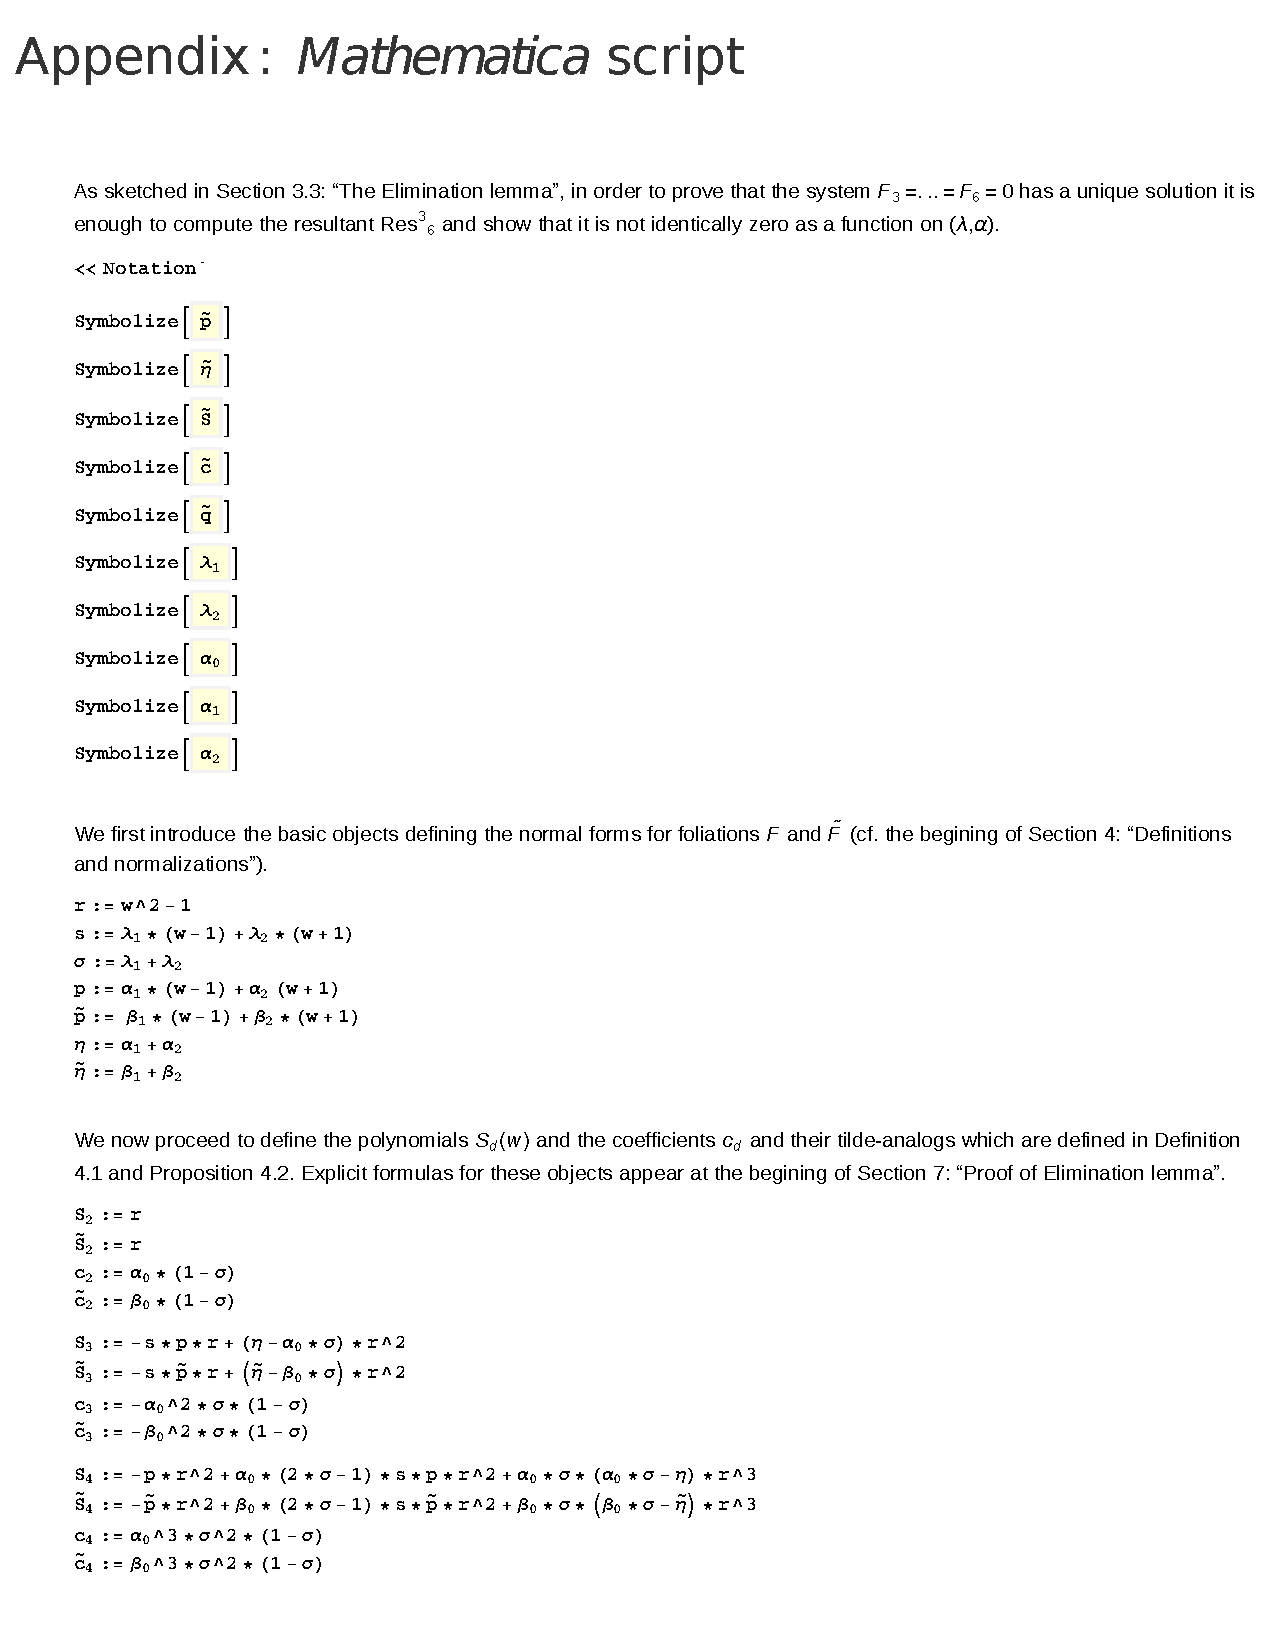
\includegraphics[scale=0.75]{Appendices/appendix1.pdf}\newpage
% 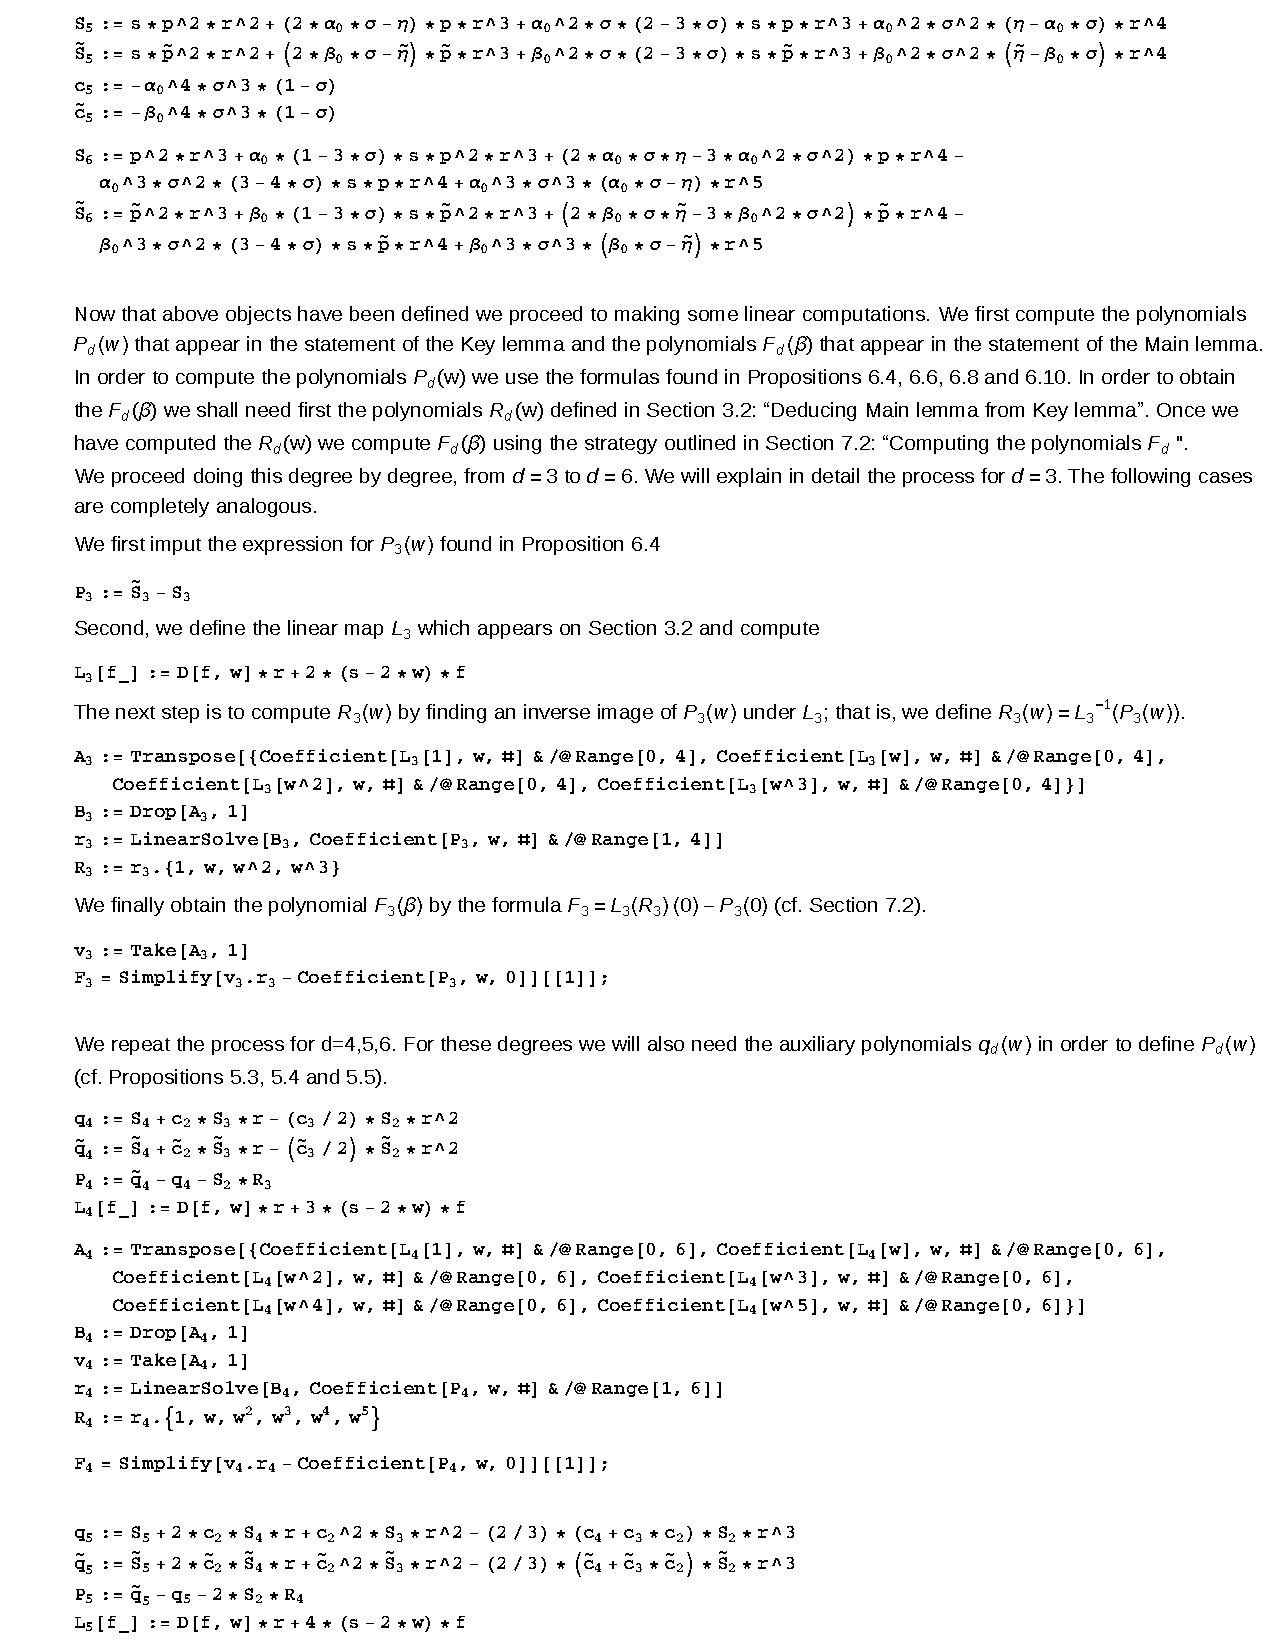
\includegraphics[scale=0.75]{Appendices/appendix2.pdf}\newpage
% 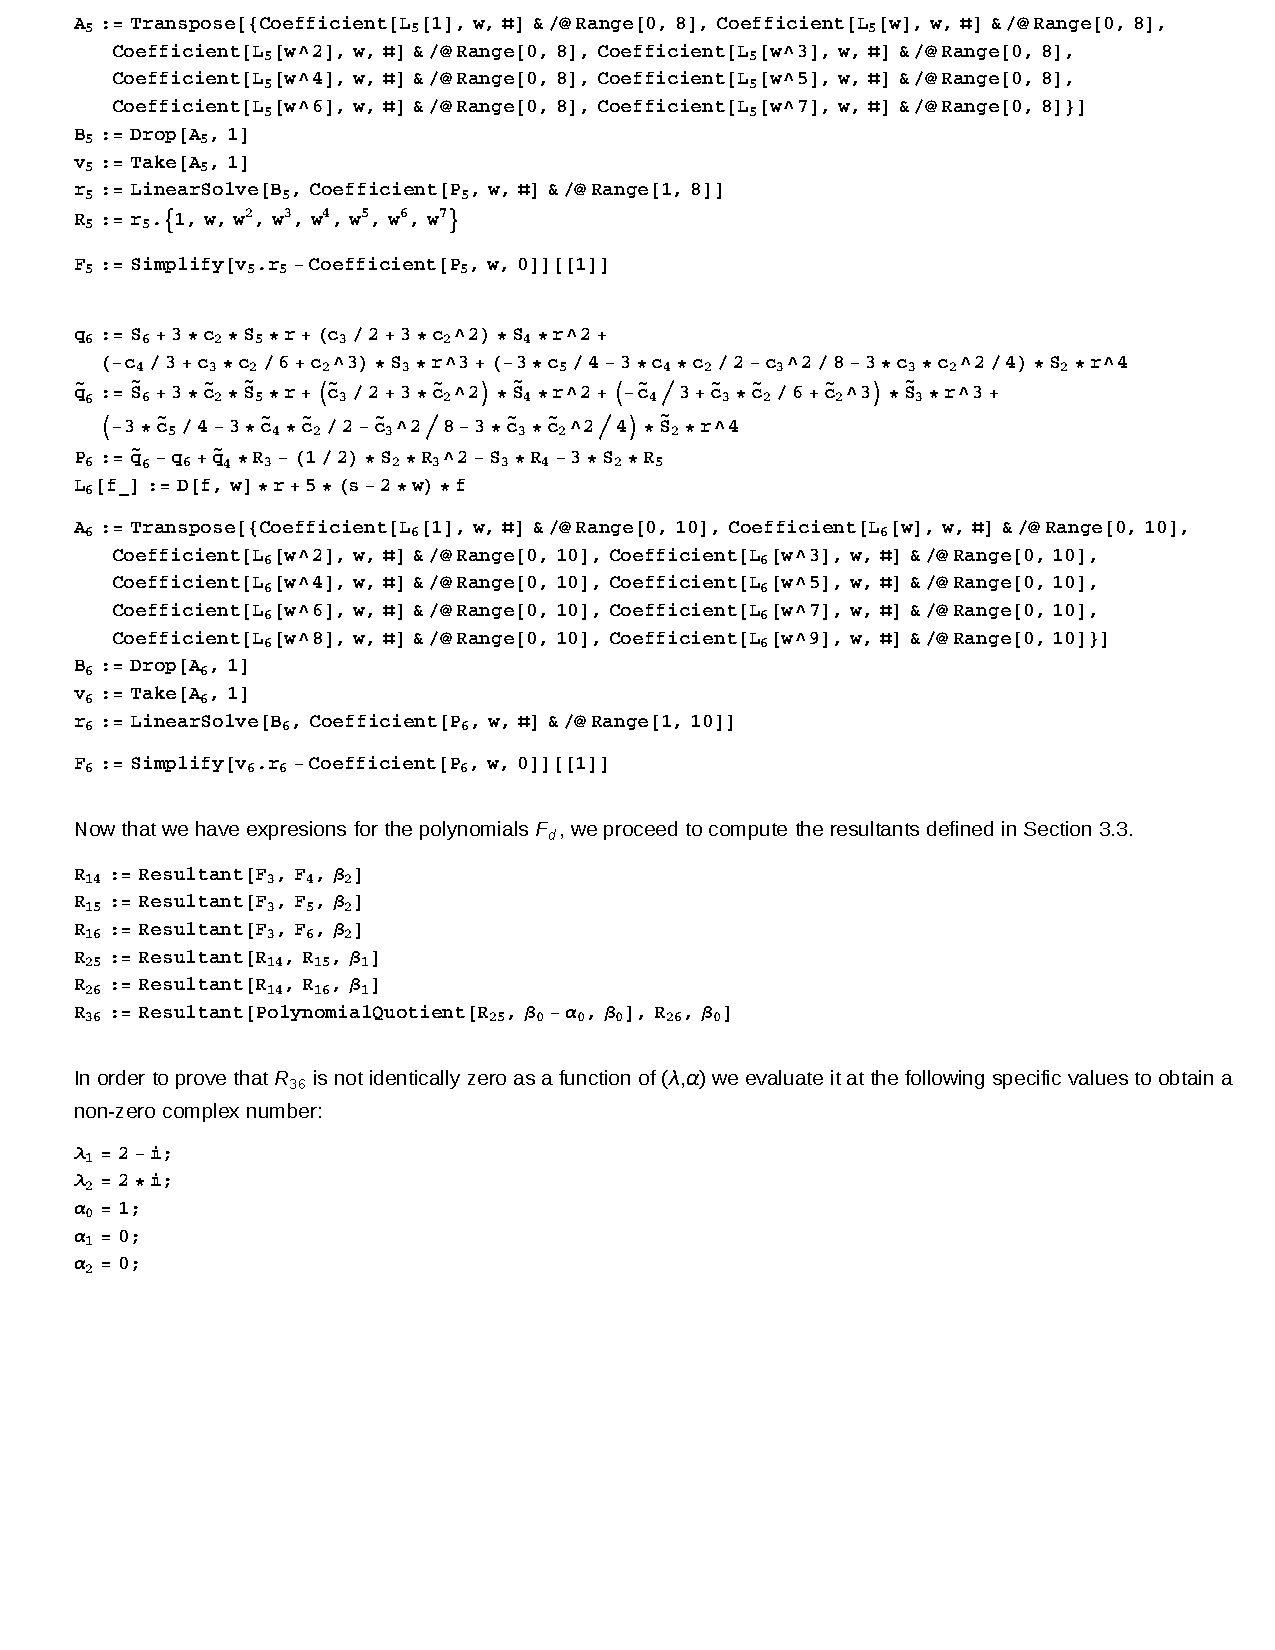
\includegraphics[scale=0.75]{Appendices/appendix3.pdf}\newpage
% 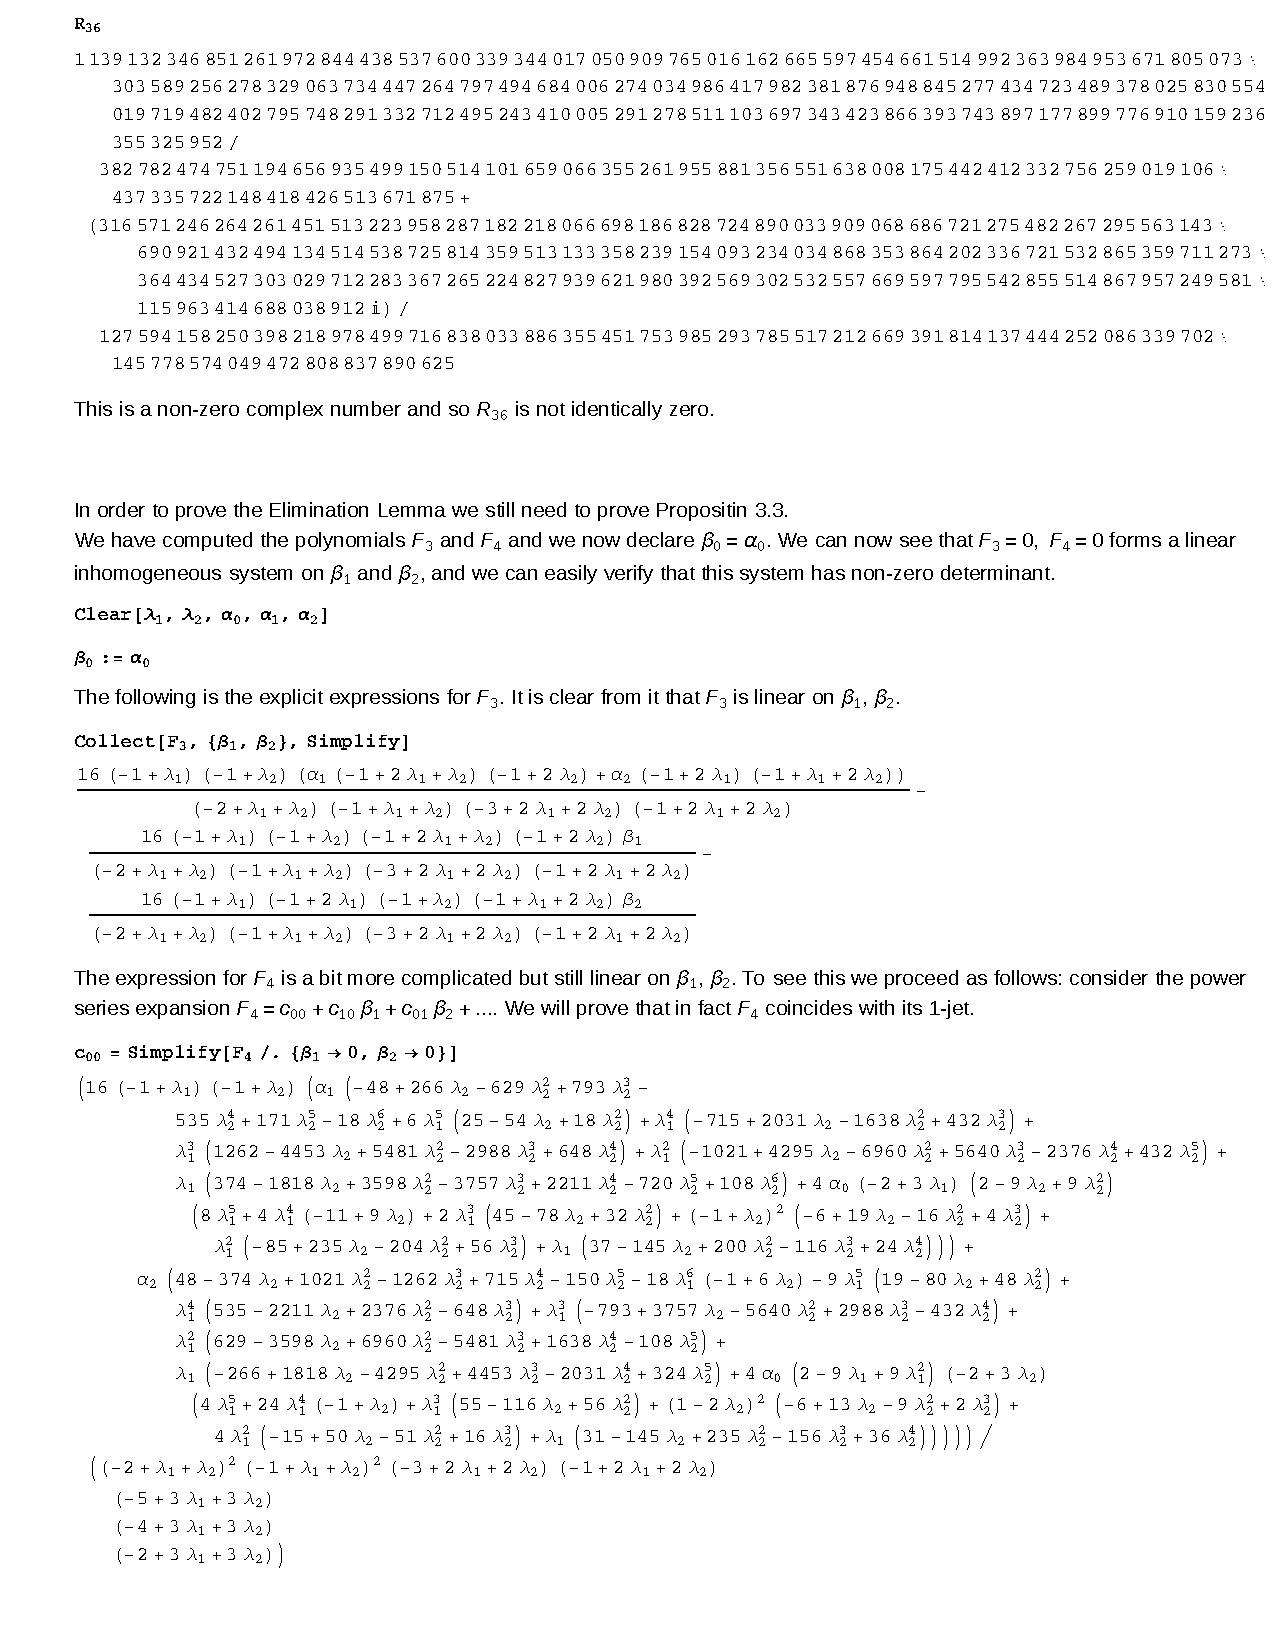
\includegraphics[scale=0.75]{Appendices/appendix4.pdf}\newpage
% 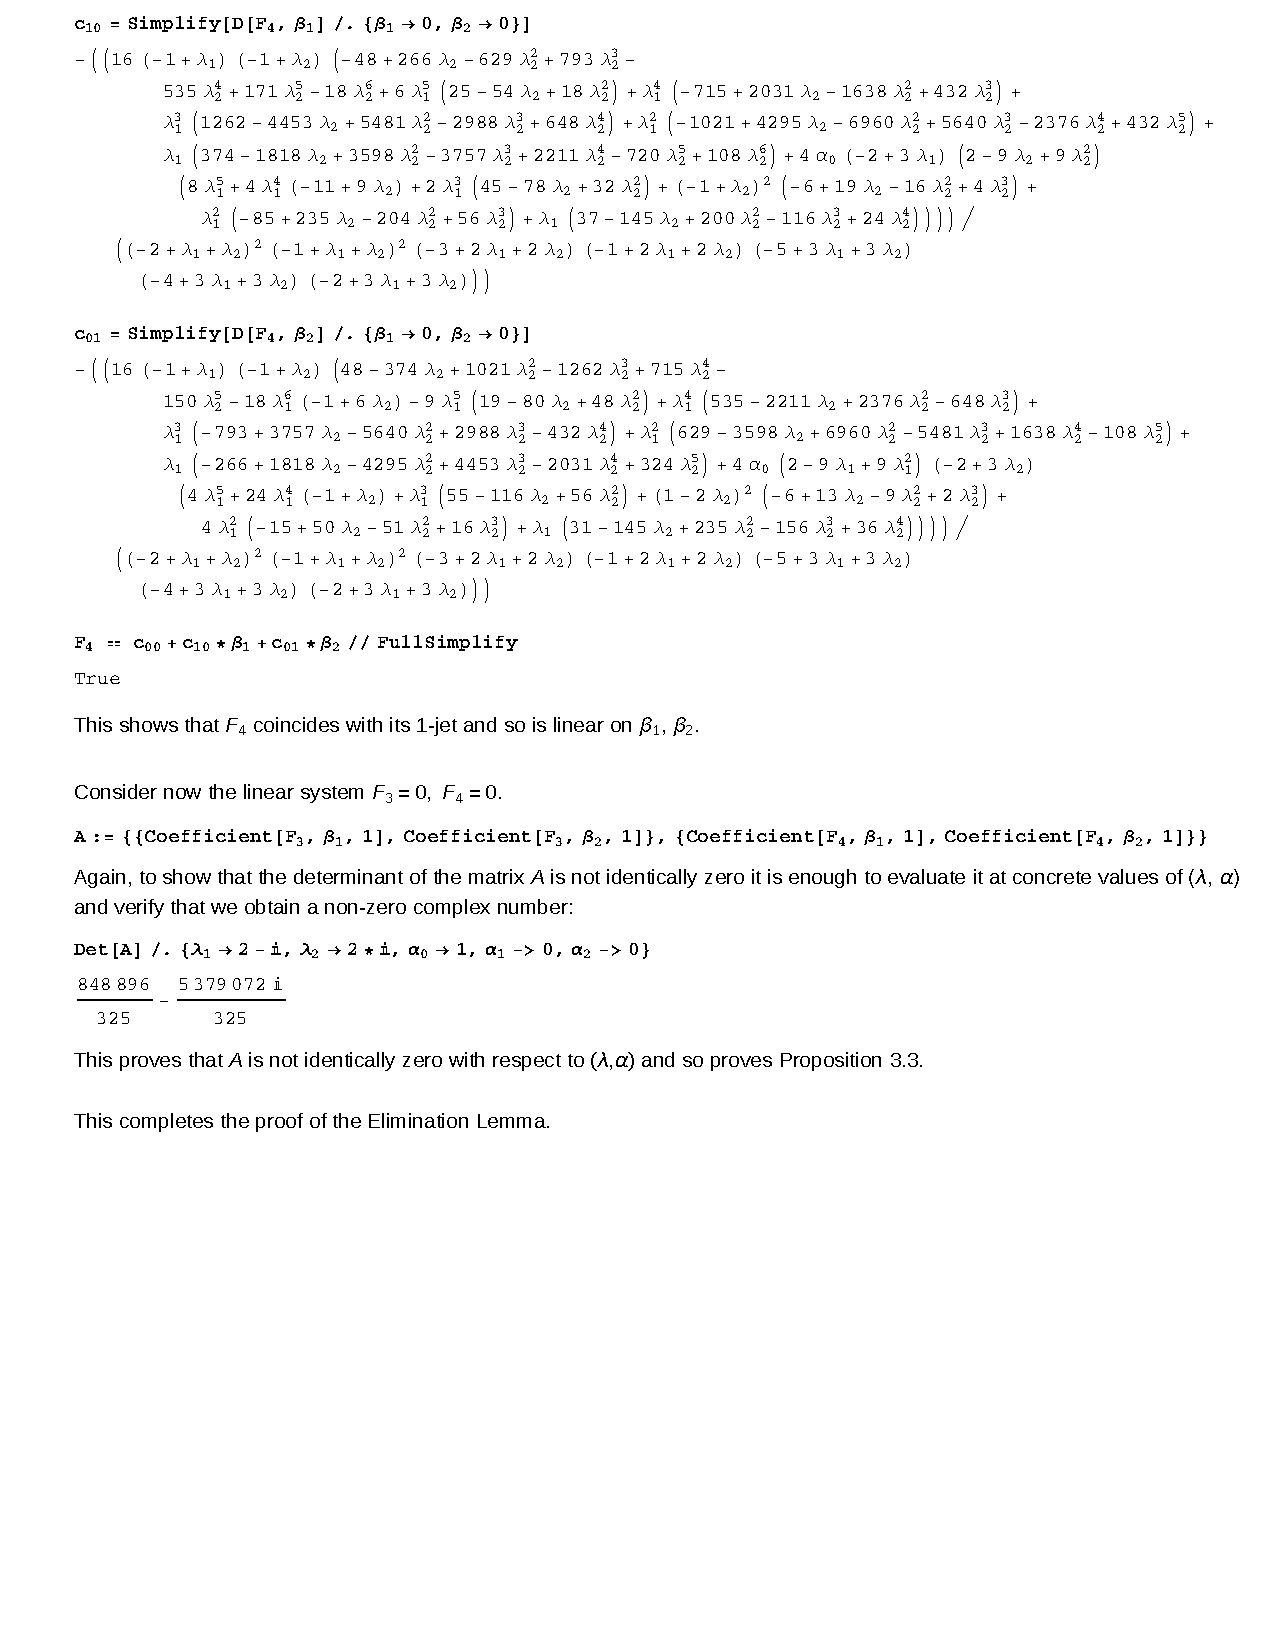
\includegraphics[scale=0.75]{Appendices/appendix5.pdf}\newpage
% \end{center}
% \end{changemargin}





\nocite{StrongTopoInvariance,UtmostRigidity,TwinVectorFields,WoodsHole,NoIndexTheorems}
\bibliography{ref-valente}

\end{document}




%%COMMENTS%%

% Restate theorems to make it easier to read?
% Review reference to appendices (label:%%APPENDIX%%) and citation of arXivVersion
% Thank Frank and cite Example in acknowledgements??
